\documentclass[12pt,a4paper,openright]{report} % use larger type; default would be 10pt
\usepackage{polski}
\usepackage[utf8]{inputenc} 
\usepackage{amsmath, amssymb,array,amsthm,enumerate,varioref,verbatim}
\usepackage[twoside,scale={0.75,0.8},marginratio={2:1,1:1}]{geometry}
\usepackage{graphicx} 
\usepackage{setspace}
\usepackage{array} 
\usepackage{paralist}
\usepackage{subfig} 
\usepackage{multirow}
\usepackage{epstopdf}
\usepackage{dcolumn}
\usepackage{bm}
\usepackage{fancyhdr} 
\usepackage{hyperref}
\usepackage[labelfont=bf]{caption}
\usepackage{fancyhdr}
\usepackage{dsfont}
\usepackage{tikz}
\usepackage{indentfirst}
\usepackage[nottoc,notlof,notlot]{tocbibind} 
\usepackage[titles,subfigure]{tocloft}
\usepackage[numbers,sort&compress]{natbib}
\usepackage{caption}
\captionsetup[figure]{labelsep=period}
\captionsetup{font={stretch=1.3}}
%
\pagestyle{fancy} \fancyhf{}
\fancyfoot[CE,CO]{\small\bfseries\scshape\thepage}
\fancyhead[CO]{\small\bfseries\scshape\rightmark}
\fancyhead[CE]{\small\bfseries\scshape\leftmark}
\usepackage{nomencl}
\makenomenclature
\renewcommand{\nomname}{Lista skrótów i oznaczeń}
\renewcommand{\labelitemi}{$\bullet$}
\linespread{1.4}
\renewcommand{\arraystretch}{1.5}
%
\begin{document}
%
%STRONA TYTULOWA------------------------------------------------------
%
\thispagestyle{empty}
\begin{center}
\large{POLITECHNIKA POZNAŃSKA \\
WYDZIAŁ FIZYKI TECHNICZNEJ}
\end{center}

\vspace{1cm}
\begin{center}
\large{\textbf{mgr inż. Szymon Maćkowiak}} \\
\end{center}

\vspace{2cm}

\begin{center}
\huge{\textbf{ROZPRAWA DOKTORSKA}}
\end{center}

\vspace{2cm}

\begin{center}
\large{\textbf{Własności tribologiczne układów cząsteczek w
geometrii szczeliny w warunkach kontrolowanego
ciśnienia badane metodą Dynamiki Molekularnej}}
\end{center}

\vspace{2cm}

\begin{center}
\textit{\large{Promotor \\ dr hab. Arkadiusz C. Brańka, prof. IFMPAN }}
\end{center}

\vspace{2cm}

\begin{center}
\large{Poznań 2016}
\end{center}
\newpage
%
%
%JEDNA PUSTA--------------------------------------------------------
\clearpage\thispagestyle{empty}
~
%STRESZCZENIE-------------------------------------------------------
%
\clearpage\thispagestyle{empty}
\noindent
\textbf{STRESZCZENIE}
\\

W rozprawie przedstawione zostały wyniki badań własności tribologicznych układów oddziałujących cząsteczek ograniczonych ruchomymi ścianami w warunkach zewnętrznego obciążenia oraz metoda Nierównowagowej Dynamiki Molekularnej.

W części metodologicznej omówiono problem symulowania układów w warunkach ograniczenia fizycznymi ścianami oraz wprowadzono nowy, mikroskopowy schemat kontroli temperatury, ciśnienia i ścinania w geometrii szczeliny. Zaproponowane równania ruchu zachowują pęd całkowity i pozwalają wprowadzić nowe wyrażenie na współczynnik tarcia, a ich postać oraz interpretacja znajduje uzasadnienie we współczesnych modelach tarcia.

W oparciu o zaproponowane równania ruchu, wykonano obliczenia dla układu typu szczeliny, zbudowanego z kilku tysięcy cząsteczek oddziałujących potencjałem Lennarda-Jonesa, ograniczonych ścianami krystalicznymi lub amorficznymi, w warunkach kontrolowanego ciśnienia, temperatury i ścinania.

Rozprawa omawia tworzące się stany stacjonarne i przedstawia otrzymane mapy stanów stacjonarnych, współczynnika tarcia i siły tarcia, zarówno dla układów ograniczonych ścianami krystalicznymi jak i amorficznymi.

Przeprowadzone badania pozwoliły zaobserwować i częściowo wyjaśnić szereg zjawisk takich jak nadśliskość, drgania cierne oraz negatywna wartość różniczkowego współczynnika tarcia. Pokazano istnienie związku pomiędzy tworzącymi się stanami stacjonarnymi a współczynnikiem tarcia w układzie oraz istotny wpływ chropowatości ograniczających ścian na właściwości tribologiczne układu.

\clearpage\thispagestyle{empty}
\noindent
\textbf{ABSTRACT}
\\ 

In this dissertation the research of tribological systems of interacting particles confined between moving walls under external load as well as the method of Non-equilibrium Molecular Dynamics have been presented. 

The problem of simulating systems confined between physical walls and the introduction of a new, microscopic scheme of temperature, pressure and shear rate control in the slit geometry have been presented in the methodological part. The proposed equations of~motion conserve total momentum of the system and allow to introduce a new expression for friction coefficient, while their form and interpretation is justified in modern models of friction. 

Based on the proposed equations of motion calculations for a slit model composed of several thousands of molecules interacting via Lennard-Jones potential, confined by crystalline and amorphous walls, under external pressure, temperature and shear rate control have been performed. 

The observed structures and obtained maps of stationary states, maps of friction coefficient and maps of friction force for both types of confinement between crystalline and amorphous walls have been presented. 

Performed simulations allowed to observe and partially explain such phenomena as superlubricity, stick-slip motion and negative differential coefficient of friction. The relation between the stationary states and the corresponding friction coefficient in the system have been noticed along with a significant impact of confining walls’ roughness on the tribological properties of the system.


%PODZIĘKOWIANIA
\clearpage\thispagestyle{empty}
\noindent
\vspace{15cm}
\begin{flushright}
\textit{Serdecznie dziękuję Panu Profesorowi IFMPAN Arkadiuszowi Brańce,\\
za naukową opiekę i wszelką pomoc w trakcie studiów doktoranckich \\
oraz wskazówki w czasie pisania tej pracy.\\
\vspace{1cm}
Dziękuję pracownikom Wydziału Fizyki Technicznej Politechniki Poznańskiej,
w~szczególności Profesorom Ryszardowi Czajce, Piotrowi Pierańskiemu, \\ Marianowi Radnemu 
oraz dr. hab. Arkadiuszowi Ptakowi, \\za pomoc i życzliwość na różnych etapach mojego doktoratu.\\
\vspace{1cm}
Dziękuję najbliższym, w których zawsze miałem wsparcie.}
\end{flushright}
%
%LISTA SYMBOLI-------------------------------------------------------
%
\clearpage\thispagestyle{empty}
\textbf{LISTA SYMBOLI I SKRÓTÓW}\\
\begin{spacing}{1.2}
\noindent
$\underline{F}$ $-$ siła\\
$\underline{p}$ $-$ pędy\\
$\underline{r}$ $-$ położenia\\
$U$ $-$ energia potencjalna układu\\
$K$ $-$ energia kinetyczna układu\\
$N$ $-$ liczba cząsteczek\\
$\mu$ $-$ współczynnik tarcia\\
$RWT$ $-$ różniczkowy współczynnik tarcia\\
$v_0$ $-$ zadana prędkość ścinania\\
$T_0$ $-$ zadana temperatura\\
$P_N$ $-$ zadane ciśnienie normalne\\
$LJ$ $-$ potencjał Lennarda-Jonesa\\
$WCA$ $-$ potencjał Weeks–Chandler–Andersen\\
$PH$ $-$ potencjał Petravic-Harrowell\\
$MD$ $-$ dynamika molekularna\\
$NEMD$ $-$ nierównowagowa dynamika molekularna\\
$NH$ $-$ termostat Nos\'{e}go-Hoovera\\
$VS$ $-$ skalowanie prędkości\\
$L$ $-$ stan ciekły\\
$CL$ $-$ stan centralnej lokalizacji\\
$SK\text{-}SL$ $-$ stan drgań ciernych\\
$PS$ $-$ stan nieruchomego czopu\\
$AM$ $-$ stan asymetrycznego topnienia\\
$MOP$ $-$ metoda płaszczyzn\\
$BG$ $-$ barostat globalny\\
$BM$ $-$ barostat mikroskopowy\\
$PT$ $-$ model Prandtla\\
$AFM$ $-$ mikroskop sił atomowych\\
$SFA$ $-$ aparat sił powierzchniowych\\
$QCM$ $-$ technika mikrowagi kwarcowej\\
$MEMS$ $-$ mikroukład elektroniczno-mechaniczny\\
$NEMS$ $-$ nanoukład elektroniczno-mechaniczny\\
$FF$ $-$ ograniczenie ścianami krystalicznymi\\
$RR$ $-$ ograniczenie ścianami amorficznymi\\
\end{spacing}
%
%SPIS TRESCI---------------------------------------------------------
%
\tableofcontents
%
%WSTEP---------------------------------------------------------------
%
\chapter{Wstęp}
%\addcontentsline{toc}{chapter}{Wprowadzenie}
\markright{Wprowadzenie}
%
Celem rozprawy doktorskiej jest opracowanie metody modelowania układów oddziałujących cząsteczek w geometrii szczeliny oraz zbadanie związku pomiędzy mikroskopowym tarciem a realizującymi się stanami stacjonarnymi, w warunkach kontrolowanego ciśnienia, ścinania i temperatury (warunki $T, v, P$).
Przedmiotem rozprawy są układy oddziałujących cząsteczek ograniczonych ruchomymi ścianami w warunkach zewnętrznego obciążenia oraz metody Nierównowagowej Dynamiki Molekularnej (\textit{ang.}~Non-equilibrium Molecular Dynamics - NEMD).

Cele rozprawy wiążą się ze zjawiskiem tarcia. Tarcie towarzyszy ludzkości od zarania dziejów. Jest obecne wszędzie tam, gdzie występuje wzajemny ruch powierzchni w bezpośrednim kontakcie lub rozdzielonych substancją smarującą. Najważniejszymi skutkami tarcia są straty energii i zużycie materiałów (np. ścieranie powierzchni). W zależności od okoliczności oczekuje się redukcji lub wzmożenia tarcia (np. redukcja wewnątrz układów mechanicznych lub zwiększenie między powierzchnią opon samochodowych i~nawierzchnią drogi) \cite{Hebda}. 
Mimo swojej powszechności, tarcie nadal pozostaje zjawiskiem nie~do~końca poznanym \cite{Persson2000, SpringerHandbook, Krim2002}. Makroskopowe aspekty tarcia zostały w dużej mierze opisane i usystematyzowane w drugiej połowie XX-tego wieku (w~ramach~nauki~technicznej - tribologii)~\cite{Hebda, Janecki}. W skali molekularnej wiele pytań, dotyczących istoty tarcia, nadal pozostaje otwartych. Wiąże się to ze złożonością procesów, których wynikiem \linebreak jest~tarcie~\cite{Dieriagin}.

Postępująca miniaturyzacja motywuje do poświęcenia szczególnej uwagi zjawiskom zachodzącym w skali mikroskopowej \cite{SpringerHandbook}. Wiele ograniczeń mikro- i nanotechnologii jest~następstwem~obecności~tarcia. Przykładem może być rozwój technik zapisu i odczytu danych w magnetycznych dyskach twardych. Obecnie względna prędkość współpracujących elementów (tzn. wirującego dysku i głowicy) dochodzi do 50 m/s. Dalsze zwiększenie szybkości zapisu i odczytu danych, wymaga rozwiązania problemu tarcia w skali mikroskopowej. W mikro- i nanoskali, wiele zjawisk fizycznych, w tym tarcie, zachowuje się inaczej niż w skali makroskopowej \cite{Szlufarska}. Przykładowo, w makroskali bardziej gładka powierzchnia wykazuje mniejszy współczynnik tarcia, natomiast redukcja chropowatości do rozmiarów mikro- i nanometrów powoduje drastyczne zwiększenie współczynnika tarcia \cite{Bowden, Bergli, Borys}. Wynika to ze wzrostu znaczenia adhezji powierzchni, która w przypadku makrochropowatości jest zaniedbywalna \cite{Bowden}. W nanoskali obserwuje się zmiany stanu skupienia płynu zawartego między dwiema współpracującymi powierzchniami \cite{Thompson, DMH1, Gattinoni2013}. Gdy grubość „smaru” jest ograniczona do kilkudziesięciu  pojedynczych warstw atomowych, stan smaru wykazuje wyraźną zależność od warunków zewnętrznych takich jak przyłożone obciążenie, czy prędkość przesuwania po sobie powierzchni (tzw.~prędkość ścinania). Stan smaru zaczyna również zależeć od liczby warstw molekularnych \cite{CuiCummings2001}. Wyniki badań eksperymentalnych i symulacji wskazują dodatkowo na możliwość tworzenia się nieobserwowanych w makroskali stanów stacjonarnych. Przykładowo, w skali molekularnej smar może ulec krystalizacji i przybrać formę nieruchomego czopu (tzw.~stan Plug-Slip) po którym ślizgają się powierzchnie ścian.

Podstawowe techniki eksperymentalne mikro- i nanotribologii to mikroskopia sił atomowych (Atomic Force Microscopy - AFM), technika mikrowagi kwarcowej \linebreak (Quartz Crystal Microbalance - QCM) oraz technika aparatu sił powierzchniowych \linebreak (Surface Force Apparatus - SFA) \cite{Krim2002, SpringerHandbook}. Obok metod eksperymentalnych duże znaczenie odgrywa modelowanie komputerowe, w szczególności symulacje Dynamiki Molekularnej~(MD)~\cite{SpringerHandbook, Martini2013, Vanossi2013}. 
%Metody obliczeniowe oparte na przybliżeniach ciągłych, nie uwzględniają efektów związanych z molekularną budową materii. 
%Z uwagi na powszechne uznanie Dynamiki Molekularnej, była ona podstawową techniką wykorzystaną w rozprawie.
Dynamika Molekularna była podstawową techniką obliczeniową wykorzystaną w rozprawie.
\begin{figure}[h!]
\centering
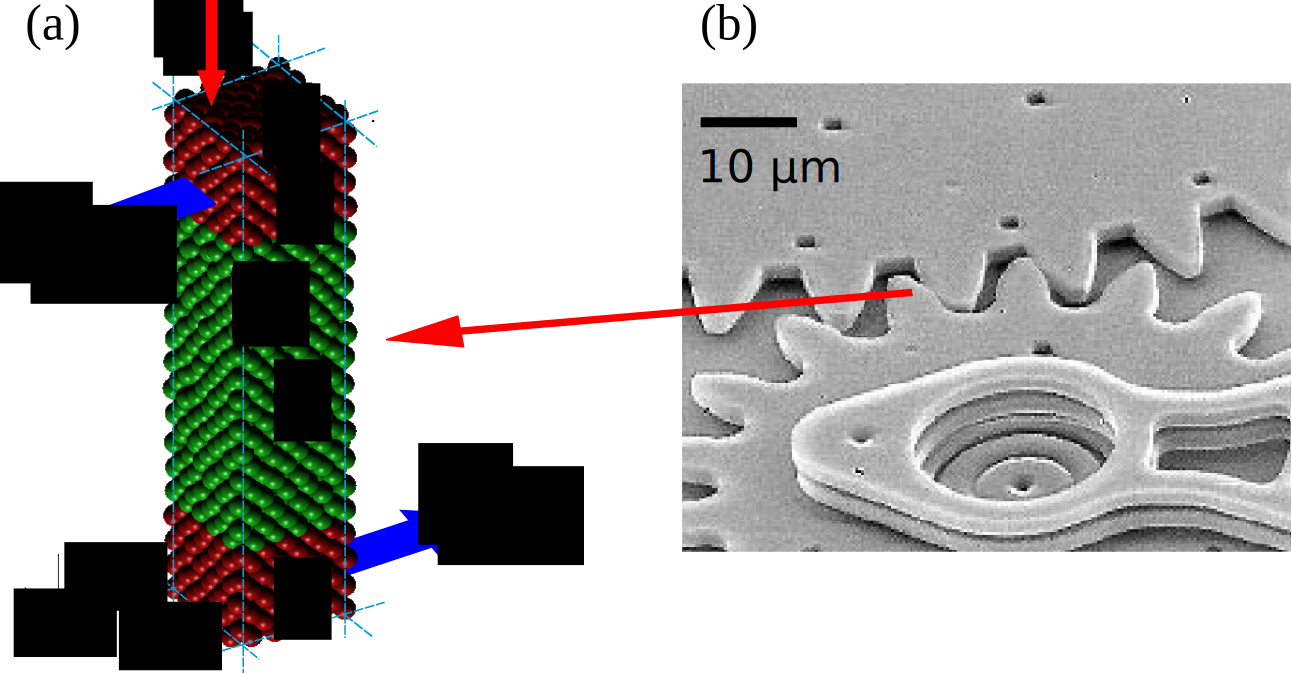
\includegraphics[width=14cm, clip]{rysunki/system_ABC}
\caption{Panel (a) - schemat geometrii układu. Obszary A i C reprezentują ograniczające ściany. Obszar B to układ ograniczonych cząsteczek. $P_N$ oznacza zadane ciśnienie, natomiast $v_0$ zadaną prędkość ścinania. Panel (b) - obraz układu kół zębatych, wykonany za pomocą Skaningowego Mikroskopu Elektronowego \cite{mems_photo}. Fragmenty interfejsu współpracujących powierzchni stanowią realizację geometrii szczeliny.}
\label{system_ABC}
\end{figure}
%Trudności metodologiczne
Ze względu na przestrzenne ograniczenie układu, symulacje MD można podzielić na symulacje układów objętościowych (\textit{ang.} bulk systems) oraz układów ograniczonych w zadanych kierunkach. Przedmiotem rozprawy są układy o~geometrii szczeliny, w której periodyczne warunki brzegowe stosuje się w kierunkach planarnych. Geometria szczeliny stanowi generyczny model tribologii.
Przykładowa realizacja geometrii mikroszczeliny została przedstawiona na rysunku~\ref{system_ABC}(a). Układ składa się z trzech części, które oznaczono kolejno symbolami A, B i C. Periodyczne warunki brzegowe zastosowano w kierunkach $x$ i $y$. W kierunku $z$ układ jest ograniczony ruchomymi ścianami A, C. Za pomocą ścian kontrolowane jest ciśnienie, ścinanie i temperatura układu.
Przykładem, realizującym model mikroszczeliny mogą być różne fragmenty współpracujących powierzchni wewnątrz mikroukładów elektroniczno-mechanicznych  (\textit{ang.} Micro Electro Mechanical Systems - MEMS). Przykład układu MEMS przedstawia rysunek~\ref{system_ABC}(b).
W~symulacjach układów ograniczonych zwykle zakłada się warunki stałej objętości, a~nie stałego ciśnienia \cite{hartkamp,LiemBrownClarke}. Wynika to głównie z nadal nierozwiązanych niedoskonałości metod symulacji układów mikroszczeliny w warunkach kontrolowanej temperatury $(T)$, ciśnienia $(P)$ i~prędkości ścinania $(v)$.

Modelowanie układu mikroszczeliny w warunkach $(T, v, P)$ stanowi jeden z głównych celów rozprawy, który wymaga rozważenia kilku istotnych zagadnień. 
%Schemat kolejności wykonanych prac, badań i testów dla części metodologicznej przedstawia rysunek \ref{metodologia}. 
%Ich rozwiązania zawierają się w czterech następujących obszarach.
Będą one przedmiotem rozdziału \ref{metody} i zostaną przeanalizowane w czterech następujących częściach.
\\
\\
\textbf{Budowa ścian.} W literaturze można znaleźć wiele sposobów ograniczania układu. Obecnie najpowszechniej stosowanym sposobem budowy ścian jest "wiązanie" atomów (za pomocą potencjału jednocząsteczkowego) do wirtualnych punktów przestrzeni, tworzących najczęściej sieć krystaliczną. Stosuje się zarówno potencjały harmoniczne \cite{Todd} jak i anharmoniczne \cite{ButlerHarrowell2003, PetravicHarrowell2006}. Problem wpływu typu stosowanego ograniczenia układu na jego właściwości jeste zwykle dyskutowany w niewielkim stopniu. W pracy pokazano, że modelowanie ścian za pomocą potencjałów jednocząsteczkowych może wpływać na~dynamikę i właściwości układu. Do najważniejszych konsekwencji należą niezachowanie całkowitego pędu w układzie, wytwarzanie niefizycznych drgań, które wpływają na~niektóre zjawiska tribologiczne (drgania cierne, sprzężenie tarcie-fonony), czy problemy z efektywnym odprowadzaniem ciepła przez ściany. W rozprawie zastosowano sposób budowy ścian bez zewnętrznych sprężyn, oparty na oddziaływaniu dwucząsteczkowym (sekcja \ref{conf}). 
\\
\\
\textbf{Kontrola temperatury.} Przyłożenie do układu ścinania wiąże się z wykonywaniem pracy nad układem i tym samym wzrostem temperatury. W celu uzyskania warunków stacjonarnych do układu należy dołączyć termostat, którego celem jest odprowadzanie ciepła, a w efekcie kontrola temperatury. Termostaty stosowane w symulacjach układów objętościowych były tematem wielu opracowań \cite{Nose1984, Hoover1985, Martyna1992, Branka2003, Branka2000, Braga2005, Andersen1980, Evans1983, Berendsen1984, Pieprzyk2015}. W układach ograniczonych \linebreak (typu szczeliny) kontrola temperatury nie była dotychczas przedmiotem tak intensywnych badań. Obecnie wiadomo, że termalizowanie układu w całej objętości, prowadzi do tworzenia się niefizycznych profili temperatury. Właściwym sposobem odbierania ciepła w warunkach ścinania jest kontrola temperatury przez ograniczające ściany \cite{DeLuca2014}. Nakładanie więzów (sprężyn) na układ powoduje problemy związane z bezpośrednim zastosowaniem termostatów. W rozprawie opracowano odpowiednie modyfikacje termostatu Nos\'{e}go-Hoovera \cite{Nose1984, Hoover1985} i skalowania prędkości \cite{Woodcock1971}, umożliwiające kontrolę temperatury w szczelinie (sekcja \ref{kontrola_temp}). 
\\
\\
\textbf{Obliczanie i kontrola ciśnienia.} W celu realizacji zadanej wartości makroskopowego ciśnienia, stosuje się tzw. barostaty. Warto podkreślić, że w odniesieniu do badania właściwości tribologicznych kontrola ciśnienia jest szczególnie ważnym zagadnieniem. Wiele makroskopowych praw tarcia dotyczy związku pomiędzy siłą tarcia a obciążeniem zewnętrznym. Podobnie jak w przypadku termostatów, schematy kontroli ciśnienia wykorzystywane w symulacjach układów ograniczonych różnią się od rozwiązań stosowanych w układach objętościowych \cite{andersen1980, ray82, Hoover86, ParrinelloRahman1980, ParrinelloRahman1981, QuigleyProbert2004, FallerdePablo02, UlineCortiI, EvansMorriss86, heyes1982}. W ramach rozprawy doktorskiej przetestowano stosowane dotychczas \cite{LupowskivanSwoll91a, LupowskivanSwoll91b, ButlerHarrowell2003, Pastewka2010} oraz zaproponowano nowe sposoby kontroli ciśnienia \cite{Gattinoni2014}. Schematy kontroli ciśnienia można podzielić na globalne i mikroskopowe. Działanie barostatów globalnych polega na dołączeniu do równań ruchu cząsteczek dodatkowego, "zewnętrznego" równania, które w zależności od obliczonej wartości chwilowego ciśnienia, zmienia względną odległość między ścianami ograniczającymi układ. Z zastosowaniem tych schematów wiąże się kilka trudności takich jak obliczanie chwilowego ciśnienia oraz konieczność doboru stałej sprzężenia zwrotnego. Ważnym wynikiem rozprawy jest zbudowanie schematu barostatu mikroskopowego, w którym człon odpowiedzialny za~kontrolę ciśnienia jest częścią równań ruchu cząsteczek \cite{Gattinoni2014}. Problem obliczania i kontroli ciśnienia został szczegółowo omówiony w sekcjach \ref{cisnienie} oraz \ref{barostaty}.\\
\\
\textbf{Kontrola ścinania.} Zjawisko tarcia wiąże się ze względnym ruchem powierzchni układu. Metody powszechnie wykorzystywane w literaturze polegają na bezpośrednim przemieszczaniu cząsteczek ścian o dystans odpowiadający zadanej prędkości ścinania \linebreak $ds=v_0dt$. Taki ruch może być również wywołany poprzez przyłożenie sił ścinających. W~rozprawie zastosowano metodę kontroli ścinania poprzez działanie odpowiednich sił na ograniczające ściany. Na podstawie wprowadzonych równań ruchu uzyskano nowe wyrażenie na współczynnik tarcia oparty na fluktuacjach względnej prędkości ścian. Schemat kontroli ścinania został szczegółowo omówiony i przetestowany w sekcji \ref{shearostat}.\\
%
%Opracowanie metody symulowania mikroszczeliny w warunkach kontrolowanego $(T, v, P)$ pozwoliło na przebadanie układu oddziałujących cząsteczek. 
%

Tribologiczne właściwości ograniczonych układów cząsteczek mają duże znaczenie praktyczne. Przykładem mogą być układy NEMS (\textit{ang.} Nano Electro Mechanical Systems) lub problem smarowania elastohydrodynamicznego (\textit{ang.} elastohydrodynamic lubrication - EHL), gdzie smar ograniczony jest ruchomymi powierzchniami w warunkach wysokiego ciśnienia i prędkości ścinania. Kontrola tarcia i smarowania w mikro- i nanoskali wymaga często innych rozwiązań niż w skali makroskopowej \cite{SpringerHandbook}. Przykładowo, zamiast płynnych polimerów rolę smaru mogą pełnić molekuły gazów szlachetnych. Zewnętrzne ciśnienie wpływa na powierzchnię rzeczywistego kontaktu współpracujących powierzchni oraz~na~własności reologiczne smaru. Symulacje NEMD oraz wyniki doświadczalne wskazują, że kiedy trące powierzchnie są rozdzielone cienką warstwą smaru, a prędkość ścinania jest relatywnie mała, chwilowy współczynnik tarcia może się zmieniać cyklicznie w czasie w formie tzw. "drgań ciernych" (\textit{ang.} stick-slip). W wyższych ciśnieniach, można spodziewać się krystalizacji smaru i utworzenia stanu, którego własności tribologiczne zależą od szczegółów jego struktury. 
%
\newpage
Bogactwo możliwych stanów stacjonarnych w układzie mikroszczeliny motywuje \linebreak do~ustalenia obszarów zadanej prędkości ścinania i normalnego ciśnienia $(v_0, P_N)$, które odpowiadają ich realizacji. Poszczególne stany stacjonarne charakteryzują się różnymi właściwościami fizycznymi. Z tego powodu kluczowym dla opisu własności tribologicznych układu jest określenie map tworzących się stanów stacjonarnych. Mapy stanów stacjonarnych oraz współczynnika tarcia pozwolą m. in. na wyznaczanie ścieżek optymalnego tarcia w procesach opartych na kontroli zewnętrznego ciśnienia i prędkości ścinania. Tworzące się stany stacjonarne mogą zależeć również od charakteru i chropowatości powierzchni ograniczających ścian. 

Pytania podejmowane w rozprawie dotyczą m. in. istnienie związku pomiędzy tworzącymi się stanami stacjonarnymi a współczynnikiem tarcia oraz wpływ rodzaju ograniczającej powierzchni na własności tribologiczne układu. Szczegółowy opis realizujących się stanów stacjonarnych oraz własności tribologicznych badanych układów przedstawiono w rozdziale \ref{wyniki}.
%
%
\chapter{Zjawisko tarcia}
%Aby wyjaśnić pewne założenia opracowanej metody, oraz zrozumieć część otrzymanych wyników, będę odnosić się do tzw. modeli/hipotez tarcia \cite{Borys, Janecki, Hebda, SpringerHandbook}. 
%
Zaproponowane metody i analiza wyników odnoszą się do modeli i hipotez tarcia. W~związku z~tym, najważniejsze z nich zostaną krótko omówione poniżej.

Tarcie jest złożeniem procesów opisywanych przez takie działy fizyki jak mechanika, termodynamika, fizyka statystyczna oraz mechanika płynów. Jest ono procesem nierównowagowym, a sama siła tarcia jest siłą niepotencjalną co czyni opis zjawiska dalece nietrywialnym. Dodatkowo redukcja rozmiarów współpracujących elementów może powodować ujawnienie efektów związanych z molekularną budową materii, których nie~uwzględnia opis makroskopowy \cite{DMH1}.
%
%
%

Wykorzystanie tarcia leży u zarania dziejów i łączy się z narodzinami cywilizacji \cite{Dieriagin}. Pierwsze rewolucje techniczne (opanowanie ognia, mielenie zbóż, wytwarzanie i ostrzenie narzędzi) wiązały się z wykorzystaniem przez człowieka tarcia. Źródła historyczne ukazują wczesne próby kontroli tarcia. Przykładami są m. in. utrwalone w egipskich hieroglifach polewanie drogi po której przesuwano kamienne bloki, podbijanie butów  rzymskich żołnierzy gwoźdźmi czy też wynalezienie i stosowanie w Chinach  pierwszych łożysk ślizgowych w młynach (celem usprawnienia procesu mielenia zboża) \cite{Hebda}.
%
%
%

Początek systematycznych badań zjawiska tarcia przypada na XV wiek. Pierwsze prawa tarcia sformułował wówczas Leonardo da~Vinci. Po nim problemem tarcia zajmowali się m. in. Amontons, Euler, Coulomb. W pierwszej połowie XX wieku duży wkład do wiedzy o tarciu wnieśli m. in. Bowden, Tabor, Dieriagin, Frenkel, Kontorova, Prandtl, Tomlinson i inni \cite{Borys}.
%
%
%

Wyodrębnienie nauki skoncentrowanej głównie na zjawisku tarcia nastąpiło w latach 60-tych XX wieku. W tym czasie rząd Wielkiej Brytanii zlecił opracowanie raportu na temat stanu brytyjskiej gospodarki grupie inżynierów pod kierownictwem \linebreak H. P. Josta \cite{Hebda}. Najważniejszy wniosek płynący z raportu dotyczył strat gospodarki brytyjskiej związanej z negatywnym wpływem zjawiska tarcia. Okazało się, że straty finansowe związane ze zużuciem części maszyn, stratami energii i materiałów sięgały ogromnej w tych czasach kwoty milionów funtów szterlingów. Uznano, że te znaczne straty finansowe były w dużej mierze konsekwencją niedostatecznego zrozumienia zjawiska tarcia oraz jego złej kontroli w procesach technologicznych. Aby zmienić ten stan rzeczy, zalecono m. in. wyodrębnienie interdyscyplinarnej nauki, której głównym przedmiotem będzie \linebreak zjawisko tarcia - tribologii. 

%
%
% 
Rodzaje tarcia można podzielić w oparciu o takie kryteria jak kryterium ruchu, lokalizacji, czy stanu skupienia obszaru pomiędzy współpracującymi powierzchniami. Schematycznie klasyfikację zjawiska tarcia ilustruje rysunek~\ref{klas_tar}.
\begin{figure}[h!]
\centering
\includegraphics[width=14cm, clip]{rysunki/klasyfikacja_tarcia.pdf}
\caption{Podział i klasyfikacja zjawiska tarcia na podstawie \cite{Janecki}.}
\label{klas_tar}
\end{figure}

Przed przyporządkowaniem problemu tarcia w układzie mikroszczeliny do konkretnej kategorii, zdefiniujmy poszczególne kryteria.
{Tarcie kinetyczne} (ruchowe) wiąże się ze~względnym przemieszczeniem dwóch ciał, przy czym jeżeli względna prędkość obszarów tarcia jest równa zeru, mówimy o tarciu {statycznym} (spoczynkowym). Ze względu na rodzaj ruchu tarcie kinetyczne jest dzielone na {tarcie ślizgowe}, w którym obszarem styku jest powierzchnia płaska lub zakrzywiona, oraz {tarcie toczne}, w którym obszarem styku elementów jest punkt (kontakt kul) lub linia (kontakt cylindrów). Szczególnym przypadkiem tarcia ślizgowego jest {tarcie wiertne}, w którym obszarem styku jest przekrój kołowy równocześnie przemieszczający się osiowo.   

W odniesieniu do układu omawianego w pracy oraz uwzględniając wprowadzoną klasyfikację można przyjąć, że szczególną uwagę poświęcono zjawisku tarcia kinetycznego ślizgowego $(1.2.1)$, o lokalizacji zewnętrznej między powierzchniami suchymi $(2.1.1)$ jak i wewnętrznej, zarówno w płynach i ciałach stałych $(2.2.1.1,~~ 2.2.1.2,~~ 2.2.2.1,~~ 2.2.2.2)$.
%
%
% 
\section{Historyczne hipotezy i modele tarcia suchego}
W pierwszej kolejności przedstawione zostaną hipotezy tarcia suchego \cite{Borys, Hebda, Janecki}, które niewątpliwie wpłynęły na rozwój współczesnej tribologii. Wskazane zostaną ich zalety oraz ograniczenia, które spowodowały konieczność rozwinięcia nowych modeli (w tym molekularnych). 
Mimo historycznego charakteru prezentowanych modeli, współcześnie (nawet w skali molekularnej), analizę wyników badań tarcia rozpoczyna się od konfrontacji z klasycznymi hipotezami. Z tego powodu w tej części pracy dokonano szerszego opisu modeli często nazywanych "historycznymi".  
%uwaga
%
\\
\\
\textbf{Hipoteza Leonarda da~Vinci (XV w.)} - pierwsze systematyczne badania zjawiska tarcia sięgają XV wieku i zostały wykonane przez Leonarda da~Vinci. Jego badania polegały na pomiarze siły jaką należy przyłożyć do ciała (a raczej ciężaru jaki należy przyłożyć do linki przerzuconej przez nieruchomy bloczek) aby wywołać ruch ciała na~powierzchni. Leonardo rozpatrywał zarówno przesuwanie po powierzchniach płaskich i~pochyłych. Kojarzonymi powierzchniami były kombinacje stali i drewna. Da~Vinci zauważył, że dwukrotne zwiększenie masy ciała spoczywającego na powierzchni, wymaga zastosowania dwukrotnie większej siły wymuszającej ruch. W ten sposób sformułował proporcjonalność siły tarcia od siły nacisku jakiej poddane było ciało. Zauważył niezależność siły tarcia od powierzchni kontaktu ciał (na podstawie badań tarcia liny zwiniętej w zwój i następnie rozciąganej). Sformułował następujące spostrzeżenie: "Zdolność ciał do ślizgania się jest różna i dlatego tarcie ma różną wartość" \cite{Borys}. To stwierdzenie odnosi się do gładkości - ciało o bardziej gładkiej powierzchni wykazuje mniejsze tarcie. Da~Vinci nie rozróżniał tarcia statycznego i kinetycznego.\\
\\
\textbf{Hipoteza Amontona (1699)} - niezależnie od Leonarda da~Vinci, zjawiskiem tarcia zajął się francuski uczony Guillaume Amontons (zapiski dotyczące dokonań Leonarda da~Vinci w dziedzinie rozumienia tarcia zostały odkryte później). Jego badania opierały się na pomiarach odkształcenia sprężyny w trakcie przesuwania przedmiotu (badania tarcia kinetycznego). Jego obserwacje były zasadniczo zbieżne z obserwacjami da~Vinciego. Jednak opis Amontona był pierwszym ilościowym ujęciem zjawiska tarcia. Obecnie dwa najczęściej stosowane prawa tarcia są nazywane prawami Amontona lub da~Vinciego-Amontona: I) wartość siły tarcia (kinetycznego) jest proporcjonalna do wartości siły normalnej, II) tarcie nie~zależy od powierzchni stykających się ciał.\\
Wprowadzając oznaczenia: $\mu$ - współczynnik tarcia, $F_f$ - siła tarcia, $F_N$ - siła nacisku, pierwsze prawo można zapisać w postaci wyrażenia $F_f=\mu F_N$. Współczynnik tarcia, $\mu = F_f/F_N$, mówi nam ile razy mniejszą siłę należy przyłożyć aby ciało przesuwać ze~stałą prędkością niż aby je podnosić ze stałą prędkością.\\
\\
\textbf{Hipoteza Belidora (1737)} - stanowi uzupełnienie modelu Amontona, w którym uwzględniono wspinanie się po sobie nierówności kulistych. W tym opisie powierzchnie ciał przybliżono układem twardych, jednakowych kul. Gdy układ jest w spoczynku, górna kula znajduje się między trzema kulami dolnej powierzchni. Aby wykonać przesunięcie górnej powierzchni na dolnej, każda górna kula musi się wspiąć na dwie z trzech kul podstawy. Wykonując stosowną analizę geometryczną, można pokazać, że uniwersalny współczynnik tarcia płynący z tej hipotezy przyjmuje wartość $\mu \approx 0.35$ \cite{Borys}.\\
\\
\textbf{Hipoteza Eulera (1748)} - Euler zaproponował kolejne uzupełnienie modelu Amontona, w którym założono wspinanie się jednej piłokształtnej powierzchni na drugą. W~odróżnieniu od modelu Belidora, założenie Eulera było bardziej obrazowe. W modelu Eulera, powierzchnię piłokształtną charakteryzuje kąt $\theta$. Współczynnik tarcia jest równy $\mu={F_f}/{F_N} = tg(\theta)$. Model Eulera stanowi, że siła tarcia zależy tylko od siły nacisku i~średniego kąta nachylenia nierówności. W ramach swoich rozważań Euler wyjaśnił również różnicę wartości tarcia statycznego i kinetycznego.\\
\\
\textbf{Hipoteza Coulomba (1781)} - ostatnim historycznym modelem tarcia suchego jest propozycja Coulomba oparta na modelu Eulera, ale wzbogacona założeniem elastycznego odginania nierówności i płynięcia po sprasowanych nierównościach. Rozważaniom Coulomba zawdzięczamy również sformułowanie III prawa tarcia - tarcie kinetyczne nie~zależy od prędkości ślizgania po sobie ciał. Zauważył również, że tarcie statyczne nie~jest stałe w czasie. Przykładowo, siła tarcia statycznego pomiędzy metalem pozostawionym na drewnianej powierzchni jest proporcjonalna do czasu \cite{Coulomb, Bartels}. Często jednak siła tarcia statycznego stabilizuje się w krótkim czasie, przez co efekt ten może być niezauważony. Model Coulomba pozwala wyrazić siłę tarcia jako $F_f = \mu F_N +A$, gdzie $A$ jest poprawką do wzoru Amontona i przedstawia część oddziaływania związaną z adhezją powierzchni trących. W modelu Coulomba $A$ jest stałą i nie zależy od nacisku ani od jakości powierzchni w kontakcie.\\

Przytoczone powyżej modele i płynące z nich hipotezy mają ograniczony zakres stosowalności. Najistotniejsze wady modeli historycznych wymieniono poniżej.
\begin{itemize}
\item{Brak mechanizmu rozpraszania energii. Problem można rozwiązać wprowadzając plastyczne odkształcanie nierówności (J. Leslie, 1804)\cite{Bowden1980}.}
\item{Sprzeczność z doświadczalnym efektem wzrostu tarcia ze stopniem wypolerowania metalowych powierzchni. Modele historyczne nie uwzględniają poprawnie zjawiska adhezji, która wzrasta w przypadku bardzo gładkich powierzchni i wywołuje sczepianie powierzchni.}
\item{Upatrywanie głównych przyczyn tarcia w chropowatości powierzchni co również nie znajduje potwierdzenia w doświadczeniu (W. Hardy, 1921-1928). Wykazano, że cienkie warstwy smaru dużo mniejsze od rozmiarów nierówności, znacznie redukują tarcie.}
\end{itemize}

Mimo swych ograniczeń, przedstawione modele tarcia suchego są często wykorzystywane w praktyce inżynierskiej, kiedy zgrubne oszacowania wartości tarcia są wystarczające. Modele historyczne można podsumować za pomocą trzech praw,
\begin{enumerate}[I.]
\item \textit{(da~Vinciego - Amontona) Wartość siły tarcia (kinetycznego) jest proporcjonalna do wartości siły normalnej.}
\item \textit{(da~Vinciego - Amontona) Tarcie nie zależy od powierzchni stykających się ciał.}
\item \textit{(Coulomba) Tarcie kinetyczne nie zależy od prędkości ślizgania po sobie ciał.}
\end{enumerate}
%
\section{Współczesne hipotezy tarcia suchego}
%
\label{modele_suche_wsp}
Modele historyczne wiążą przyczyny tarcia głównie z chropowatością przesuwanych po sobie powierzchni. Obecnie wiadomo jednak, że nierówności geometryczne nie są główną przyczyną oporów względnego ruchu. Już w 1734 roku John Theophilus Desaguliers zauważył, że dwie powierzchnie metalu można wypolerować tak mocno, że tarcie między nimi zaczyna wzrastać. Z kolei w latach 20-tych XX wieku, W. Hardy pokazał, że pokrycie powierzchni szkła warstwą tłuszczu o grubości dużo mniejszej niż wysokość chropowatości redukuje współczynnik tarcia z wartości 0.6 do 0.06. Przytoczone przykłady wskazują, że związek pomiędzy chropowatością a zjawiskiem tarcia nie jest prosty ani oczywisty. Ponieważ modele historyczne nie uwzględniają poprawnie wpływu zjawiska adhezji ani efektywnej powierzchni kontaktu współpracujących powierzchni, w~minionym stuleciu kontynuowano formułowanie hipotez tarcia.\\
\\
\textbf{Model Bowdena-Tabora (1939)} - jest hipotezą opartą na uogólnieniu obserwacji eksperymentalnych. Uwzględnia ona plastyczny charakter odkształceń na rzeczywistej powierzchni styku trących powierzchni ciał stałych. Sformułowana hipoteza mówi, że~wartość współczynnika tarcia i charakter uszkodzeń powierzchniowych powstałych w~czasie względnego ruchu powierzchni są określone głównie przez właściwości fizyczne powierzchni. Szczególnie istotne są: stosunek temperatur powierzchni, obciążenie, twardość materiału, temperatura topnienia. W oparciu o te założenia podzielono przypadki tarcia ślizgowego na trzy kategorie: 1) ślizganie metalu twardego po metalu miękkim, 2) metalu miękkiego po metalu twardym, 3) ślizganie metali o jednakowej twardości. 
Uznano, że~zjawisko tarcia powinno być traktowane tylko jako zjawisko powierzchniowe. W trakcie względnego przemieszczania powierzchni następuje tworzenie się i ścinanie metalicznych połączeń współpracujących części. Model uwzględnia, wpływ chropowatości na styk powierzchni w mikroobszarach oraz wpływ adhezyjnego sczepiania na efektywne tarcie. Zużycie powierzchni tłumaczy się jako efekt zespołu zjawisk związanych z adhezyjnym sczepianiem i tworzeniem metalicznych połączeń. Model Bowdena-Tabora pozwala wyznaczyć siłę tarcia jako sumę sił potrzebnych do ścięcia metalicznych połączeń ($F_s$) oraz plastycznego wyciśnięcia bruzd w bardziej miękkim metalu ($F_w$): $F_f = F_s + F_w$. Składowe siły tarcia można wyrazić jako $F_s = S \tau_{pt}$, oraz $F_w = S_w p_w$, gdzie $S$ to pole rzutu powierzchni styku, $\tau_{pt}$ - wytrzymałość na ścinanie połączeń metalicznych w kierunku stycznym do płaszczyzny tarcia, $S_w$ - przekrój poprzeczny bruzdy tarcia, $p_w$ - średni jednostkowy opór wywołany wyciskaniem metalu. Pole rzutu powierzchni styku można wyrazić jako $S={F_N}/\sigma_p$, gdzie $\sigma_p$ jest granicą plastyczności metalu o mniejszej twardości. Hipotezę Bowdena-Tabora można wyrazić równaniem na siłę tarcia $F_f = S \tau_{pt} + S_w p_w$, co w zakresie proporcjonalnej zależności $S$ od $F_N$ potwierdza I prawo tarcia (da~Vinciego - Amontona) \cite{Borys}. Model Bowdena i Tabora jest obecnie najważniejszym i powszechnie stosowanym modelem w zakresie konstrukcji maszyn.
%
\section{Molekularne hipotezy tarcia}
\label{mol_hip_tar}
Przedstawiony w sekcji \ref{modele_suche_wsp} model Bowdena-Tabora jest hipotezą mechaniczną i nie uwzględnia atomowej budowy materii. Postępująca miniaturyzacja wymaga uwzględnienia atomowego charakteru współpracujących powierzchni. Poniżej przedstawione zostaną najważniejsze modele i hipotezy tarcia uwzględniające atomową naturę materii. \\
\\
\textbf{Model Hertza (1882)} - 
przed omówieniem molekularnych hipotez tarcia, przedstawiona zostanie koncepcja jednostkowej chropowatości, szeroko stosowana w ramach eksperymentu AFM (mikroskop sił atomowych). Kiedy nierówność ulega sprężystemu odkształceniu (a nie plastycznemu płynięciu), kontakt można przybliżyć modelem dwóch stykających się powierzchni sferycznych o wypadkowym promieniu krzywizny $R$. \linebreak Hertz pokazał, że promień jednostkowego kontaktu między powierzchniami można wyrazić jako, $a=(3R F_N / 4E)^{1/3}$, gdzie $E$ jest modułem Younga. W przypadku odkształceń sprężystych, powierzchnia kontaktu skaluje się z obciążeniem, tzn. $S=\pi a^2 \sim F_N^{2/3}$. Dla~odróżnienia, teoria plastyczna zakłada, że $S \sim F_N$.\\
\\
\textbf{Model Greenwooda-Williamsona (1966)} - wynik Hertza wydaje się być sprzeczny z modelem adhezyjnym Bowdena-Tabora, w którym siła tarcia jest proporcjonalna do powierzchni kontaktu. W przypadku modelu Hertza należałoby przyjąć, że kontakt sprężysty nie spełnia praw da~Vinciego - Amontona i siła tarcia zamiast być proporcjonalna do $F_N$ jest proporcjonalna do $F_N^{2/3}$, co również nie znajduje potwierdzenia w~doświadczeniu. Trudność ta została rozwiązana przez Greenwooda i Williamsona, którzy założyli, że wypadkowy kontakt składa się z nierówności, które z kolei charakteryzują się pewnym rozkładem wysokości \cite{Borys, GreenWood}. Wzrost obciążenia $F_N$ powoduje nie tylko sprężyste odkształcenie wierzchołków. Wraz ze wzrostem odkształcenia rośnie liczba nierówności podpierających powierzchnie, w wyniku czego, przy odpowiednim rozkładzie nierówności, pole powierzchni wypadkowego kontaktu staje się proporcjonalne do obciążenia, $S \sim F_N$, \linebreak 
\\
co dalej prowadzi do wyników zgodnych z eksperymentem i prawami da~Vinciego - Amontona.
\\
\\
\textbf{Model Tomlinsona (1929)} - 
chociaż teorie mechaniczne w pewnym zakresie dość dobrze opisują zjawisko tarcia, nie tłumaczą jego przyczyn. Jednym z modeli, który odnosi się do tego problemu jest model Tomlinsona \cite{Janecki, Borys, Tomlinson1929}. Tomlinson przyjął, że tarcie jest konsekwencją oddziaływania atomów powierzchni. Ponieważ powierzchnie są chropowate, poszczególne punkty materialne tych powierzchni są różnie oddalone względem siebie. Dodatkowo odległość między nimi jest zmienna w czasie. Z tego powodu tylko niektóre punkty będą w bezpośrednim kontakcie. W związku z tym pewne punkty powierzchni będą się przyciągać a inne odpychać. W pewnych przypadkach siły przyciągające mogą zdominować siły odpychające i wówczas dochodzi do "sklejenia" powierzchni. W założeniu Tomlinsona suma sił przyciągających jest mała i można ją pominąć. Z kolei obciążenie normalne jest równoważone siłami odpychania. W trakcie względnego przesuwania powierzchni jedne cząsteczki odrywają się od drugich, wychodzą z jednych obszarów oddziaływań i przechodzą do kolejnych. Ciągła zmiana par oddziałujących cząsteczek, zrywanie oraz tworzenie nowych połączeń wiąże się z rozpraszaniem energii. Tomlinson pokazał, że związek pomiędzy mikroskopowym współczynnikiem tarcia a stratami energii $E$, ma postać $\mu = E/(l p)$, gdzie $l$ to średnia odległość między cząsteczkami a $p$ to średnia siła potrzebna do rozerwania pojedynczej pary cząsteczek. Model Tomlinsona wiąże przyczyny tarcia głównie z międzyatomową adhezją oraz nie uwzględnia innych mechanizmów rozpraszania energii kinetycznej w układzie.
\\
\\
\textbf{Model Prandtla (1928)} - w tym modelu cząsteczka lub układ cząsteczek jest przyczepiony za pomocą sprężyn do ruchomych punktów przesuwających się nad powierzchnią zdefiniowaną za pomocą periodycznego potencjału \cite{Prandtl1928}. Mimo swej prostoty model Prandtla (PT) pozwala wyciągnąć wiele istotnych wniosków \cite{SpringerHandbook, Popov2014}. W najprostszym przypadku, model Prandtla można przedstawić w formie cząsteczki wiedzionej przez sprężynę, nad powierzchnią periodycznego potencjału, tak jak przedstawia to rysunek \ref{PTmodel}. 
\begin{figure}[h!]
\centering
\includegraphics[width=10cm, clip]{rysunki/PTmodel.pdf}
\caption{Ilustracja modelu Prandtla. Powierzchnię reprezentuje periodyczny potencjał. $F_0$ oznacza maksymalną siłę jaką powierzchnia działa na cząsteczki. Stałe sieciowe układu cząsteczek i powierzchni to odpowiednio $a$ i $b$. Pozycja i prędkość wybranej cząsteczki to $x$ i $\dot{x}$. Cząsteczki są przyczepione za pomocą sprężyn do ruchomych punktów. Pozycja i prędkość wybranego punktu to $x_0$ i $v_0$. Rysunek na podstawie \cite{SpringerHandbook}.}
\label{PTmodel}
\end{figure}
Punkt zaczepienia sprężyny przemieszcza się ze stałą prędkością. Równanie ruchu cząsteczki ma postać:
\begin{equation}
m\ddot{x}=-F_0 sin(x) + k(v_0 t - x)-\eta \dot{x},
\end{equation}
gdzie $\eta$ jest stałą tłumienia. Przy dostatecznie małej wartości $k$, wyraz $k(v_0 t -x)$ może być traktowany jako stały. W takim przypadku model Prandtla przyjmuje postać
\begin{equation}
m\ddot{x}=-F_0 sin(x) + F -\eta \dot{x},
\end{equation}
gdzie $F$ ma stałą wartość. Jest to granica "miękkiej sprężyny" modelu Prandtla. Model Prandlta w granicy miękkiej sprężyny pozwala rozróżnić tarcie statyczne i kinetyczne. Tarcie kinetyczne zachodzi wówczas, gdy $\eta \dot{x} \geqslant F_0$. Po przekroczeniu wartości tarcia statycznego, cząsteczka rozpoczyna ciągły ruch pod wpływem przyłożenia siły o mniejszej wartości niż graniczna wartość $F_0$. Jest to też proste wyjaśnienie, dlaczego współczynnik tarcia kinetycznego ma mniejszą wartość od współczynnika tarcia statycznego \cite{Popov2014}. Model Prandtla w granicy "miękkiej sprężyny" będzie wykorzystany w pracy w sekcji \ref{shearostat}.
\\
\\
\textbf{Model Frenkela-Kontorova (1938)} - w wielu aspektach jest podobny do modelu Prandtla, jednak cząsteczki nie są związane z ruchomymi punktami, ale są połączone ze~sobą wzajemnie  \cite{SpringerHandbook, Frenkel1938}. Ideę modelu Frenkela-Kontorova (FK) przedstawia rysunek \ref{FKmodel}. 
\begin{figure}[h!]
\centering
\includegraphics[width=10cm, clip]{rysunki/FKmodel.pdf}
\caption{Ilustracja modelu Frenkela-Kontorova. Powierzchnię reprezentuje periodyczny potencjał. $F_0$ oznacza maksymalną siłę jaką powierzchnia działa na cząsteczki. Stałe sieciowe układu cząsteczek i powierzchni to odpowiednio $a$ i $b$. Pozycja i prędkość wybranej cząsteczki to $x$ i $\dot{x}$. Cząsteczki są połączone ze sobą za pomocą sprężyn. Rysunek na podstawie \cite{SpringerHandbook}.}
\label{FKmodel}
\end{figure}
Model ten przede wszystkim ujawnia i wyjaśnia dwa zjawiska. Pierwszym jest udział fononów w rozpraszaniu energii kinetycznej przesuwanych po sobie powierzchni. Oddziaływanie pomiędzy wzajemnie przesuwanymi "łańcuchami" atomów powoduje, że~ich energia ruchu postępowego zamienia się w czasie w energię ruchu drgań wewnętrznych (między atomami). Drugim interesującym zjawiskiem jest nadśliskość, które może pojawić się gdy stałe sieciowe przesuwanych powierzchni są różne, a ich stosunek nie jest liczbą wymierną. Układ powierzchni, dla których stosunek stałych sieciowych nie jest liczbą wymierną nazywa się niewspółmiernymi \cite{SpringerHandbook}. Pojęcie niewspółmierności pozwala rozróżnić przesuwanie po sobie takich samych lub różnych powierzchni. W modelu Frenkela-Kontorova wzajemne przesuwanie niewspółmiernych powierzchni (po pokonaniu oporów statycznych) wiąże się z gromadzeniem energii w odkształceniach sprężyn łączących cząsteczki. Po pokonaniu studni potencjału powierzchni, energia ta zostaje uwolniona i rozpoczyna się ruch z wyjątkowo niską wartością współczynnika tarcia. Podobny efekt został obserwowany w układach rzeczywistych \cite{SpringerHandbook, Krim2002} oraz w przeprowadzonych symulacjach (rozdział \ref{wyniki}).   
%
\section{Hipotezy tarcia wewnętrznego w płynach}
\noindent
\textbf{Model Dieriagina (1952)} - w przypadkach rozważanych w tej rozprawie nie będziemy mieć do czynienia z czystym tarciem suchym, a raczej z mieszaniną tarcia suchego i tarcia wewnętrznego. Z tego powodu warto krótko wspomnieć modele dotyczące molekularnego pochodzenia tarcia w płynach. Dieriagin \cite{Dieriagin} wyjaśnia opory ruchu w układzie powierzchni rozdzielonych płynem dwoma efektami. Pierwszy dotyczy zderzeń płynu z chropowatą powierzchnią. Zderzenia z molekułami płynu, których charakter jest przypadkowy, powodują rozpraszanie energii kinetycznej ruchu postępowego ścian i zamieniają się w energię ruchu chaotycznego. Drugi efekt mający wpływ na tarcie to niesprężyste zderzenia cząsteczek ze ścianami oraz ich adsorpcja. Powyższą koncepcję przedstawia rysunek \ref{DGmodel}. Panel (a) przedstawia zderzenie idealnie sprężyste cząsteczki z gładką ścianą. Cząsteczka odbita od idealnie gładkiej i sprężystej powierzchni nie wymienia ze ścianą składowej pędu w kierunku poślizgu. Panel (b) przedstawia sytuację, w której cząsteczka padając na chropowatą powierzchnię przekazuje jej część swojego pędu na skutek zderzenia. Dodatkowo straty pędu w układzie wiążą się ze zderzeniami niesprężystymi oraz adsorpcją cząsteczek na powierzchni ograniczającej ściany.
\begin{figure}[h!]
\centering
\includegraphics[width=8cm, clip]{rysunki/DGmodel.pdf}
\caption{Ilustracja modelu Dieriagina. Panel (a) przedstawia sytuację idealnie sprężystego zderzenia cząsteczki płynu z gładką ścianą. W takim przypadku kolizja cząsteczki o prędkości $v$ i ściany o prędkości $u$ nie wpływa na straty energii kinetycznej uporządkowanego ruchu w układzie. Panel (b) przedstawia kolizję niesprężystą z powierzchnią chropowatą. W tej sytuacji zderzenie wywołuje straty energii kinetycznej uporządkowanego ruchu cząsteczek co stanowi wkład do makroskopowego tarcia. Dodatkowo cząsteczki mogą ulec adhezji. Rysunek na podstawie \cite{Dieriagin}.}
\label{DGmodel}
\end{figure}
Oba efekty mają wpływ na statystykę zderzeń cząsteczek płynu z ograniczającymi ścianami oraz zamianę energii kinetycznej uporządkowanego ruchu na ruch chaotyczny. Można spodziewać się, że modyfikacja powierzchni, wpływa na charakter zderzeń i wymianę pędu pomiędzy cząsteczkami płynu a powierzchni oraz zmienia tarcie w układzie. 
\\
\\
\textbf{Model Petravic (2008)} - w ostatnich latach interesujące wyjaśnienie natury zjawiska tarcia wniosły prace J. Petravic i P. Harrowella \cite{Petravic2, PetravicHarrowell2006, Petravic2006-2, Petravic2005}. Prace dotyczą m. in. właściwości współczynników transportu (w tym współczynnika tarcia) w ramach teorii odpowiedzi liniowej \cite{EvansMoris1990}. W pracy \cite{Petravic2} rozważany jest problemem zaniku współczynnika tarcia cząsteczki poruszającej się w płynie. Jeżeli masa cząsteczki i płynu jest skończona, współczynnik tarcia w układzie zanika z czasem do zera, ponieważ uporządkowany ruch (pęd) ulega rozproszeniu. Podobnie, jeśli cząsteczka będzie mieć nieskończoną masę, doprowadzi do sytuacji, w której płyn będzie mieć taką samą prędkość jak cząsteczka i współczynnik tarcia ulegnie zanikowi. Zgodnie z wnioskami Petravic, aby uzyskać~w układzie nieznikający w czasie współczynnik tarcia, konieczna jest obecność co najmniej dwóch nieskończenie dużych mas we względnym ruchu. Powyższe wnioski wykorzystano w metodzie zaproponowanej w rozprawie w rozdziale \ref{metody}.
%
\chapter{Metoda symulacji tarcia w mikroszczelinie}
\label{metody}
W tym rozdziale przedstawiony zostanie opracowany schemat NEMD dla układów ograniczonych w geometrii szczeliny, w warunkach kontrolowanego $(T, v, P)$ (gdzie $T$ - temperatura, $P$ - ciśnienie normalne, $v$ - prędkość ścinania). Geometrię szczeliny przedstawia rysunek \ref{szczelina}. 
\begin{figure}[h!]
\centering
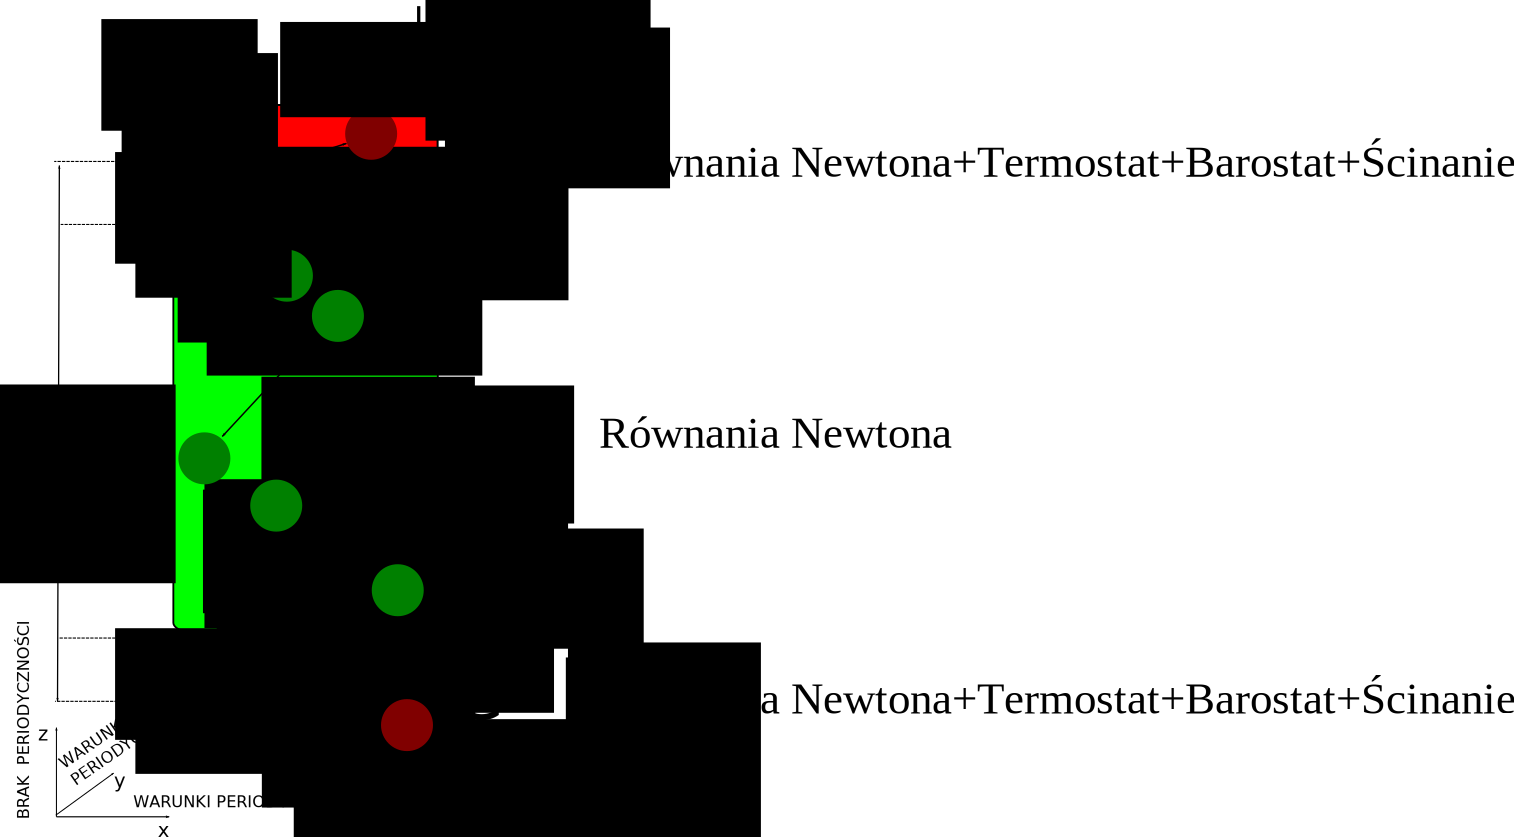
\includegraphics[width=15cm, clip]{rysunki/szczelina.pdf}
\caption{Ilustracja geometrii szczeliny. Obszar B to układ cząsteczek ograniczonych ścianami. Obszar A i C to ściany układu, za pomocą których prowadzona była również kontrola temperatury, ciśnienia i ścinania. Oddziaływania dwucząsteczkowe w poszczególnych obszarach (oraz pomiędzy obszarami) oznaczono jako $u_{AA}, u_{AB}, u_{BB}, u_{BC}, u_{CC}$, gdzie indeksy A, B, C, oznaczają lokalizację oddziałujących cząsteczek. Periodyczne warunki brzegowe są zastosowane w kierunkach $x$ i $y$. $P_N$, $v_0$, $T_0$ to odpowiednio zadana wartość ciśnienia zewnętrznego, prędkość ścinania i temperatura ścian. $S$ i $L$ oznaczają odpowiednio pole przekroju poprzecznego układu w płaszczyźnie $xy$ oraz szerokość układu zdefiniowaną jako dystans pomiędzy środkami mas ograniczających ścian.}
\label{szczelina}
\end{figure}
Układ składa się z trzech części. Obszary A i C (na rysunku \ref{szczelina} zaznaczone kolorem czerwonym) to ściany układu. Obszar B (zaznaczony kolorem zielonym) to układ ograniczonych cząsteczek. Ruch cząsteczek w obszarze B opisują równania Newtona. Z kolei równania ruchu cząsteczek w obszarach A i C są rozszerzone o wyrażenia odpowiedzialne za kontrolę temperatury, ciśnienia i ścinania. Periodyczne warunki brzegowe są zastosowane w kierunkach $x, y$. W kierunku $z$ układ jest ograniczony fizycznymi ścianami. Opracowanie schematu, pozwalającego na równoczesną kontrolę temperatury, ciśnienia i ścinania w takim układzie, wymagało rozwiązania określonych zagadnień. Kolejność dyskutowanych problemów oraz plan tego rozdziału ilustruje rysunek \ref{metodologia}. 
\begin{figure}[h!]
\centering
\includegraphics[width=14cm, clip]{rysunki/metodologia_v2.pdf}
\caption{Schemat tworzenia metody NEMD dla układu szczeliny w warunkach kontrolowanego $(T, v, P)$. Kolejne dyskutowane zagadnienia to: 1) budowa ścian, 2) kontrola temperatury, 3) kontrola ciśnienia, 4) kontrola ścinania. Rozwiązania problemów 1-4 składają się na schemat końcowy, wykorzystany do zbadania właściwości tribologicznych układu mikroszczeliny.}
\label{metodologia}
\end{figure}
%
W pierwszej części zostanie omówiony sposób budowania ścian ograniczających układ. Następnie omówione zostaną kolejno opracowane schematy kontroli temperatury, ciśnienia i ścinania.
\section{Budowa ścian}
\label{conf}
Podstawową różnicą pomiędzy geometrią szczeliny a geometrią układów objętościowych jest ograniczenie układu fizycznymi ścianami w wybranym kierunku. Zmiana warunków brzegowych może istotnie wpływać na właściwości fizyczne układu. \\Rozwój podejścia do problemu przestrzennego ograniczania układu przedstawia \linebreak rysunek~\ref{ewolO}.
%
\begin{figure}[h!]
\centering
\includegraphics[width=12cm, clip]{rysunki/ewolucjaOGR.pdf}
\caption{Ilustracja stosowanych sposobów ograniczania układu w geometrii szczeliny.}
\label{ewolO}
\end{figure}
%
Najprostszym i najwcześniej stosowanym rozwiązaniem jest ograniczenie układu za pomocą gładkich, monolitycznych ścian. Praktyczna realizacja opiera się na~zastosowaniu odpowiedniego potencjału odpychającego. Innym, bardziej zbliżonym do~rzeczywistej sytuacji rozwiązaniem było zastosowanie ścian strukturalizowanych. Jednak sztywne powierzchnie atomowe nie oddają rzeczywistego charakteru zderzeń cząsteczek ograniczonej części ze ścianami \cite{Bernardi2010}. Obecnie często stosowanym rozwiązaniem, jest wiązanie cząsteczek tworzących ściany do punktów wirtualnej sieci krystalicznej. Polega ono na uwzględnieniu w dynamice ruchu cząsteczek, dodatkowej, jednocząsteczkowej siły zależnej od odległości pomiędzy położeniem cząsteczki a węzłem sieci. W literaturze stosuje się zarówno siły harmoniczne i anharmoniczne \cite{Todd, PetravicHarrowell2006, DMH1}. W tej części rozprawy omówione zostaną wybrane aspekty tworzenia ścian układu za pomocą oddziaływania z~węzłami sieci krystalicznej. \\
%
%
%
Zastosowanie warstw atomowych, unieruchomionych w przestrzeni lub przyłączonych do~węzłów sieci, wpływa na cząsteczki jak zewnętrzna, jednocząsteczkowa siła. Jej działanie powoduje niezachowanie całkowitego pędu, momentu pędu i środka masy układu. W~konsekwencji układ odniesienia staje się nieinercjalny, a w układzie działają pozorne siły bezwładności. Dodatkowo, monitorowanie całek ruchu takich jak całkowity pęd układu przestaje pełnić rolę narzędzia diagnostycznego. \\
Hamiltonian układu przedstawionego na rysunku \ref{szczelina} ma następującą postać,
\begin{equation}
H=U^{AA}+U^{AB}+U^{A}+U^{BB}+U^{BA}+U^{BC}+U^{CC}+U^{CB}+U^{C}+K^{A}+K^{B}+K^{C},
\end{equation}
gdzie $U^A, U^C$ to wkład od jednocząsteczkowego oddziaływania sprężyn, $U^{AA}$, $U^{AB}$, $U^{BB}$, $U^{BA}$, $U^{BC}$, $U^{CC}$, $U^{CB}$ to sumy oddziaływań między cząsteczkami w poszczególnych obszarach układu (indeksy A, B, C określają lokalizację cząsteczek biorących udział w oddziaływaniu), natomiast człony $K^{A}, K^{B}, K^{C}$ reprezentują energię kinetyczną cząsteczek w poszczególnych obszarach. Wartość członów $U^A, U^C$ zależy wyłącznie od przemieszczenia cząsteczki względem punktów sieci. \\
Całkowity pęd układu jest zachowany, gdy jego pochodna po czasie jest równa zeru. Wykonując obliczenia (szczegółowy rachunek przedstawiony w dodatku \ref{d_budowa_scian}), otrzymujemy
\begin{equation}
\underline{\mathbb{\dot{P}}}=\underline{\mathbb{\dot{P}}}_A+\underline{\mathbb{\dot{P}}}_B+\underline{\mathbb{\dot{P}}}_C=\sum_{i=1}^{N_A}\underline{F}_{i}^{A}+\sum_{i=1}^{N_C}\underline{F}_{i}^{C} \neq 0,
\label{P_spr}
\end{equation}
gdzie $\underline{\mathbb{\dot{P}}}_A$, $\underline{\mathbb{\dot{P}}}_B$, $\underline{\mathbb{\dot{P}}}_C$ oznaczają pędy kolejnych części układu (indeksy A, B, C odpowiadają lokalizacji atomów) natomiast $\underline{F}_i$ oznacza jednocząsteczkową siłę działającą na $i$-ty atom od sprężyny. Otrzymany wynik wskazuje, że zastosowanie sprężyn skutkuje niezachowaniem całkowitego pędu w układzie. Wykonując analogiczne obliczenia dla momentu pędu (szczegółowy rachunek przedstawiony w dodatku \ref{d_budowa_scian}), otrzymujemy 
\begin{equation}
\underline{\dot{\mathbb{L}}}=\sum_{i=1}^{N_A} \left(
\underline{r}_i \times \underline{F}_i^A \right) +
\sum_{i=1}^{N_C} \left( \underline{r}_i \times \underline{F}_i^C
\right).
\label{L_spr}
\end{equation}
A zatem zastosowanie więzów jest równoważne działaniu sił zewnętrznych i skutkuje niezachowaniem całkowitego pędu i momentu pędu. W praktyce (oprócz wymienionych wcześniej konsekwencji), fluktuacje całkowitego pędu układu mogą być istotne z punktu widzenia własności tribologicznych. Dodatkowe drgania mogą zaburzać takie procesy jak drgania cierne lub sprzężenie tarcia z fononami ścian \cite{Krim2002, Thompson}.\\
\\
W związku z powyższym, zastosowano budowę ścian bez sprężyn, opartą na oddziaływaniach dwucząsteczkowych oraz warunku zachowania całkowitego pędu. Stabilność ograniczających ścian zapewnia zwiększona siła oddziaływania między atomami. Stanowi to analogię fizycznej sytuacji z jaką mamy do czynienia w rzeczywistych ścianach. Takie rozwiązanie zapewnia realistyczną dynamikę zderzeń molekuł układu ze ścianami, a zarazem eliminuje problem niefizycznych drgań układu spowodowanych nałożonymi na układ więzami.
\\
Oddziaływania między cząsteczkami układu modelowano potencjałem Lennarda-Jonesa \cite{AllenTildesley}, o następującej postaci
%
\begin{equation}
U(r)=4 a_1 \epsilon \left[ \left( \sigma \over r \right)^{12} - a_2 \left( \sigma \over r \right)^{6} \right],
\label{LJPOT}
\end{equation} 
gdzie $\epsilon$ oznacza głębokość studni potencjału, $\sigma$ reprezentuje rozmiar cząsteczki, natomiast $a_1, a_2$ to dodatkowe czynniki skalujące oddziaływanie, zależne od obszaru w którym znajdują się cząsteczki. Wartość czynnika $a_1$ wynosiła $1$ dla oddziaływań miedzy cząsteczkami w obszarze B oraz oddziaływań między cząsteczkami A-B, B-C, natomiast dla oddziaływań między cząsteczkami w obszarach A i C, $a_1$ było równe $10$ (co pozwalało zachować stabilność ścian). Czynnik $a_2$ odpowiada parametrowi zwilżania. W większości symulacji jego wartość była stała i równa $1$. Wpływ czynników $a_1$, $a_2$ na współczynnik tarcia został zbadany w sekcji \ref{a1a2}. 
%
%
\section{Kontrola temperatury}
\label{kontrola_temp}
W celu wytworzenia stanu stacjonarnego w układzie nad którym wykonywana jest praca, koniecznym jest wprowadzenie mechanizmu pozwalającego na odprowadzenie powstałego ciepła. W~symulacjach Dynamiki Molekularnej ciepło można odbierać z układu (lub dostarczać) za pomocą mechanizmów kontroli temperatury, nazywanych termostatami. Rolę termostatu może pełnić dodatkowe równanie (lub warunek), kontrolujące np. energię kinetyczną chaotycznego ruchu cząsteczek w układzie lub jego części. Przykładem takiego schematu może być metoda skalowania prędkości \cite{Woodcock1971}. W układach objętościowych najczęściej stosowanymi termostatami są termostat Gaussowski \cite{Evans1983, Hoover1983}, Nos\'{e}go-Hoovera \cite{Nose1984, Hoover1985}, Braga-Travisa \cite{Braga2005, Travis2006, Travis2008}, Langevina \cite{Schneider1978}, Berendsena \cite{Berendsen1984}. Pośród wymienionych termostatów szczególne miejsce zajmują termostaty deterministyczne typu Nos\'{e}go-Hoovera (NH), oparte na koncepcji rozszerzonej przestrzeni fazowej. Termostat Nos\'{e}go-Hoovera opiera się na kinetycznej definicji temperatury. \\Równania NH zachowują całki ruchu ($\underline{\mathbb{P}}$ i $\underline{\mathbb{L}}$ warunkowo) i generują rozkład kanoniczny. Termostat Braga-Travisa jest schematem podobnym do termostatu NH, ale opiera się na definicji temperatury konfiguracyjnej \cite{Braga2005, Travis2006, Travis2008}. Termostaty deterministyczne zostały omówione w pracy~\cite{Pieprzyk2015}. 

%
%
Zastosowanie termostatów deterministycznych do układów w geometrii szczeliny wymaga uwzględnienia specyficznej budowy takich układów.
Rysunek \ref{ewolT} przedstawia możliwe podejścia do problemu kontroli temperatury w geometrii szczeliny.
\begin{figure}[h!]
\centering
\includegraphics[width=12cm, clip]{rysunki/ewolucjaT.pdf}
\caption{Kontrola temperatury w geometrii szczeliny. Panel (a) - kontrola temperatury w całej objętości układu, (b) - kontrola temperatury wyłącznie poprzez ściany układu.}
\label{ewolT}
\end{figure}
%
%tu skonczylem 22. 04. 2016. o 11:02.
%
Temperaturę można kontrolować jednorodnie w całej objętości układu lub poprzez ściany. Pokazano, że jednorodna termalizacja modyfikuje fizyczne profile temperatury układu \cite{LiemBrownClarke, DeLuca2014}. Obecnie uważa się, że właściwym sposobem kontroli temperatury w układzie szczeliny, jest kontrola temperatury poprzez ograniczające ściany \cite{DeLuca2014}. W rozdziale \ref{conf} jednocząsteczkowe oddziaływanie z węzłami sieci zastąpiono oddziaływaniem między cząsteczkami ścian. Rolę więzów utrzymujących układ pełni warunek zachowania całkowitego pędu. Można pokazać (dodatek \ref{confNH}), że zastosowanie bezpośredniej termalizacji ścian za pomocą równań NH nie zachowuje całkowitego pędu i tym samym powoduje trudność w zastosowaniu schematu NH. W ramach rozprawy opracowano dwie metody kontroli temperatury zachowujące pęd całkowity układu w geometrii szczeliny. Pierwsza opiera się na skalowaniu prędkości, a druga stanowi odpowiednią modyfikację termostatu Nos\'{e}go-Hoovera. Opracowane schematy zostały przedstawione poniżej.
%
\subsection{Skalowanie prędkości w ścianach}
\label{skal_pr}
% 
Skalowanie prędkości (\textit{ang.} velocity scaling - VS) \cite{Woodcock1971} cząsteczek ścian układu nie zachowuje całkowitego pędu. Skalowanie skutkuje przypadkowymi zmianami pędu poszczególnych ścian w kolejnych cyklach obliczeń. Aby rozwiązać ten problem, zaproponowano następującą modyfikację schematu skalowania prędkości, 
\begin{equation}
\begin{gathered}
\text{dla } i=1...N_A, \\
\underline{p}^{nowy}_i= \underline{p}_i \lambda -
{\left(\lambda -1 \right)}\frac{\underline{\mathbb{P}}_{A}}{N_A}, \\
\text{dla } k=1...N_C, \\
\underline{p}^{nowy}_k= \underline{p}_k \lambda -
{\left(\lambda -1 \right)}\frac{\underline{\mathbb{P}}_{C}}{N_C}, \\
\end{gathered}
\label{skal_pr_moj}
\end{equation}
gdzie $\underline{\mathbb{P}}_{A}$, $\underline{\mathbb{P}}_{C}$ to całkowity pęd obszarów $A$ i $C$, $N_A$, $N_C$ to liczba atomów w tych obszarach, $\lambda=\sqrt{T_0/T}$ to czynnik skalujący, natomiast $T_{0}$ to wartość zadanej temperatury. W~tym schemacie zachowanie całkowitego pędu jest uwzględnione poprzez różnicę przeskalowanego pędu cząsteczki (przez czynnik $\lambda$) a jednocząsteczkowego wkładu do zmiany całkowitego pędu danej części układu. W każdym kroku (przed skalowaniem) obliczany jest całkowity pęd części układu (A lub C), a następnie porównywany z wartością po wykonanym skalowaniu. Następnie od przeskalowanego pędu cząsteczki odejmowana jest część różnicy całkowitych pędów przypadająca na jedną cząsteczkę obszaru. W ten sposób pęd całości jest zachowany. 
%
\subsection{Zmodyfikowany termostat Nos\'{e}go-Hoovera}
%
Zaproponowano następującą modyfikację równań Nos\'{e}go-Hoovera, która eliminuje problem zastosowania tego schematu termalizacji w układach szczeliny.\\
\\
%
Dla obszaru A, oraz $i = 1,..., N_A$,
%
\begin{equation}
\begin{gathered}
\underline{\dot{r}}^A_i=\underline{p}^A_i/m_i^A,
\\
\underline{\dot{p}}^A_i=- \frac{\partial (U_{AA} + U_{AB} +U_{A})}{\partial \underline{r}^A_i}-\zeta_A (\underline{p}^A_i-\frac{1}{N_A}\sum_{j=1}^{N_A} \underline{p}^A_j),
\\
\dot{\zeta}_A=\frac{1}{Q_A} \left[ \sum_{i=1}^{N_A} \frac{{\underline{p}^A_i}}{m_i} \left( \underline{p}^A_i-\frac{1}{N_A}\sum_{j=1}^{N_A} \underline{p}^A_j \right) -g_A k_B T \right],
\\
\dot{s}_A=s_A \zeta_A,
\end{gathered}
\label{NHA}
\end{equation}
%
dla obszaru B, oraz $k = 1,..., N_B$,
\begin{equation}
\begin{gathered}
\underline{\dot{r}}^B_k=\underline{p}^B_k/m_k^B,
\\
\underline{\dot{p}}^B_k=- \frac{\partial (U_{BB} + U_{BA} +U_{BC})}{\partial \underline{r}^B_i},
\end{gathered}
\label{NHB}
\end{equation}
%
dla obszaru C, oraz $l = 1,..., N_C$,
\begin{equation}
\begin{gathered}
\underline{\dot{r}}^C_l=\underline{p}^C_l/m_l^C,
\\
\underline{\dot{p}}^C_l=- \frac{\partial (U_{CC} + U_{BC} +U_{C})}{\partial \underline{r}^C_i}-\zeta_C (\underline{p}^C_i-\frac{1}{N_C}\sum_{j=1}^{N_C} \underline{p}^C_j),
\\
\dot{\zeta}_C=\frac{1}{Q_C} \left[ \sum_{i=1}^{N_C} \frac{{\underline{p}^C_i}}{m_i} \left( \underline{p}^C_i-\frac{1}{N_C}\sum_{j=1}^{N_C} \underline{p}^C_j \right) -g_C k_B T \right],
\\
\dot{s}_C=s_C \zeta_C,
\end{gathered}
\label{NHC}
\end{equation}
%
gdzie $(\underline{p}^A_i-\frac{1}{N_A}\sum_{j=1}^{N_A} \underline{p}^A_j)$
i $(\underline{p}^C_i-\frac{1}{N_C}\sum_{j=1}^{N_C} \underline{p}^C_j)$
%
mogą być rozumiane jako rodzaj pędu unoszenia względem ścian.
Wielkości $g_A$ i $ g_C$ to liczba stopni swobody w obszarach $A$ i $C$, natomiast $Q_A$ i $ Q_C$, to stałe sprzężenia zwrotnego termostatu (tzw. "masy" termostatu) w obszarze A i C.

Nietrywialność zaproponowanego schematu polega na niesymetrycznym wprowadzeniu do układu równań wyrazów reprezentujących pęd cząsteczki pomniejszony o pęd unoszenia ściany, $(\underline{p}^A_i-\frac{1}{N_A}\sum_{j=1}^{N_A} \underline{p}^A_j)$ i $(\underline{p}^C_i-\frac{1}{N_C}\sum_{j=1}^{N_C} \underline{p}^C_j)$. Równanie na prędkość $\underline{\dot{r}}_i$ zawiera bezwzględny pęd cząsteczki, równanie na siłę $\underline{\dot{p}}$ zawiera pęd cząsteczki pomniejszony o pęd unoszenia, natomiast równanie na zmienną termostatu $\dot{\zeta}_{A/C}$ zawiera iloczyn bezwzględnego i względnego pędu cząsteczki.  Warto podkreślić, że "naturalne" wprowadzenie w sposób symetryczny członów $(\underline{p}^A_i-\frac{1}{N_A}\sum_{j=1}^{N_A} \underline{p}^A_j)$ i $(\underline{p}^C_i-\frac{1}{N_C}\sum_{j=1}^{N_C} \underline{p}^C_j)$ do równań  (\ref{NHA}), (\ref{NHC}) oraz zastąpienie nimi wyrażeń reprezentujących pędy nie realizuje rozkładu kanonicznego (szczegóły obliczeń w dodatku \ref{modNH}).
%
\section{Obliczanie ciśnienia}
\label{cisnienie}
W tym rozdziale zostaną omówione najważniejsze trudności związane z obliczaniem ciśnienia w geometrii szczeliny, które wynikają m. in. z problemu określenia objętości układu oraz pola ograniczającej go powierzchni. Problem ciśnienia jest szczególnie ważny w odniesieniu do zjawiska tarcia. Badanie zależności tarcia od ciśnienia (lub związku między nimi) stanowi jeden z najważniejszych problemów tribologii zarówno w makro jak i nanoskali. Kontrola ciśnienia wymaga informacji o chwilowej wartości ciśnienia w układzie. Z tego powodu najpierw omówiony zostanie problem obliczania samego ciśnienia w geometrii szczeliny.
%

W geometrii szczeliny ciśnienie można obliczyć w oparciu o dwie metody.
Pierwsza opiera się na uśrednieniu uogólnionej postaci równania wirialnego, w~objętościach fragmentów ("komórek") całego układu ~\cite{CormierVA}. Jest to tak zwana metoda uśredniania w~objętości (\textit{ang.} volume averaging).
Druga metoda polega na obliczeniu wartości siły między cząsteczkami układu po dwóch stronach arbitralnie wybranej płaszczyzny oraz transportu masy przez tą płaszczyznę \cite{Todd}. Jest to tzw. metoda płaszczyzn (\textit{ang.} method of planes - MOP) \cite{Todd}.
Oba schematy są sobie równoważne \cite{HeyesSmithDini2011}.
Z zastosowaniem metody płaszczyzn w układach krystalicznych, wiążą się niedyskutowane wcześniej w literaturze problemy, które zostaną omówione poniżej (sekcja \ref{mop_omowienie}).
%
%\clearpage
\subsection{Metoda płaszczyzn (MOP)}
\label{mop_omowienie}
Metoda MOP polega na podziale układu za pomocą zestawu płaszczyzn o określonej orientacji. Następnie oblicza się siły wzajemnych oddziaływań cząsteczek po przeciwnych stronach płaszczyzn oraz pędy cząsteczek, które w danym kroku czasowym przejdą na jej drugą stronę.
%
%
Wyrażenie MOP opisujące lokalny tensor ciśnienia zostało zaproponowane i wyprowadzone przez Todda i wsp. \cite{Todd}. MOP jest rozszerzeniem równania Irvinga-Kirkwooda opisującego tensor ciśnienia \cite{Todd, IK1950}. Składa się z części kinetycznej i potencjalnej. W rozważanej geometrii szczeliny kluczowe znaczenie ma składowa normalna do płaszczyzny $xy$, czyli $P_{zz}$ (w pozostałych częściach pracy oznaczana przez $P_N$ i~nazywana "ciśnieniem normalnym"). Kinetyczny składnik wyrażenia MOP dla składowej $zz$ tensora ciśnienia ma postać,
\begin{equation}
P_{zz}^{K}(z)=\lim_{\tau \to \infty} {1 \over{S \tau}} \sum_{0<t_{i,m}<\tau} \sum_{i} { p_{zi}(t_{i,m})sgn[p_{zi}(t_{i,m})]},
\label{eq:mop1}
\end{equation}
%
dla średniej po czasie, gdzie $\tau$ jest czasem symulacji, $S$ jest polem powierzchni płaszczyzny dzielącej układ, $t_{i, m}$ jest zbiorem zdarzeń czasowych $(m = 1,2, ... )$, w których $i$-ta cząsteczka przechodzi przez płaszczyznę, $p_{zi}$ jest $z$-ową składową pędu $i$-tej cząsteczki, a~$sgn$ jest funkcją określającą znak.
%
Kinetyczna część tensora ciśnienia w metodzie MOP to średnia czasowa całkowitego pędu cząsteczek, które przecinają płaszczyznę umieszczoną w położeniu $z$ (co ilustruje rysunek \ref{cmst2}).
% ---------- Fig. 2-------------------------------------------
\begin{figure}[h]
\centering
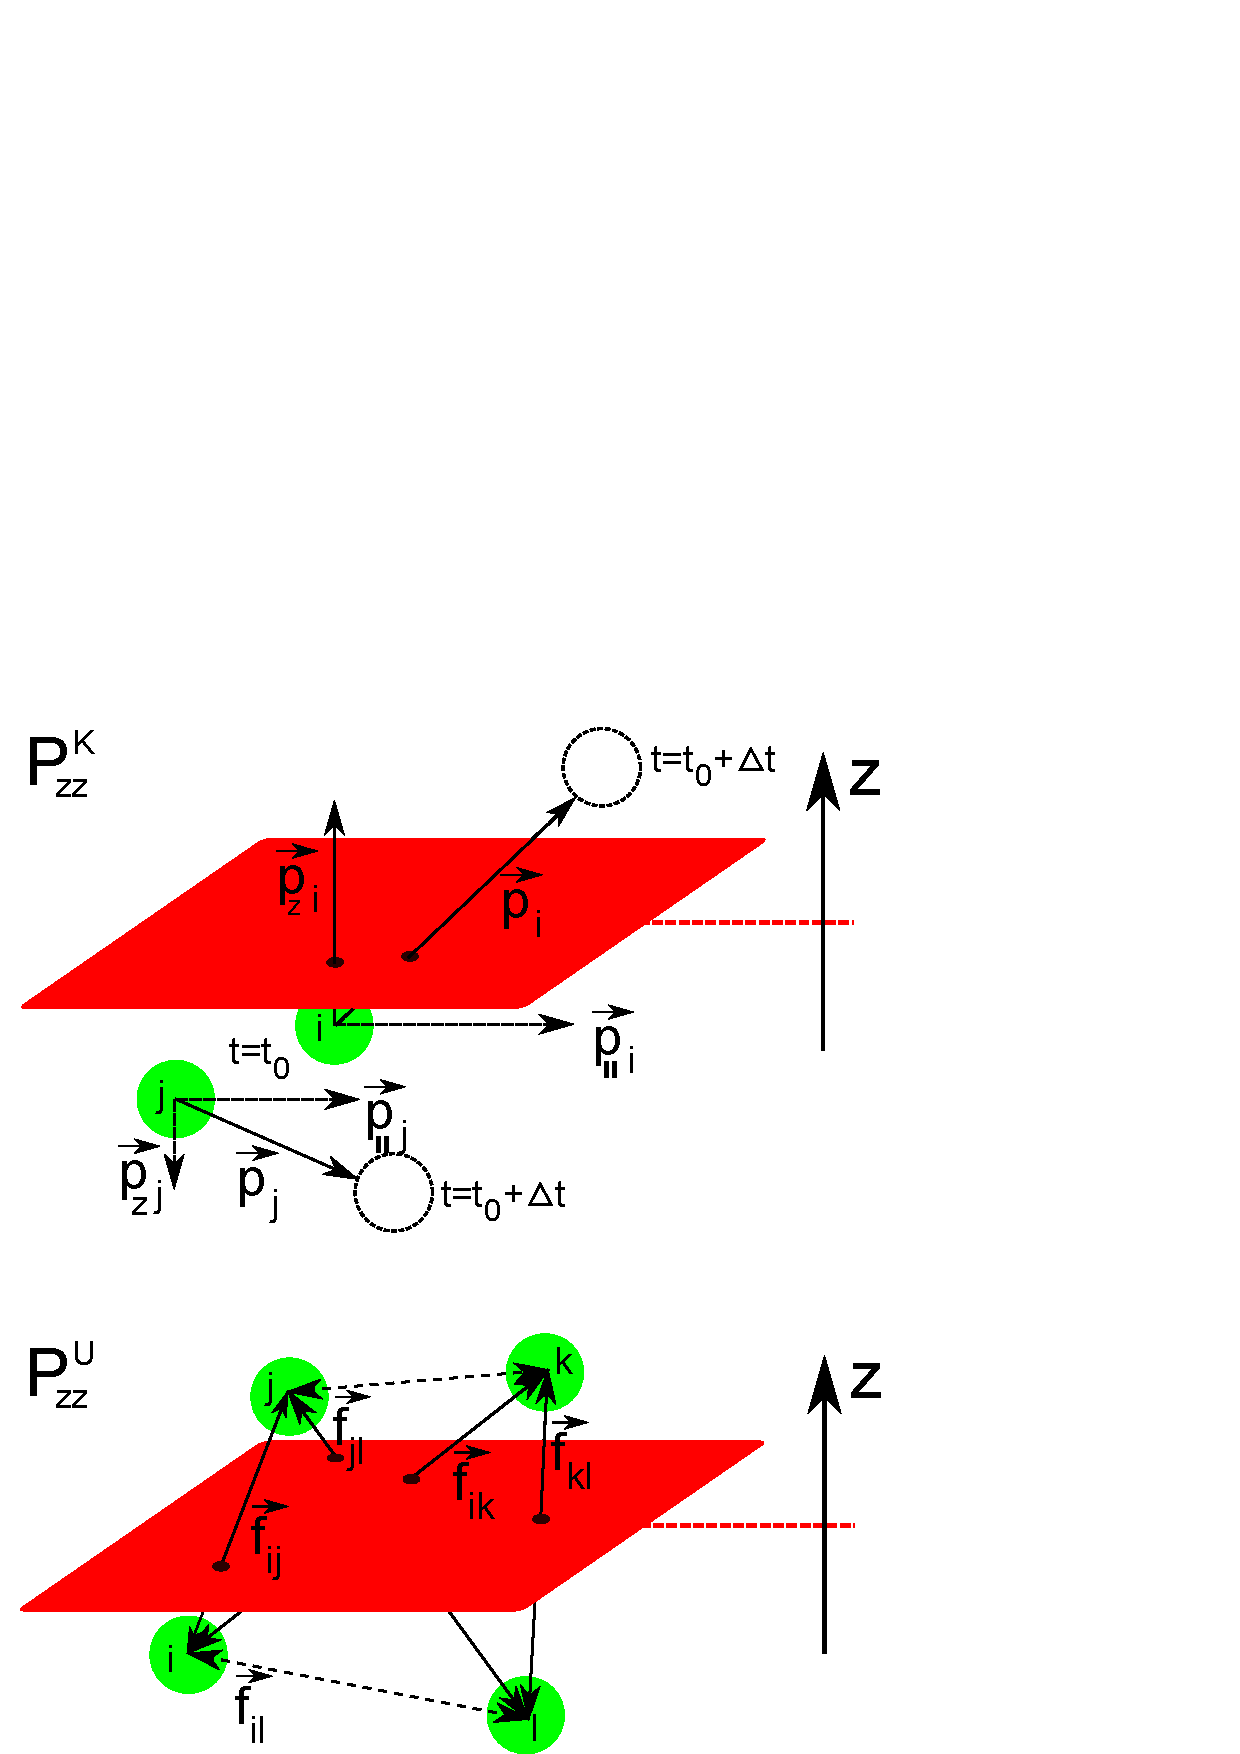
\includegraphics[width=60mm]{rysunki/cmst2.pdf}
\caption{Ilustracja sposobu obliczania kinetycznej (górny panel) i potencjalnej (dolny panel) składowej normalnej ciśnienia w metodzie MOP na podstawie wyrażeń (\ref{eq:mop1}) i (\ref{eq:mop2}).  Tylko oddziaływania dwucząsteczkowe (oznaczone jako ciągłe strzałki) wnoszą wkład do części potencjalnej $P_{zz}^{U}$ i tylko cząsteczki, które przekraczają płaszczyznę w danym kroku $dt$ wnoszą wkład do części kinetycznej $P_{zz}^{K}$.}
\label{cmst2}
\end{figure}
%
\\
Potencjalna część składowej $zz$ tensora ciśnienia w metodzie MOP wyraża się jako,
%
\begin{equation}
P_{zz}^{U}(z)= {1\over{4S}} \sum_{i} \sum_{j} F^{Z}_{ij} [ \Theta(z_{i}-z)\Theta(z-z_{j}) - \Theta(z_{j}-z)\Theta(z-z_{i})],
\label{eq:mop2}
\end{equation}
%
gdzie $\Theta$ oznacza funkcję Heaviside'a, natomiast $F^{Z}_{ij}$ jest $z$-tową składową siły między cząsteczkami $i$ i $j$. 
W powyższym wyrażeniu, rolą iloczynu z funkcją Heaviside'a jest wybranie
składnika siły międzycząsteczkowej, która przecina płaszczyznę. Wyraz $ij$ nie zmienia znaku przy zamianie z $i$ na $j$ (rysunek \ref{cmst2} ilustruje ten człon).
Gdyby układ był ograniczony atomami połączonymi za pomocą sprężyn do punktów wirtualnej sieci krystalicznej, wówczas oddziaływanie z nimi miałoby wkład do normalnej składowej ciśnienia
%
\begin{equation}
P_{zz}^{T}(z)=\pm {1 \over{S}} \sum_{i=1}^{N}
F^{e}_{z,i}\Theta(z_i-z)\Theta(z_m-z),
\label{eq:mop3}
\end{equation}
gdzie  $F^{e}_{z,i}$  oznacza $z$-ową składową siły zewnętrznej działającą na $i$-tą
cząsteczkę, $z$ to pozycja płaszczyzny MOP, natomiast $z_m$ oznacza pozycję środka
układu. Znak funkcji w równaniu (\ref{eq:mop3}) zależy od strony układu 
branej pod uwagę (+ dla dolnej części, - dla górnej części).
$P_{MOP}$ oznacza sumę wszystkich składników ciśnienia - część potencjalną,
kinetyczną oraz część związaną z działaniem ograniczających sprężyn. \\$P_{C}(z)=P_{zz}^{U}(z)+P_{zz}^{K}(z)$ to suma części potencjalnej i kinetycznej normalnej składowej ciśnienia.

Pomiędzy wieloma płaszczyznami, którymi można podzielić układ i względem których można liczyć wartość ciśnienia normalnego, dwie mają szczególne znaczenie. Są~to~płaszczyzny wyznaczone przez powierzchnię ograniczających ścian. Ich szczególność wiąże się z wykluczeniem możliwości wnikania cząsteczek ograniczonej części do wnętrza ścian. W związku z tym, zgodnie z definicją, kinetyczna część ciśnienia musi być równa zeru, natomiast wartość wypadkowego ciśnienia musi równać się potencjalnej części wyrażenia MOP. Wartość ciśnienia obliczonego w oparciu o potencjalną część wyrażenia MOP w sąsiedztwie ścian oznaczać będę symbolem $P_W$.  

Metodę płaszczyzn testowano w układzie o geometrii szczeliny. W celu odniesienia uzyskanych wyników do źródłowej pracy dotyczącej metody MOP \cite{Todd}, zdecydowano zbudować ściany ograniczające układ (obszary A i C) za pomocą sprężyn łączących cząsteczki do punktów wirtualnej sieci krystalicznej.
Wszystkie cząsteczki w układzie oddziaływały ze sobą potencjałem typu Weeks-Chandler-Anderson (WCA). Potencjał WCA jest krótkozasięgowym potencjałem odpychającym konstruowanym z potencjału LJ przez odcięcie w minimum $r_{cut} = r_{min} = 2^{1/6} \sigma$ i przesuniętym o $\epsilon$~\cite{AllenTildesley}.
%
Cząsteczki w ścianach (obszarach A i C) przyłączono do ustalonych punktów wirtualnej sieci krystalicznej potencjałem harmonicznym, $u(r_{i})= {1 \over 2} k_{2}(r_{i}-r_{0i})^{2}$,
gdzie $\underline{r}_{0i}$ jest pozycją $i$-tego węzła,
natomiast $k_{2}=57.15$ odpowiada stałej sprężystości sprężyny~\cite{Todd}. Ilustracje potencjałów stosowanych w rozprawie zawarto w dodatku \ref{oddzialywania}.
%
\begin{figure}[h]
\centering
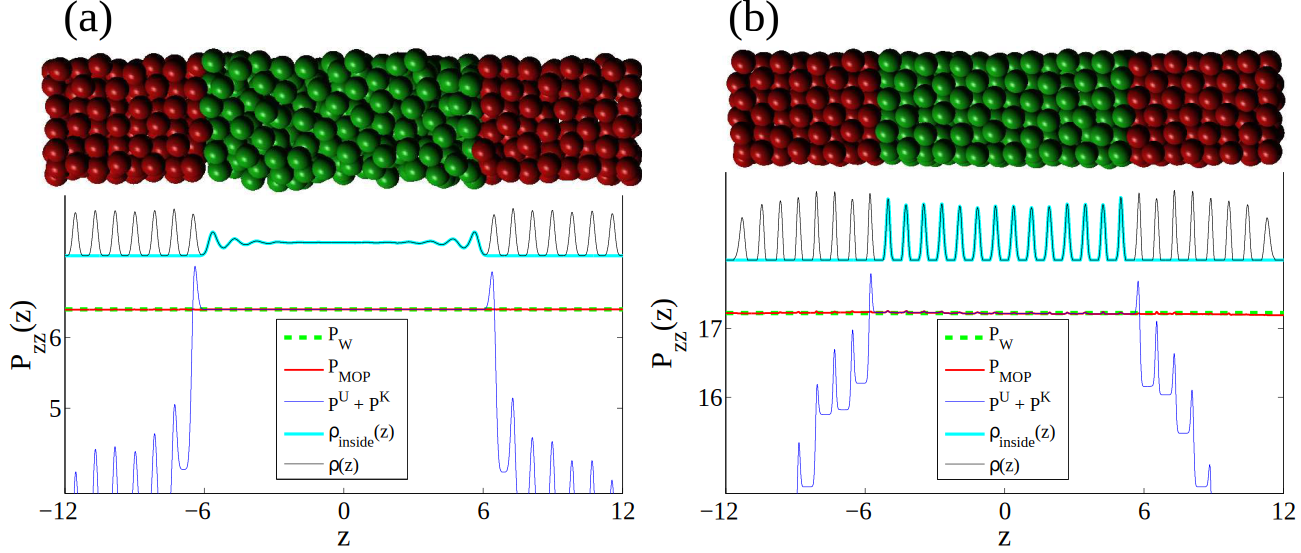
\includegraphics[width=150mm]{rysunki/PZZ.pdf}
\caption{Wyniki testu metody MOP dla układu szczeliny w stanie płynnym $\rho=0.8$ (panel a) oraz stanie stałym $\rho=1.1$ (panel b). Czerwona linia na wykresie przedstawia wartość ciśnienia MOP z uwzględnieniem wpływu sprężyn w ścianach. Linia niebieska oznacza sumę składowych potencjalnej i kinetycznej. Przerywana linia zielona reprezentuje wartość $P_{W}$ opartą na potencjalnej części wyrażenia MOP przy ścianie układu. Górne linie ciągłe przedstawiają całkowity (linia czarna) i wewnętrzny (linia jasnoniebieska) rozkład gęstości w całej szczelinie. W górnej części przedstawiono chwilową konfiguracje cząsteczek w danym stanie.}
\label{PZZ}
\end{figure}
%
Dobrane wartości parametrów oddziaływania wykluczają możliwość odejścia cząsteczek w ścianach od ich położeń równowagi na odległość większą niż 0.1 średniej odległości między nimi. Zapobiega to dyfuzji cząsteczek z obszaru B do obszarów A i C.
Wielkości fizyczne wyrażono w jednostkach zredukowanych t.j., odległość w $\sigma$, czas w $(m\sigma^{2}/k_{B}T)^{0.5}$, energia w $\epsilon$, natomiast masa atomowa $m$, była równa jedności. Obliczenia wykonano w temperaturze $T^{*}=k_{B}T/\epsilon =1$, gdzie $k_{B}$ jest stałą Boltzmanna. Związek pomiędzy jednostkami zredukowanymi a jednostkami SI (na przykładzie Argonu) został przedstawiony w dodatku \ref{redunit}. Ściany układu termostatowano za pomocą skalowania prędkości \cite{Woodcock1971}. 
%
Liczba cząsteczek w poszczególnych obszarach wynosiła odpowiednio $N_{A}=N_{C}=144$ i $N_{B}=252$. Obszar B był początkowo krystaliczny i składał się z czteroatomowych komórek FCC ustawionych w blok [$3\times 3 \times 7$]. Ściany A i C składały się z 4 warstw FCC (100) i były zbudowane z czteroatomowych komórek FCC ustawionych w blok [$3 \times 3 \times 4$]. \linebreak Równania ruchu całkowano algorytmem Verleta "skaczącej żaby" (dodatek \ref{algolnum}) przy użyciu kroku czasowego, $dt=0.0005$. \\
Badano układy w dwóch gęstościach odpowiadających płynowi $\rho=0.8$ oraz ciału stałemu $\rho=1.1$. 
%
%
Rysunek \ref{PZZ} przedstawia wyniki testu metody MOP dla układu w stanie płynnym $\rho=0.8$ oraz w stanie stałym $\rho=1.1$. 
%
%
Najważniejsze wnioski jakie można wyciągnąć z przeprowadzonych testów są następujące.
\begin{itemize}
\item{Wartość ciśnienia $P_W$ jest równa ciśnieniu obliczonemu zgodnie z wyrażeniem $P_{MOP}$ (ciśnienie wzdłuż kierunku $z$ ma stałą wartość).}
\item{W układach krystalicznych profil $P_{MOP}(z)$ (linia czerwona na rysunku \ref{PZZ}(b)) ujawnia niefizyczną strukturę (przekraczającą dopuszczalny słupek błędu), której maksima odpowiadają pozycjom warstw atomowych. Profil $P_{MOP}(z)$ nie jest linią gładką. Zostało to wyraźnie pokazane na rysunku \ref{PMOP-PW}(b) w postaci różnicy~$P_{MOP}(z)-P_W$.}
\end{itemize}
%
\begin{figure}[h]
\centering
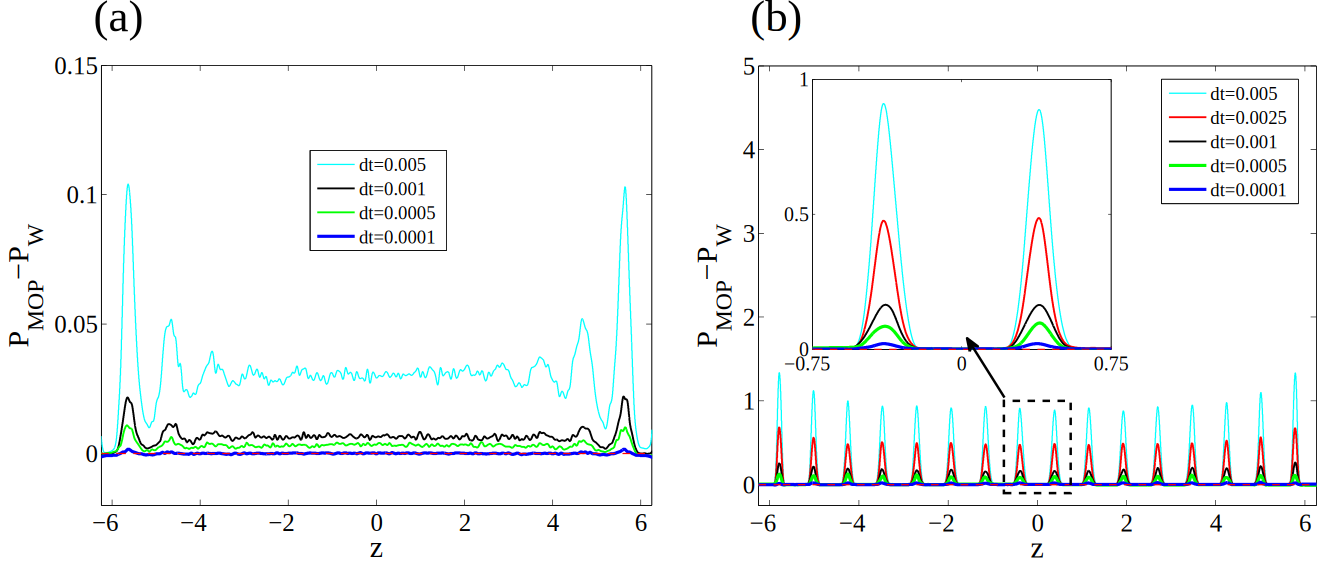
\includegraphics[width=150mm]{rysunki/PMOP-PW.pdf}
\caption{Różnica $P_{MOP}(z)-P_W$ w układzie w stanie płynnym (a) i stanie stałym (b), dla różnych wartości kroku czasowego $dt$, wzdłuż kierunku $z$. Ramka na rysunku (b) jest powiększeniem fragmentu głównego wykresu. W obu przypadkach spodziewanym wynikiem jest pozioma linia na wartości $P_{MOP}(z)-P_W=0$. Wartości różne od zera są związane z błędem generowanym przez kinetyczną część metody MOP, na co wskazuje wyraźna zależność od dobranego kroku czasowego $dt$.}
\label{PMOP-PW}
\end{figure}
%
Wyniki dodatkowych testów przedstawiono na rysunku \ref{PMOP-PW}. 
%
%
Podobnie jak w przypadku rysunku \ref{PZZ}, panel (a) odpowiada układowi w stanie płynu ($\rho=0.8$), natomiast panel (b) układowi krystalicznemu ($\rho=1.1$). Rysunek \ref{PMOP-PW} przedstawia różnicę między \linebreak ciśnieniem $P_{MOP}$ a $P_W$ wzdłuż kierunku $z$. Dodatkowo, testy wykonano dla różnych wartości kroku czasowego. Ponieważ ciśnienie $P_W$ jest obliczane w miejscu, gdzie cząsteczki nie mogą przejść przez płaszczyznę (względem której prowadzone są obliczenia), różnica $P_{MOP}(z)-P_W$ powinna być równa zeru wzdłuż całego układu. Okazuje się jednak, że ta różnica nie jest równa zeru, a jej wartość zależy od dobranego kroku czasowego. W przypadku stanu płynnego (rysunek \ref{PMOP-PW}(a)) efekt ten jest trudno zauważalny (wartość różnicy nie przekracza 0.1 zredukowanej jednostki ciśnienia przy kroku czasowym $dt=0.005$). Największym błędem jest obarczona część profilu bliska ścianom układu. W~przypadku układu w stanie stałym (rysunek \ref{PMOP-PW} (b)) odchylenie różnicy $P_{MOP}(z)-P_W$ od zera jest bardziej widoczne, a jej wartość jest o rząd wielkości większa (dla kroku czasowego $dt=0.005$, różnica wynosi około 1 zredukowaną jednostkę ciśnienia). Warto zaważyć, że w obu przypadkach różnica $P_{MOP}(z)-P_W$ zmierza do zera wraz ze zmniejszaniem kroku czasowego $dt$. Otrzymane wyniki każą sądzić, że problem niezerowej różnicy $P_{MOP}(z)-P_W$ w układzie musi mieć przyczyny numeryczne. W symulacjach MD równania ruchu całkuje się często stosując stały krok czasowy $dt$.
Część potencjalna i kinetyczna jest wyliczana w dyskretnych chwilach czasu, $ndt$ gdzie $n=1,2,...~$. Cząsteczki jednak przekraczają płaszczyznę w chwilach, $t_{i,m}$ które są zwykle pomiędzy, zamiast w całkowitych wielokrotnościach $dt$, co ma wkład do kinetycznej części wyrażenia MOP. Aby uzyskać dokładne wyniki ciśnienia $P_{MOP}$ wymagane jest stosowanie dostatecznie małego kroku czasowego $dt$. 

%
%
Przedstawione obliczenia prezentują główny problem związany ze stosowaniem metody MOP. Obliczając ciśnienie metodą MOP w niejednorodnie ograniczonych układach cząsteczek należy pamiętać o problemach związanych z dokładnym obliczaniem kinetycznej części ciśnienia, w szczególności w układach o dużej gęstości. Polegają one na trudności określenia chwili, w której cząsteczki przechodzą na drugą stronę płaszczyzny obliczeniowej. Pokazuje to zależność kinetycznej części $P_{MOP}$ od kroku czasowego $dt$ (rysunek \ref{PMOP-PW}). Obliczenia pokazują, że w płaszczyźnie przy ścianie ograniczającej układ, wartość ciśnienia $P_{MOP}$ jest równa ciśnieniu $P_W$.  W praktyce, rozsądna redukcja kroku czasowego, wystarcza, aby zapewnić dostateczną dokładność obliczania ciśnienia MOP. Niemniej obliczanie ciśnienia $P_W$ (część potencjalna ciśnienia $P_{MOP}$ przy ścianie ograniczającej układ) zamiast $P_{MOP}$ jest rozwiązaniem prostszym i bardziej efektywnym obliczeniowo.
W dalszej części pracy, chwilowe ciśnienie normalne będzie obliczane w~oparciu o potencjalną część wyrażenia MOP przy ścianie ograniczającej układ. Można ją równoważnie przedstawić jako całkowitą wartość $z$-owej składowej siły z jaką cząsteczki ograniczonej części działają na ścianę układu, $P_W=F_z / S$ (gdzie $S$ jest polem przekroju układu w płaszczyźnie $xy$).
%UWAGI: napisać o zastosowanym barostacie oraz jak ścinano układ. Zacytować Petravic, Heyesa, Butlera-Harowella.
\section{Kontrola ciśnienia}
\label{barostaty}
%
Kontrola ciśnienia w symulacjach MD wymaga zastosowania tzw. barostatu - dodatkowego mechanizmu nałożonego na równania ruchu, odpowiedzialnego za doprowadzenie i utrzymanie układu w stanie o ustalonej wartości ciśnienia. W symulacjach układów silnie ograniczonych, kontrola ciśnienia nie jest zagadnieniem w pełni rozwiązanym. Wiele badań prowadzono w warunkach stałej odległości między ścianami \cite{hartkamp,LiemBrownClarke}. Jednak w~wielu układach tribologicznych realizują się warunki stałego ciśnienia, a nie objętości \cite{ponjavic14, spikes06}. W ramach rozprawy doktorskiej przebadano dotychczasowe schematy kontroli ciśnienia i zaproponowano nowe. Badane barostaty można podzielić na dwie kategorie. Pierwsza, to {barostaty globalne} (BG), natomiast druga to {barostaty mikroskopowe} (BM). W tej części zostaną omówione najważniejsze aspekty barostatów globalnych i~mikroskopowych.
\subsection{Barostaty globalne}
\label{barostaty_globalne}
Schemat działania barostatów globalnych przedstawia rysunek \ref{BG-schemat}.
%
\begin{figure}[h]
\centering
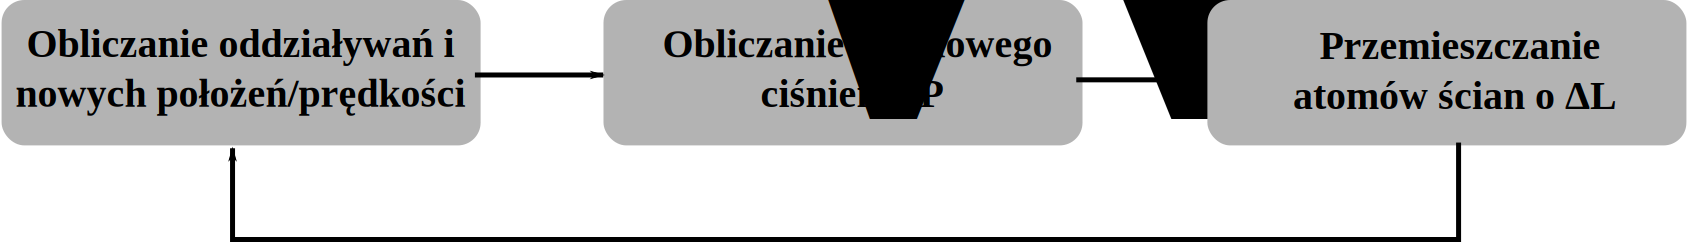
\includegraphics[width=160mm]{rysunki/BG-schemat.pdf}
\caption{Ilustracja działania barostatów globalnych w symulacji MD.}
\label{BG-schemat}
\end{figure}
%
%
%
%
%
%
Układ cząsteczek realizuje równania ruchu (z termostatem lub bez termostatu). Po każdym kroku czasowym, w układzie jest obliczane ciśnienie chwilowe. Następnie, na podstawie informacji o różnicy pomiędzy wartością chwilowego ciśnienia $P_{int}(t)$, a zadaną wartością ciśnienia $P_N$, ściany układu są do siebie zbliżane lub oddalane, zgodnie z rozwiązaniem równania barostatu. Przebadano barostaty globalne opisane następującymi równaniami: \\
\\
A) barostat Butlera-Harrowela (BG-A)\cite{ButlerHarrowell2003}\\
\begin{equation}
\dot{L}= \tau (P_W(t)-P_N),
\label{BGA}
\end{equation}
\\
B) barostat Lupkowskiego-van Swalla (BG-B)\cite{LupowskivanSwoll91a, LupowskivanSwoll91b}\\
\begin{equation}
\ddot{L}= \tau (P_W(t)-P_N),
\label{BGB}
\end{equation}
\\
C) barostat Pastewki-Heyesa (BG-C)\cite{Pastewka2010, Gattinoni2014},\\
\begin{equation}
\ddot{L}= \tau^2 (P_W(t)-P_N) -2 \tau \dot{L}.
\label{BGC}
\end{equation}
\\
Barostaty (BG-A) i (BG-B) były stosowane wcześniej \cite{LupowskivanSwoll91a, LupowskivanSwoll91b, ButlerHarrowell2003, DMH1, Gattinoni2013}, natomiast barostat (BG-C) został częściowo zaproponowany w przeprowadzonych przez doktoranta badaniach \cite{Gattinoni2014}. 
Barostat (BG-C) można traktować jako modyfikację barostatu (BG-B).
Zastosowanie barostatów globalnych wiąże się z dwoma problemami.
Pierwszym jest obliczanie ciśnienia w układzie. Informacja o ciśnieniu jest wielkością wejściową w schemacie kontroli ciśnienia. Błąd lub znaczna niedokładność w jej wyznaczaniu może wiązać się z niefizycznym zaburzeniem układu. 
%
Drugą trudnością jest dobór stałej sprzężenia zwrotnego $\tau$. Każdy z wymienionych schematów zawiera w sobie czynnik odpowiedzialny za sprzężenie pomiędzy układem a barostatem. W ramach badań opracowano procedurę doboru tej stałej. Dobór stałej sprzężenia zwrotnego jest zagadnieniem istotnym, ponieważ nieodpowiednia wartość stałej może wprowadzić układ w zakres niefizycznych zachowań, a w skrajnych wypadkach, do rezonansu układ-barostat i dezintegracji całego układu. 
%
Problem obliczania ciśnienia został omówiony w sekcji \ref{cisnienie}. 
Odnosząc się do problemu doboru stałej $\tau$, w pierwszej kolejności należy odpowiedzieć na pytanie, jak powinien zachowywać się układ o właściwie dobranej stałej sprzężenia? Dobrze dobrana stała 1)~nie powinna prowadzić układu do rezonansu z barostatem, 2)~wyniki fizyczne, w~pewnym zakresie wartości stałej, nie powinny być od niej zależne, oraz 3)~układ powinien być prowadzony do zadanej wartości ciśnienia w możliwie krótkim czasie. Zastosowano następującą procedurę doboru stałej sprzężenia zwrotnego.%
\begin{figure}
\centering
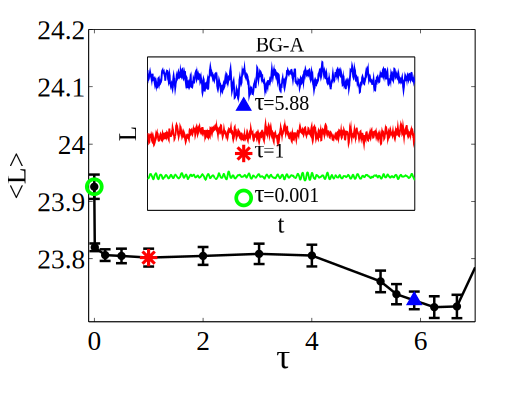
\includegraphics[width=100mm]{rysunki/BG-A.pdf}
\caption{Średnia szerokość układu $\langle L \rangle$ w zależności od wartości stałej sprzężenia zwrotnego $\tau$, dla barostatu (BG-A). Na wykresie zaznaczono słupki błędu. Wstawiona ramka przedstawia czasowe przebiegi $L(t)$ dla wybranych wartości stałej $\tau$.}
\label{wykBG-A}
\end{figure}
\begin{figure}
\centering
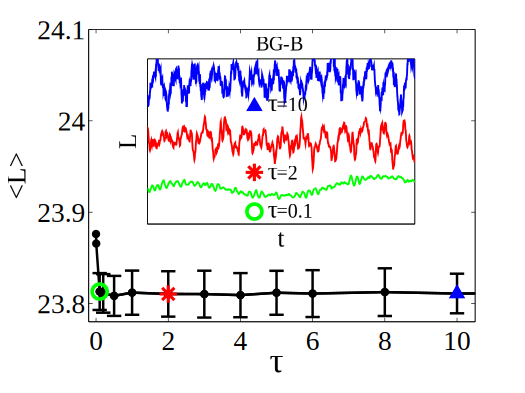
\includegraphics[width=100mm]{rysunki/BG-B.pdf}
\caption{Jak dla rysunku \ref{wykBG-A}, ale dla barostatu (BG-B). Wstawiona ramka przedstawiająca zależność $L(t)$ wskazuje, że bez względu na dobór stałej $\tau$, w układzie pojawiają się drgania.}
\label{wykBG-B}
\end{figure}
\begin{figure}
\centering
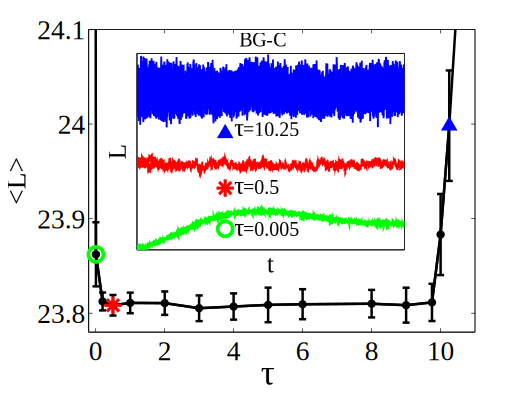
\includegraphics[width=100mm]{rysunki/BG-C.pdf}
\caption{Jak dla rysunku \ref{wykBG-A} oraz \ref{wykBG-B}, ale dla barostatu (BG-C).}
\label{wykBG-C}
\end{figure}
%
\begin{samepage}
Pośród wielu wielkości fizycznych, na których zachowanie może mieć wpływ stała sprzężenia, analizie poddano średnią szerokość układu $\langle L \rangle$. Szerokość układu $L$ ma prostą definicję (dystans między środkami mas ścian), jej wartość reguluje równanie barostatu i bezpośrednio wpływa na~ciśnienie w układzie. Następnie sprawdzono jak wartość $\langle L \rangle$ oraz rozkład chwilowych wartości $L(t)$ zależy od zadanej wartości stałej sprzężenia $\tau$. Rysunki \ref{wykBG-A}, \ref{wykBG-B}, \ref{wykBG-C}, przedstawiają zależności $\langle L \rangle$ od wartości $\tau$ dla kolejnych barostatów. \linebreak Wyniki w ramkach na rysunkach \ref{wykBG-A}, \ref{wykBG-B}, \ref{wykBG-C} przedstawiają przykładowe przebiegi czasowe $L(t)$. 
\end{samepage}
%
%
%


Wszystkie testowane barostaty posiadają zakres wartości $\tau$, w którym $\langle L \rangle$ ma stałą wartość. Mimo tego, w przypadku barostatu (BG-B) (rysunek \ref{wykBG-B}) układ jest wprowadzany w drgania, niezależnie od doboru stałej $\tau$, co ujawnia ramka czasowych przebiegów $L(t)$. W przypadków barostatów (BG-A) i (BG-C) (rysunki \ref{wykBG-A} i \ref{wykBG-C}) oscylacje wielkości $L(t)$ pojawiają się tylko dla bardzo małych bądź bardzo dużych wartości $\tau$. Dla wartości w środkowym zakresie przedziału oscylacje układu są zaniedbywalne.   

Również rysunek \ref{BG-rozklad-skok}(a), który przedstawia rozkład wielkości $L(t)$ wskazuje, \linebreak że w przypadku barostatu (BG-B) uzyskany rozkład znacznie odbiega od pozostałych i nie można znaleźć takiej wartości stałej $\tau$, dla której otrzymany rozkład pokrywałby się z rozkładami szerokości szczeliny $P(L)$ dla pozostałych barostatów. 

%
%
Ostatnim testem, jaki wykonano w odniesieniu do barostatów globalnych, było sprawdzenie odpowiedzi barostatów (BG-A), (BG-B) i (BG-C) na zmianę zadanego ciśnienia. Odpowiedź ilustruje przebieg $L(t)$.
%
\begin{figure}[h]
\centering
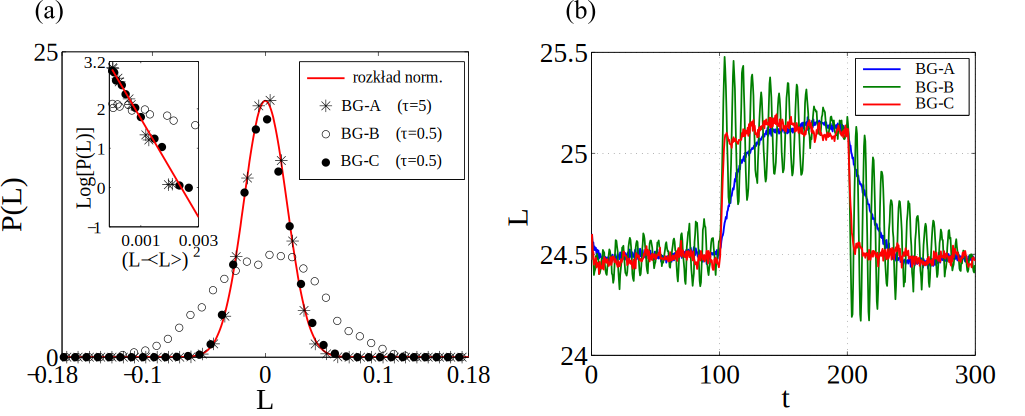
\includegraphics[width=160mm]{rysunki/BG-rozklad-skok.pdf}
\caption{Rozkład szerokości szczeliny $L$ dla wybranej wartości stałej $\tau$ (panel~a), oraz test odpowiedzi układu na jednostkową zmianę docelowego ciśnienia (panel b) dla barostatów (BG-A), (BG-B), (BG-C).}
\label{BG-rozklad-skok}
\end{figure}
%
Uzyskane wyniki są przedstawione na rysunku \ref{BG-rozklad-skok}(b). Widać, że barostat B wywołuje pojawienie się drgań w układzie. Barostat A nie wywołuje drgań, ale zachowanie najbliższe pożądanemu wykazuje barostat C, który nie wywołuje drgań oraz prowadzi układ do wartości $L$ (odpowiadającej zadanemu ciśnieniu~$P_N$) w~ najkrótszym~czasie. 
%
%
% 
\subsection{Barostat mikroskopowy}
%
Tematem poprzedniego rozdziału były globalne schematy kontroli ciśnienia, których działanie opierało się na nałożeniu na równania ruchu cząsteczek ścian dodatkowego (zewnętrznego) równania. W tej części zostanie omówiona drugi rodzaj schematów kontroli ciśnienia - barostat mikroskopowy. BM opiera się na działaniu dodatkowej siły na poszczególne cząsteczki ścian. Dla układu o geometrii zgodnej z ilustracją na rysunku \ref{szczelina}, równania ruchu z członem kontrolującym ciśnienie mają następującą postać:%
\\
dla obszaru A,
%
\begin{equation}
\begin{gathered}
\underline{\dot{r}}^A_i=\underline{p}^A_i/m_i^A,
%
\\
%
\underline{\dot{p}}^A_i=\underline{F}^{AA}_i +
\underline{F}^{AB}_i +
\underset{\text{ }}{\Bigg\{ \underline{F}^{exA}_i + b \left(\frac{\mathbb{P}^z_A}{M_A} - \frac{\mathbb{P}^z_C}{M_C} \right) \hat{\underline{z}} \Bigg\}},
\label{eq:b2}
\end{gathered}
\end{equation}
%
dla obszaru B,
%
\begin{equation}
\begin{gathered}
\underline{\dot{r}}^B_k=\underline{p}^B_k/m_k^B,
\\
\underline{\dot{p}}^B_k=\underline{F}^{BA}_k +
\underline{F}^{BB}_k + \underline{F}^{BC}_k,
\label{eq:b4}
\end{gathered}
\end{equation}
%
dla obszaru C,
%
\begin{equation}
\begin{gathered}
\underline{\dot{r}}^C_l=\underline{p}^C_l/m_l^C,
\\
\underline{\dot{p}}^C_l=\underline{F}^{CC}_l +
\underline{F}^{CB}_l +
\underset{\text{ }}{\Bigg\{ \underline{F}^{exC}_l - b \left( \frac{\mathbb{P}^z_A}{M_A} - \frac{\mathbb{P}^z_C}{M_C} \right) \hat{\underline{z}} \Bigg\}},
\label{eq:b6}
\end{gathered}
\end{equation}
%
gdzie $\underline{F}^{AA}_i, \underline{F}^{AB}_i, \underline{F}^{BA}_k, \underline{F}^{BB}_k, \underline{F}^{BC}_k, \underline{F}^{CC}_l, \underline{F}^{CB}_l$ to siły wzajemnego oddziaływania między cząsteczkami w obszarach oznaczonych przez A, B, C, symbole $M_A, M_C$ oznaczają masy ścian ograniczających układ, które można wyrazić jako $M_A=\sum_{i}^{N_A}{m_i}, M_C=\sum_{l}^{N_C}{m_l}$, natomiast $\underline{F}_i^{exA}, \underline{F}_i^{exC},$ to siły związane z zewnętrznym (zadanym) ciśnieniem. Ich wartość jest równa $F_i^{exA}=F_i^{exC}=P_N S/N_A=P_N S/N_C$. $b \left( \frac{\mathbb{P}^z_A}{M_A} - \frac{\mathbb{P}^z_C}{M_C} \right)$ to wyraz odpowiedzialny za tłumienie. Wartość wyrazu tłumiącego jest proporcjonalna do względnej prędkości ścian w kierunku działania barostatu. 

Można zauważyć, że jeśli szerokość układu $L$ zostanie zdefiniowana jako odległość między środkami masy $L=(\underline{\mathbb{R}}_A - \underline{\mathbb{R}}_C) \cdot \underline{\hat{z}}$, natomiast masy ścian będą mieć tą samą wartość $M_W$, to wykonując dwukrotne różniczkowanie po czasie otrzymujemy wyrażenie\\
\begin{equation}
\ddot{L}=\frac{2S}{M_W}(P_W(t)-P_N) - 2b \dot{L}.
\end{equation}
%
Przyjmując $b=\sqrt{S/2M_W}$ oraz $\tau=2b$, otrzymujemy $\ddot{L}=\tau^2 (P_W(t)-P_N) - \tau \dot{L}$. Postać otrzymanego równania na $\ddot{L}$ jest identyczna jak równanie barostatu globalnego (BG-C)~(równanie \ref{BGC}), natomiast gdy stała tłumienia $b=0$, otrzymujemy równanie postaci odpowiadającej barostatowi globalnemu (BG-B)~(równanie \ref{BGB}). 

Dla opracowanego schematu kontroli ciśnienia przeprowadzono analogiczne testy do tych, przedstawionych w rozdziale \ref{barostaty_globalne}. Sprawdzono zależność otrzymywanych wyników średniej szerokości układu $\langle L \rangle$ od wartości stałej $b$, rozkład wielkości $L(t)$ oraz odpowiedź układu na zmianę zadanej wartości ciśnienia $P_N$. Rysunek \ref{BM-L-of-t} przedstawia zależność $\langle L \rangle$ dla różnych wartości stałej $b$.
\begin{figure}[h]
\centering
\includegraphics[width=100mm]{rysunki/PRE14_fig7.pdf}
\caption{Zależność średniej szerokości szczeliny $\langle L \rangle$ od wartości stałej $b$ dla barostatu mikroskopowego. Ramka przedstawia chwilowe przebiegi $L(t)$.}
\label{BM-L-of-t}
\end{figure}
Otrzymane wyniki wskazują małą zależność $\langle L \rangle$ od~wartości~$b$. Warto zauważyć, że tylko w sytuacji $b=0$, przebiegi czasowe przedstawione w ramce ujawniają oscylacje w przebiegu $L(t)$. Gdy $b=0$, schemat staje się odpowiednikiem barostatu (BG-B) (dla którego również obserwowano oscylacje $L(t)$). 

Rysunek \ref{BM-rozklad-skok}(a) przedstawia rozkład wielkości $L(t)$ dla różnych wartości stałej $b$. Podobnie jak w przypadku wyników przedstawionych na rysunku \ref{BM-L-of-t}, widać, że gdy stała tłumienia $b=0$ rozkład $L(t)$ odbiega od spodziewanego trendu. Rysunek \ref{BM-rozklad-skok}(b) przedstawia odpowiedź układu na zmianę wartości przyłożonego ciśnienia $P_N$.
\begin{figure}[h]
\centering
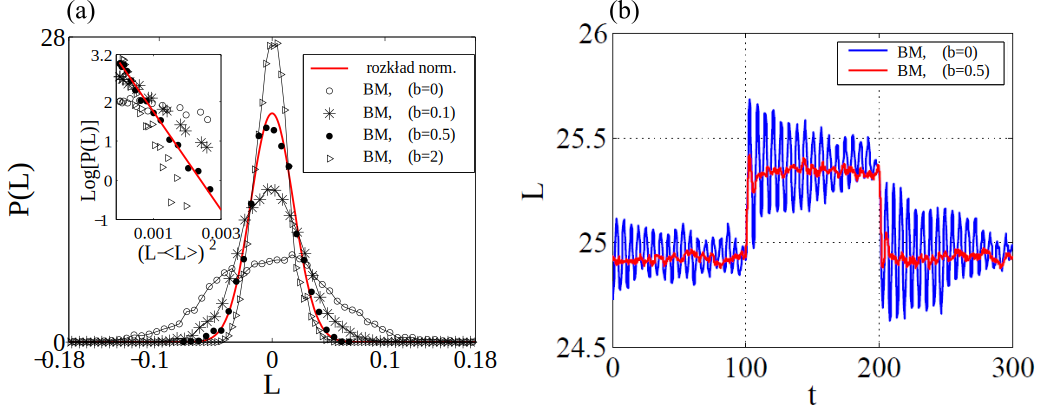
\includegraphics[width=160mm]{rysunki/BM-rozklad-skok.pdf}
\caption{Rozkład $L(t)$ dla różnych wartości stałej $b$ (panel a) oraz odpowiedź układu na skokową zmianę zadanego ciśnienia$P_N$ (panel b).}
\label{BM-rozklad-skok}
\end{figure}
%
Gdy stała tłumienia $b=0$ układ odpowiada znacznymi oscylacjami w trakcie zmiany zadanego ciśnienia. Występujące oscylacje są konsekwencją sposobu kontroli ciśnienia bez mechanizmu tłumienia drgań. Układ zachowuje się podobnie jak w przypadku barostatu~(BG-B). Gdy wartość stałej tłumienia $b=0.5$, barostat prowadzi układ do zadanego stanu w sposób zgodny z oczekiwaniami (brak oscylacji, szybka reakcja układu na zmianę wartości $P_N$). W porównaniu do barostatów globalnych, kontrola ciśnienia za pomocą schematu mikroskopowego ma następujące zalety:
\begin{itemize}
\item{brak konieczności obliczania wartości ciśnienia w układzie, }
%\item{brak stałej sprzężenia zwrotnego w schemacie,}
\item{nieznaczna zależność wyników od wartości stałej tłumienia $b$,}
\item{kontrola ciśnienia opiera się na wprowadzeniu do równań ruchu dodatkowych sił, które można interpretować jako zewnętrzne obciążenie układu,}
\item{zaproponowane równania zachowują pęd całkowity układu.}
\end{itemize}
%
%
%
\section{Kontrola ścinania}
\label{shearostat}
%
Modelowanie tarcia wymaga rozbudowy algorytmu o możliwość kontroli ścinania. W~przypadku układu o geometrii zgodniej z ilustracją na rysunku \ref{szczelina}, kierunkiem ścinania jest kierunek $x$. W układach ograniczonych cząsteczkami połączonymi za pomocą sprężyn z węzłami wirtualnej sieci, ścinanie można realizować poprzez przesuwanie pozycji węzłów sieci (bądź zarówno węzłów i atomów ścian) w każdym kroku czasowym $dt$ o dystans $d s=v_0 d t$ \cite{DMH1}. Ścinanie można również wywołać przykładając siły styczne do powierzchni ścian układu. W związku z tym, do równań ruchu wprowadzono wyraz reprezentujący siły ścinające. 

%
\subsection{Równania ruchu}
\label{rownania_ruchu_scinania}
%
Aby wprowadzić i kontrolować w układzie siły styczne, do równań ruchu cząsteczek w ścianach, dodano wyraz reprezentujący działanie siły zależnej od różnicy pomiędzy chwilową, względną prędkością ścian, a prędkością zadaną. Równania ruchu dla układu mikroszczeliny z kontrolowaną wartością siły stycznej mają postać\\
dla obszaru A,
%
\begin{equation}
\begin{gathered}
\underline{\dot{r}}^A_i=\underline{p}^A_i/m_i^A,
%
\\
%
\underline{\dot{p}}^A_i=\underline{F}^{AA}_i +
\underline{F}^{AB}_i  +
\underset{\text{}}{\Bigg\{ \gamma \left( \left| \frac{\mathbb{P}^x_A}{M_A} - \frac{\mathbb{P}^x_C}{M_C} \right| - 2v_0 \right) \hat{\underline{x}} \Bigg\}},
\label{eq:sh2}
\end{gathered}
\end{equation}
%
dla obszaru B,
%
\begin{equation}
\begin{gathered}
\underline{\dot{r}}^B_k=\underline{p}^B_k/m_k^B,
\\
\underline{\dot{p}}^B_k=\underline{F}^{BA}_k +
\underline{F}^{BB}_k + \underline{F}^{BC}_k,
\label{eq:sh4}
\end{gathered}
\end{equation}
%
dla obszaru C,
%
\begin{equation}
\begin{gathered}
\underline{\dot{r}}^C_l=\underline{p}^C_l/m_l^C,
\\
\underline{\dot{p}}^C_l=\underline{F}^{CC}_l +
\underline{F}^{CB}_l -
\underset{\text{}}{\Bigg\{ \gamma \left( \left| \frac{\mathbb{P}^x_A}{M_A} - \frac{\mathbb{P}^x_C}{M_C} \right| - 2v_0 \right) \hat{\underline{x}} \Bigg\}},
\label{eq:sh6}
\end{gathered}
\end{equation}
%
gdzie $\mathbb{P}^x_A, \mathbb{P}^x_C$ to całkowite pędy ścian A i C w kierunku $x$, $v_0$ to docelowa prędkość ścinania, natomiast $\gamma$ to stała sprzężenia układu z członem ścinającym. Siła jaka działa na ściany układu, jest proporcjonalna do różnicy pomiędzy względną prędkością ścian $\left| \frac{\mathbb{P}^x_A}{M_A} - \frac{\mathbb{P}^x_C}{M_C} \right|$, a docelową prędkością ścinania $2 v_0$. Kiedy układ osiąga zadaną prędkość ścinania, siła również maleje do zera. W ten sposób człon ścinający działa na układ dokładnie taką siłą, jaka jest potrzebna aby uzyskać stałą prędkość poślizgu.
\begin{figure}[h]
\centering
\includegraphics[width=160mm]{rysunki/v_od_gamma.pdf}
\caption{Zależność $v(t)$ (główna część wykresu) oraz $\langle v \rangle(\gamma)$ (ramka) dla układu w stanie płynnym (a) i stałym (b). Kolejne kolory linii i znaczników oznaczają kolejne wartości stałej $\gamma$. Panel (a) pokazuje, że w stanie płynnym, już przy wartości $\gamma=10$ w~układzie realizuje się ścinanie z prędkością równą prędkości zadanej. W przypadku ciała stałego (panel b), ścinanie z prędkością równą prędkości ścinania pojawia się dopiero od wartości $\gamma=50$.}
\label{v_od_gamma}
\end{figure}
Jednym z testów jakie wykonano w odniesieniu do zaproponowanej metody, było sprawdzenie wpływu stałej $\gamma$ na uzyskaną prędkość ścinania układu. Naturalnym pytaniem, które pojawia się w odniesieniu do nowej metody, dotyczy doboru stałej $\gamma$ bądź jej wpływu na~wyniki symulacji. Rysunek \ref{v_od_gamma} przedstawia uzyskane przebiegi $v(t)$ dla różnych wartości $\gamma$ oraz zależności $\langle v \rangle(\gamma)$ dla układu w stanie płynnym (a) i stanie stałym (b).

%
W układzie w stanie płynnym (rysunek \ref{v_od_gamma}(a)) prawie każda wartość $\gamma$ wywołuje ścinanie, ale ścinanie z prędkością względną równą wartości zadanej $ v_0$ uzyskano dopiero dla $\gamma>0.1$. W układzie w stanie stałym (rysunek \ref{v_od_gamma}(b)) widać z kolei, że prędkość równą zadanej wartości $v_0$, układ osiąga dopiero, gdy $\gamma=50$. Dla mniejszych wartości $\gamma$ ścinanie nie zachodzi (np. dla $\gamma=5$) lub zachodzi, ale z prędkością dużo mniejszą od~$v_0$. Można sądzić, że wartość $\gamma$ musi być wyższa od pewnej granicznej wartości.
%
\subsection{Prędkość względna w ujęciu modelu Petravic}
%
Metoda ścinania przedstawiona w poprzedniej sekcji (\ref{rownania_ruchu_scinania}) polega na przyłożeniu do ścian układu siły proporcjonalnej do różnicy pomiędzy aktualną wartością względnej prędkości ścian a prędkością docelową $2v_0$. Gdy ściany mają równe masy, każda z nich przemieszcza się średnio z tą samą wartością prędkości, ale przeciwnie skierowaną. Ze~względu na złożony charakter oddziaływania z ograniczoną częścią układu, chwilowe prędkości górnej i dolnej ściany nie są~sobie równe, niemniej siły działające na ściany są sobie równe i przeciwnie skierowane w każdym kroku, co skutkuje zachowaniem zerowego pędu całkowitego. Środek masy również jest zachowany.

Zastosowanie względnej prędkości pomiędzy ścianami w zaproponowanych równaniach ruchu może być dyskutowane w oparciu o konkluzje Petravic \cite{Petravic2}, dotyczące przyczyn tarcia działającego na cząsteczkę w skończonej objętości płynu. Pokazano, że fluktuacyjne wyrażenie na współczynnik tarcia ruchomej, masywnej cząsteczki w płynie o~skończonej objętości (lub masie) wraz z upływem czasu dąży do zera. Dzieje się tak, ponieważ cząsteczka wprawia w ruch cały otaczający ją ośrodek, w związku z czym względna prędkość cząsteczki i płynu zmierza do zera. Petravic postuluje zależność tarcia od względnej (a nie absolutnej) prędkości cząsteczki i płynu. Aby siła tarcia była stała w czasie, należy rozważać względny ruch dwóch nieskończonych mas (w tym przypadku cząsteczka o nieskończonej masie miałaby poruszać się względem płynu w nieskończonej objętości). 

Rozważmy cząsteczkę o skończonej masie $m$, poruszającą się w lepkim płynie o nieskończonej objętości. W tym przypadku siła tarcia ostatecznie zbiega do zera w czasie~$t$. Związek pomiędzy całkowitą siłą działającą na cząsteczkę $F_T(t)$, a przyspieszeniem cząsteczki można zapisać jako $a(t)=dv(t)/dt=F_T(t)/m$, gdzie $F_T(t)$ jest sumą siły wymuszającej $F_d(t)$ i siły tarcia $F_f(t)$. Załóżmy, że siła tarcia $F_f(t)$ jest proporcjonalna do względnej prędkości pomiędzy cząsteczką oraz otaczającym płynem, tzn. $F_f(t)=-\eta v(t)$, gdzie $\eta$ jest współczynnikiem tarcia wewnętrznego (lepkości ośrodka) i ma stałą wartość. Jeżeli w układzie nie ma siły wymuszającej $F_d(t)$, przyspieszenie cząsteczki sprowadza się do $a(t)=-v(t)\eta / m$, natomiast prędkość cząsteczki zbiega do zera. Aby zachować stałą prędkość cząsteczki w układzie, tzn. $v(t) \to v_0$ (lub równoważnie $a(t) \to 0$), masa cząsteczki musi być nieskończona \cite{Petravic2}. Taki sam wynik można uzyskać w sytuacji gdy całkowita siła działająca na cząsteczkę dąży do zera, tzn. $F_T(t) \to 0$. Stałą prędkość średnią można uzyskać przez przyłożenie siły wymuszającej spełniającej warunek $F_d(t) \to -F_f(t)$. W ten sposób aby utrzymać skończoną i nieznikającą siłę tarcia, można wykorzystać I zasadę dynamiki Newtona przykładając do części układu siłę wymuszającą $F_d(t)$, równoważącą siłę tarcia $F_f(t)$. Takie rozwiązanie realizowane jest w proponowanym schemacie (równania (\ref{eq:sh2}) - (\ref{eq:sh6})).
%
%
\subsection{Interpretacja stałej $\gamma$ oraz związek z modelem Prandtla}
\label{modelPTMS}
Do pewnego stopnia rolę stałej $\gamma$ można wyjaśnić korzystając z modelu Prandtla (PT) \cite{Prandtl1928, Tomlinson1929}, omówionego w rozdziale \ref{mol_hip_tar}. W odniesieniu do zaproponowanej metody ścinania, szczególną uwagę warto poświęcić "przybliżeniu słabej sprężyny". Jednowymiarowy model PT składa się ze sztywnej, nieruchomej ściany (powierzchni) określonej periodycznym potencjałem postaci $U(x)=F_0 cos(x)$, gdzie $F_0$ jest amplitudą potencjału, natomiast $x$ jest wyrażone w jednostkach periodyczności~potencjału \cite{SpringerHandbook}. 
\\

Na podstawie zaproponowanych równań ścinania (\ref{eq:sh2}) - (\ref{eq:sh6}), równanie ruchu dla pojedynczej cząsteczki ma postać
% 
\begin{equation}
m \ddot{x}=-F_0 sin(x) - \gamma(\dot{x}-v_0),
\label{scinanie1D}
\end{equation}
%
gdzie $\dot{x} \equiv v(t)$ to chwilowa prędkość cząsteczki, $v_0$ to docelowa prędkość, $\gamma$ to stała sprzężenia. Drugi człon prawej strony równania działa jak chwilowa siła wymuszająca $F_d(t)$, która powoduje ruch cząsteczki ze średnią prędkością równą $v_0$. Zestawienie powyższej zależności z równaniem modelu Prandtla w ujęciu słabej sprężyny $m \ddot{x} = -F_0 sin(x) +F -\eta \dot{x}$, daje
\begin{equation}
F-\eta \dot{x} = \gamma v_0 - \gamma \dot{x}.
\end{equation}
Otrzymany związek pozwala wnioskować, że stała siła wymagana do pokonania siły tarcia statycznego musi być równa $F=\gamma v_0$, natomiast wartość stałej sprzężenia musi być równa stałej tłumienia $\eta = \gamma$. 

Porównanie modelu Prandtla (w przybliżeniu słabej sprężyny) z równaniem ścinania dla jednej cząsteczki pokazuje, że ruch z ustaloną prędkością średnią można uzyskać działając na cząsteczkę siłą wymuszająca zawartą w równaniu (\ref{scinanie1D}). Przybliżenie miękkiej sprężyny modelu Prandtla przewiduje ciągły poślizg gdy $F>F_0$ lub $\gamma > F_0 / v_0$. Można przyjąć, że stała $\gamma$ jest związana ze współczynnikiem tarcia statycznego w układzie.

\begin{figure}[h]
\centering
\includegraphics[width=120mm]{rysunki/tomlinson_wynik.pdf}
\caption{Konturowa mapa siły tarcia w funkcji docelowej prędkości ścinania $v_0$ oraz stałej sprzężenia $\gamma$, (tzn. $F_f(\gamma, v_0)$), jako numeryczne rozwiązanie równania (\ref{scinanie1D}).}
\label{tomlinson_wynik}
\end{figure}
Obliczenia średniej siły tarcia jako funkcji $v_0$, $\gamma$ oraz $F_0$ odtwarzają wiele podstawowych cech tarcia suchego, np. minimalną siłę jaką należy przyłożyć do ciała, aby wprowadzić je w ruch ze stałą prędkością \cite{Popov2014, Muser2003}. Po pokonaniu tarcia statycznego ciało wymaga mniejszej siły do utrzymania stałego poślizgu. 

Równanie (\ref{scinanie1D}) zostało rozwiązane numerycznie (za pomocą algorytmu Rungego-Kutty czwartego rzędu), dla zmiennych wartości $\gamma$ i $v_0$ oraz ustalonych wartości $m=1$ i $F_0=1$. Rysunek \ref{tomlinson_wynik} przedstawia otrzymane wyniki w postaci konturowej mapy siły tarcia $F_f(\gamma, v_0)$. Widać,~że~istotnie, powierzchnia siły tarcia jest podzielona na dwie części odpowiadające tarciu statycznemu i kinetycznemu. Granicę między oboma obszarami zaznaczono czerwoną linią, opisaną równaniem $v_0=F_0 / \gamma$. Na rysunku zaznaczono również przekroje powierzchni wzdłuż ustalonej wartości prędkości ścinania (linia zielona) oraz wzdłuż ustalonej wartości stałej sprzężenia (linia niebieska). Oba przekroje zostały przedstawione w ramkach i podkreślają obecność granicy pomiędzy obszarem tarcia statycznego i kinetycznego. Otrzymana mapa określa obszar poprawnego działania schematu ścinania. Metoda zapewnia ścinanie układu ze średnio stałą prędkością równą zadanej dla takich wartości parametrów $(\gamma, v_0)$, które leżą w jasnym obszarze mapy \ref{tomlinson_wynik} (wartość $F_f$ bliska zeru).

Powyższa dyskusja pokazuje, że jednowymiarowe równanie dla ruchu jednej cząsteczki, otrzymane na podstawie równań (\ref{eq:sh2} - \ref{eq:sh6}) można interpretować za pomocą modelu Prandtla w przybliżeniu "słabej sprężyny". Na tej podstawie możemy interpretować stałą $\gamma$ jako wielkość związaną z tarciem statycznym w układzie. Obliczona siła tarcia w~oparciu o równanie (\ref{scinanie1D}) dla różnych wartości $(\gamma, v_0)$ pozwala określić granicę pomiędzy zakresem tarcia statycznego i kinetycznego w układzie. Dodatkowo pozwala określić wartości $(\gamma, v_0)$ dla których w układzie realizować się będą warunki stałej prędkości ścinania oraz pozwala lepiej zrozumieć wyniki przedstawione na rysunku \ref{v_od_gamma}.
%
%
%Różnica pomiędzy słabo-sprężynowym modelem PT a równaniem ścinania \ref{scinanie1D} leży w interpretacji siły prowadzącej $F_d$. Zgodnie z wcześniej przyjętymi oznaczeniami $F_T(t) \to 0$ oraz $F_d(t) \to - F_f(t)$. W obu modelach $F_f(t) = F_0 sin(x(t))$. W modelu PT, $F_d(t) = F-\gamma \dot{x}$, ale $\gamma \dot{x}$ jest arbitralnym członem tłumiącym, niezwiązanym z $F$, ale w równaniu ścinania również występuje jego analog. Tym sposobem oba wyrażenia na siłę prowadzącą $F_d(t)$ zawierają tą samą stałą, $F_d(t) = \gamma v_0 - \gamma \dot{x} = \gamma \Delta v$.
%
%
\section{Podsumowanie opracowanej metody NEMD}
\noindent
\textbf{Równania ruchu}

Schematy zaproponowane i omówione w poprzednich sekcjach, pozwalają zapisać równania ruchu służące badaniu zjawiska tarcia w układzie mikroszczeliny, w warunkach $(T, v, P)$ w następującej postaci, \\
dla obszaru A,
%
\begin{equation}
\begin{gathered}
\underline{\dot{r}}^A_i=\underline{p}^A_i/m_i^A,
%
\\
%
\underline{\dot{p}}^A_i=\underline{F}^{AA}_i +
\underline{F}^{AB}_i +
\underset{\text{BAROSTAT}}{\Bigg\{ \underline{F}^{exA}_i + b \left(\frac{\mathbb{P}^z_A}{M_A} - \frac{\mathbb{P}^z_C}{M_C} \right) \hat{\underline{z}} \Bigg\}}  +
\underset{\text{CZŁON ŚCINAJĄCY}}{\Bigg\{ \gamma \left( \left| \frac{\mathbb{P}^x_A}{M_A} - \frac{\mathbb{P}^x_C}{M_C} \right| - 2v_0 \right) \hat{\underline{x}} \Bigg\}},
\\
\underset{\text{TERMOSTAT}}{\underline{p}^{nowy}_i= \underline{p}_i \lambda -
{\left(\lambda -1 \right)}\frac{\underline{\mathbb{P}}_{A}}{N_A},
~~~ \lambda=\sqrt{T_0/T}},
\label{sh2}
\end{gathered}
\end{equation}
%
dla obszaru B,
%
\begin{equation}
\begin{gathered}
\underline{\dot{r}}^B_k=\underline{p}^B_k/m_k^B,
\\
\underline{\dot{p}}^B_k=\underline{F}^{BA}_k +
\underline{F}^{BB}_k + \underline{F}^{BC}_k,
\label{sh4}
\end{gathered}
\end{equation}
%
dla obszaru C,
%
\begin{equation}
\begin{gathered}
\underline{\dot{r}}^C_l=\underline{p}^C_l/m_l^C,
\\
\underline{\dot{p}}^C_l=\underline{F}^{CC}_l +
\underline{F}^{CB}_l +
\underset{\text{BAROSTAT}}{\Bigg\{ \underline{F}^{exC}_l - b \left( \frac{\mathbb{P}^z_A}{M_A} - \frac{\mathbb{P}^z_C}{M_C} \right) \hat{\underline{z}} \Bigg\}} -
\underset{\text{CZŁON ŚCINAJĄCY}}{\Bigg\{ \gamma \left( \left| \frac{\mathbb{P}^x_A}{M_A} - \frac{\mathbb{P}^x_C}{M_C} \right| - 2v_0 \right) \hat{\underline{x}} \Bigg\}},\\
\underset{\text{TERMOSTAT}}{\underline{p}^{nowy}_i= \underline{p}_i \lambda -
{\left(\lambda -1 \right)}\frac{\underline{\mathbb{P}}_{C}}{N_C},
~~~\lambda=\sqrt{T_0/T}}.
\label{sh6}
\end{gathered}
\end{equation}
Równania zawierają wyrazy kontrolujące ciśnienie, ścinanie i temperaturę. Testy porównawcze opracowanych metod kontroli temperatury wskazują, że w rozważanym układzie i zakresie $(v_0, P_N)$, wybór termostatu (NH lub VS) nie ma wpływu na otrzymywane wyniki, w związku z czym, w badaniach map stanów stacjonarnych i współczynnika tarcia zastosowano metodę skalowania prędkości w ścianach z korekcją pędu ścian. Dobierając wartości stałych $b$ i $\gamma$, przyjęto $b=0.5$, $\gamma=200$.\\
\\
\textbf{Obliczanie współczynnika tarcia}

W symulacjach NEMD w warunkach ograniczenia fizycznymi ścianami, średni współczynnik tarcia charakteryzujący układ, wyznacza się w oparciu o dwa wyrażenia \cite{DMH1, Gattinoni2013}. Pierwsza polega na obliczeniu współczynnika tarcia wprost z definicji, jako całkowitą siłę reakcji ścian na ścinanie i podzielenie jej przez siłę nacisku,
\begin{equation}
\mu(t)=\frac{F_x(t)}{F_z(t)}.
\label{wspt1}
\end{equation} 
Druga korzysta ze składowych tensora naprężeń,
\begin{equation}
\mu(t)=\sigma_{xz} / \sigma_{zz}.
\label{wspt2}
\end{equation}
%
W układzie wielu cząsteczek, o geometrii zgodniej z ilustracją na rysunku \ref{szczelina} którego dynamikę określa zestaw równań (\ref{eq:sh2} - \ref{eq:sh6}) można zauważyć inną relację na $\mu$. Wprowadźmy dodatkowe oznaczenie $\Delta v(t) = \left| \frac{\mathbb{P}^x_A}{M_A} - \frac{\mathbb{P}^x_C}{M_C} \right| - 2v_0$. Rolę siły wymuszającej pełni człon $\gamma \Delta v(t)$. Średnia względna prędkość ścian jest równa $2v_0$. Całkowita siła wymuszająca działająca na ścianę wynosi $F_d(t)=N_W \gamma \Delta v(t)$, gdzie $N_W$ jest liczbą cząsteczek w ścianie, natomiast siła $\gamma \Delta v(t)$ działa na pojedynczą cząsteczkę ściany. Ponieważ $F_d (t) \to -F_f(t)$, chwilowy współczynnik tarcia może być wyrażony jako
\begin{equation}
\mu(t)=\frac{F_f(t)}{F_N(t)}=\frac{N_W \gamma \Delta v(t)}{P_N S},
\label{moj_wsp_tarcia}
\end{equation}
gdzie $S$ jest ponownie polem przekroju poprzecznego układu (w płaszczyźnie $xy$). Uśredniając po czasie wyrażenie (\ref{moj_wsp_tarcia}), otrzymujemy nowe wyrażenie na średni współczynnik tarcia $\langle \mu \rangle$, który jest proporcjonalny do wyrażenia $\gamma \langle \Delta v\rangle$. Można powiedzieć, że otrzymany wynik dostarcza związku pomiędzy współczynnikiem tarcia w układzie a fluktuacjami różnicy względnej prędkości ścian $v(t)$ i prędkości zadanej $v_0$. Wynik ten wypływa wprost z opracowanej metody ścinania. Przeprowadzone testy pokazały, że wszystkie trzy wyrażenia dają zgodne wyniki (w ramach niepewności numerycznej). W pracy obliczano współczynnik tarcia w oparciu o równanie (\ref{wspt1}) oraz (\ref{moj_wsp_tarcia}).
%
\chapter{Wyniki badań tarcia w geometrii szczeliny}
\label{wyniki}
%
W rozdziale omówione zostaną wyniki badań własności tribologicznych układu cząsteczek w geometrii szczeliny. Większość obliczeń przeprowadzono w oparciu o metodę omówioną w rozdziale \ref{metody}. Badania obejmują własności tribologiczne układu w stanach $(T_0, v_0, P_N)$, w szczególności zbadanie związku pomiędzy tworzącymi się stanami stacjonarnymi a współczynnikiem i siłą tarcia. Przedstawiono również wpływ twardości i~adhezji do ścian (kontrolowanych siłą oddziaływania między cząsteczkami) oraz wpływ rodzaju powierzchni ścian na zjawisko tarcia. Badane układy były otoczone ścianami krystalicznymi (FF) lub amorficznymi (RR). Rysunek \ref{FFRR} ilustruje różnicę pomiędzy ograniczeniem typu FF i RR.
\begin{figure}[h]
\centering
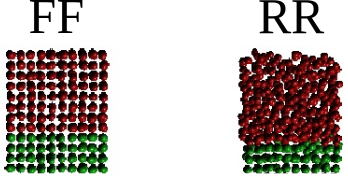
\includegraphics[width=80mm]{rysunki/FFRR.pdf}
\caption{Ilustracja budowy ściany krystalicznej (FF) i amorficznej (RR).}
\label{FFRR}
\label{mapa_stanow}
\end{figure}
%
\section{Szczegóły symulacji}
%
Badany układ składał się z $N=N_A + N_B + N_C =$ 2592 atomów, początkowo ustawionych w bloku o strukturze regularnej ściennie centrowanej. Blok składał się z $[6 \times 6 \times 18]$ czteroatomowych komórek podstawowych. Periodyczne warunki brzegowe zastosowano w płaszczyźnie $xy$. W kierunku $z$ układ był ograniczony fizycznymi ścianami. Liczba cząsteczek w części B wynosiła $N_B = 1440$. Każda ze ścian była zbudowana z 4 warstw. Liczba cząsteczek w każdej ze ścian $N_A = N_C =$ 576. Cząsteczki oddziaływały ze sobą potencjałem Lennarda-Jonesa (z odcięciem $\sigma=2.5$), którego podstawowe parametry odpowiadały oddziaływaniu w Argonie, tzn. $\epsilon / k_B = 120 K$, oraz $\sigma = 0.340$ nm. Studnia potencjału oddziaływania międzycząsteczkowego atomów w ścianach, była dodatkowo skalowana czynnikiem $a_1$ (w większości przypadków $a_1=10$). Skalowanie siły oddziaływania zapewnia stabilność ścian i zapobiega wnikaniu cząsteczek ograniczonej części do wnętrza ścian. Wartości ciśnienia i prędkości ścinania w tej części są wyrażone w jednostkach SI. Temperatura ścian była kontrolowana za pomocą metody skalowania prędkości z korekcją pędu (opisana w sekcji \ref{skal_pr}), była stała i wynosiła $T=120$ K. Równania ruchu całkowane były algorytmem Verleta skaczącej żaby (leap frog) z krokiem czasowym $dt = 0.005$. Symulacje przeprowadzono w ponad 400 punktach $(v_0, P_N)$ utworzonej z 21 wartości zewnętrznego ciśnienia $P_N$, które zmieniało się w zakresie 0-2000 MPa, oraz 21 wartości prędkości ścinania, której wartość zmieniała się w zakresie 0-200~m/s. Czas trwania symulacji w każdym punkcie $(v_0, P_N)$ wynosił 1000 zredukowanych jednostek czasu (co odpowiada 2.5 ns), po wstępnych przebiegach równowagujących, o takim samym czasie trwania. Współczynnik tarcia otrzymano jako średnią po czasie z wyrażenia (\ref{moj_wsp_tarcia}), tzn.~$\langle \mu \rangle = N_W \gamma \langle \Delta v(t) \rangle / P_N S$. Współczynnik tarcia obliczano również jako stosunek średnich sił reakcji ścian w kierunku $x$ i $z$. Obie wartości współczynnika tarcia były takie same w ramach niepewności numerycznej. W tym rozdziale zostaną przedstawione zarówno mapy współczynnika tarcia jak i siły tarcia.
%
%
\section{Stany stacjonarne w układzie ścian krystalicznych~(FF)}
%
W ograniczonej części układu (obszar B) mamy do czynienia z formowaniem się różnych stanów stacjonarnych, w zależności od przyłożonego ciśnienia i prędkości ścinania.
\begin{figure}
\centering
\includegraphics[width=100mm]{rysunki/PRE16_fig7_8.pdf}
\caption{Panel (a) - uzyskana mapa stanów stacjonarnych $(v_0, P_N)$. Na rysunku zaznaczono obszary realizacji poszczególnych stanów za pomocą skrótów L, SK-SL, PS i CL (odpowiednio, stan ciekły - Liquid, stan drgań ciernych - Stick-Slip, stan nieruchomego czopu - Plug-Slip, stan centralnej lokalizacji - Central Localization). Symbol TR oznacza obszar przejściowy, gdzie identyfikacja stanów stacjonarnych była niejednoznaczna. Panel (b) - Mapa współczynnika tarcia $\langle \mu \rangle(v_0, P_N)$ dla układu FF. Skalę współczynnika tarcia zamieszczono po prawej stronie w skali szarości. Granice pomiędzy obserwowanymi stanami stacjonarnymi zostały naniesione w formie przerywanej czerwonej linii. Gwiazdki przedstawiają punkty $(v_0, P_N)$ wykorzystane w badaniach przedstawionych na rysunku \ref{twardosc}.}
\label{mapa_stanow}
\end{figure} 
\linebreak
Niektóre z obserwowanych stanów są znane i obserwowano je wcześniej (np. stan nieruchomego czopu) \cite{DMH1, Gattinoni2013}, ale ich właściwości i obszar tworzenia $(v_0, P_N)$ nie zostały dostatecznie ustalone. W rozprawie znaleziono również nowe typy stanów stacjonarnych, związane przede wszystkim z możliwą orientacją nieruchomego czopu pomiędzy ścianami oraz charakterem cyklicznego topnienia układu w stanie drgań ciernych. 
%
Badania pokazały, że w układzie realizują się cztery jakościowo różne typy stanów stacjonarnych - stan ciekły (Liquid - L), stan centralnej lokalizacji (Central Localization - CL), stan drgań ciernych (Stick-Slip - SK-SL) oraz stan nieruchomego czopu (Plug-Slip - PS). Obszary dobrze określonych zachowań są rozdzielone obszarem przejściowym (Transition Region - TR), w którym jednoznaczna identyfikacja tworzącego się stanu była niemożliwa. \linebreak
Obszary realizacji stanów stacjonarnych $(v_0, P_N)$ zostały przedstawione na rysunku \ref{mapa_stanow}(a). Poszczególne stany identyfikowano w oparciu o profile prędkości $v(z)$, temperatury $T(z)$, gęstości $\rho(z)$ oraz monitorowanie dynamiki cząsteczek. 
%
%
Rysunek \ref{mapa_stanow}(b) przedstawia mapę współczynnika tarcia, gdzie każdemu punktowi $(v_0, P_N)$ przyporządkowano wartość odpowiadającą uśrednionemu współczynnikowi tarcia. Na mapę naniesiono przerywaną czerwoną linię, która ilustruje obszary realizujących się stanów stacjonarnych. Zestawienie obu wykresów ukazuje wyraźną korelację pomiędzy obserwowanymi stanami stacjonarnymi a odpowiadającym współczynnikiem tarcia. Rysunek \ref{mapa_stanow} stanowi główny wynik rozprawy.\\
Poniżej przedstawiono charakterystykę poszczególnych stanów stacjonarnych. 
%
\subsection{Stan ciekły (Liquid)}
Przykładowe realizacje stanu ciekłego (Liquid, L) wraz z odpowiadającymi wartościami ciśnienia i prędkości ścinania zostały przedstawione na rysunku \ref{liquid}. W tym stanie, cząsteczki ograniczonej części, wykazują zachowanie typowe dla cieczy. Cząsteczki mogą dotrzeć do każdego punktu obszaru B, natomiast unormowany i uśredniony (po czasie) profil prędkości $v(z)$ wzdłuż kierunku $z$ jest liniowy (tak jak w klasycznym przepływie Couette, który omówiono w dodatku \ref{dodatekA}), poza obszarem bliskim ścianom. Profil temperatury $T(z)$ jest paraboliczny, natomiast profil gęstości $\rho(z)$ gładki w środkowej części układu, za wyjątkiem oscylacyjnego charakteru w pobliżu ścian. Struktura cieczy przy ścianie jest dobrze znanym i wyjaśnionym efektem \cite{Ladd1977, Cape1982}. Wartości współczynnika tarcia w tym stanie są względnie niskie i nie przekraczają wartości $0.1$ (wartość typowa dla cieczy LJ). Na diagramie stanów stacjonarnych we współrzędnych ($v_0$, $P_N$), \linebreak stan ciekły odpowiada niskim ciśnieniom. Obszar ten można z dobrym przybliżeniem przedstawić prostą zależnością $P_N < 173 + 4.16 v_0$.  
%
\begin{figure}
\centering
\includegraphics[width=160mm]{rysunki/PRE16_fig2.pdf}
\caption{Chwilowe położenia cząsteczek w płaszczyźnie $xz$ dla trzech różnych punktów $(v_0, P_N)$ odpowiadające stanowi ciekłemu (L). Wartości $v_0$ i $P_N$ zostały zamieszczone na wykresie. Ściany ograniczające układ z góry i z dołu oznaczono kolorem czerwonym. Ograniczone cząsteczki oznaczono kolorem  zielonym. Strzałki w ścianach oznaczają kierunek ścinania. Wzdłuż układów zamieszczono profile średniej gęstości $\rho(z)$, prędkości $v(z)$ i temperatury $T(z)$.}
\label{liquid}
\end{figure}
%
%
\subsection{Stan centralnej lokalizacji (Central Localization)}
%
Ten typ stanu stacjonarnego powstaje gdy zewnętrzne ciśnienie przyłożone do układu jest wystarczające aby wywołać uporządkowanie cząsteczek w obszarze B w bezpośrednim sąsiedztwie ścian. Taką sytuację przedstawia rysunek \ref{CL} dla wybranych wartości $(v_0, P_N)$. W porównaniu do stanu ciekłego (L), obserwowany profil prędkości ma znacznie większe nachylenie w centralnej części układu, niż w sytuacji klasycznego przepływu Couette ($2v_0 / h$). Profil temperatury jest paraboliczny wewnątrz centralnej części, gdzie układ jest w stanie ciekłym, natomiast w obszarze stałym ma charakter liniowy (pomiędzy obszarem A/C, a ciekłą częścią układu w centrum). Profil gęstości potwierdza, że~cząsteczki w bezpośrednim sąsiedztwie ścian A i C uległy uporządkowaniu krystalicznemu. W tym stanie współczynnik tarcia jest wyższy niż w sytuacji stanu (L) i mieści się w przedziale wartości $0.1-0.25$. 
%
\begin{figure}
\centering
\includegraphics[width=160mm]{rysunki/PRE16_fig3.pdf}
\caption{Analogiczna ilustracja obserwowanych stanów, tak jak na rysunku \ref{liquid}, ale dla stanu centralnej lokalizacji (CL). }
\label{CL}
\end{figure}
%
\subsection{Stan drgań ciernych (Stick-Slip)}
Przykładowe konfiguracje cząsteczek wraz z odpowiadającymi profilami prędkości, temperatury i gęstości dla SK-SL zostały przedstawione na rysunku \ref{stick-slip}. 
%
\begin{figure}
\centering
\includegraphics[width=160mm]{rysunki/PRE16_fig4.pdf}
\caption{Analogiczna ilustracja obserwowanych stanów, tak jak na rysunku \ref{liquid}, ale dla stanu drgań ciernych (SK-SL).}
\label{stick-slip}
\end{figure}
%
Drgania~cierne są interesującym stanem stacjonarnym, w trakcie którego dochodzi do cyklicznych zmian wartości rejestrowanego współczynnika tarcia. Cykliczna zmiana wartości współczynnika tarcia może być konsekwencją różnych zjawisk, np. następującego po sobie topnienia i krzepnięcia materiału w kontakcie lub wspinania się po sobie współpracujących powierzchni. Wartość współczynnika tarcia zawiera się w zakresie \linebreak $\langle \mu \rangle \simeq 0.25 - 0.5$. To zachowanie obserwowano dla względnie niskich prędkości ścinania w zakresie $0<v_0<30$~m/s oraz w zakresie ciśnień $400< P_N < 800$ MPa. \linebreak Drgania~cierne w skali atomowej obserwuje się od lat 80-tych w szczególności przy wykorzystaniu technik mikroskopii sił atomowych (AFM) oraz za pomocą aparatu sił powierzchniowych (SFA) \cite{Israelachvili1988, Homola1989, McGuiggan1989, Gee1990}. Warto zwrócić uwagę, że profil prędkości $v(z)$ oraz temperatury $T(z)$ mogą być uznane, za odpowiadające stanowi płynnemu. Z kolei profil gęstości $\rho(z)$ ujawnia uporządkowanie translacyjne w układzie. \\
Zgodnie z otrzymanymi wynikami i wykonaną szczegółową analizą zmian konfiguracji cząsteczek, w stanie drgań ciernych układ przechodzi periodyczną w czasie zmianę stanu skupienia - kryształ ulega topnieniu w warstwach. 
%
Rysunek \ref{st-sl-state} przedstawia proces periodycznego topnienia (chwilowe konfiguracje cząsteczek), czasowy przebieg współczynnika tarcia w układzie oraz szerokość układu (obliczaną jako dystans pomiędzy środkami masy ograniczających ścian). 
\begin{figure}
\centering
\includegraphics[width=160mm]{rysunki/PRE16_fig5.pdf}
\caption{Chwilowy współczynnik tarcia rejestrowany w układzie (linia czarna) oraz chwilowa szerokość układu w kierunku $z$ obliczana jako dystans pomiędzy środkami mas ograniczających ścian (linia czerwona). Poszczególne etapy procesu (zatrzymanie/stick i poślizg/slip) oznaczono wraz z odpowiadającym im chwilowym pozycjom cząsteczek.}
\label{st-sl-state}
\end{figure}
Przebiegi $\mu(t)$ oraz $L(t)$ potwierdzają obecność stanu drgań ciernych. Jeden cykl drgań składa się z dwóch części. W pierwszej, układ ulega odkształceniu, a współczynnik tarcia rośnie. Następnie, w pewnej chwili, układ ulega lokalnemu topnieniu, współczynnik tarcia maleje, a układ doznaje skokowego przemieszczenia w~kierunkach ścinania. Za mechanizmem topnienia w warstwach, a nie w całej objętości, przemawia profil gęstości na rysunku \ref{stick-slip}. Gdyby topnienie dotyczyło całego obszaru, profil $\rho(z)$ byłby gładki. Ostre maksima wskazują, że cząsteczki są zlokalizowane w obrębie swoich warstw. Celem upewnienia się co do charakteru topnienia układu, sprawdzono czasowe przebiegi położeń poszczególnych cząsteczek. \\Rysunek \ref{SS-ruch-1-cz} przedstawia zależność współrzędnych $x, y, z$ od czasu dla przypadkowo wybranej cząsteczki z obszaru w którym zachodziły drgania cierne.
%
\begin{figure}[h]
\centering
\includegraphics[width=160mm]{rysunki/SS-ruch-1-cz.pdf}
\caption{Zależność współrzędnych $x,y,z$ przypadkowo wybranej cząsteczki z obszaru w którym zachodziły drgania cierne. Rysunek ujawnia, że w kolejnych cyklach cząsteczka miała swobodę zmiany położenia w kierunkach $x,y$, ale wciąż średnio pozostawała w tej samej warstwie o ustalonej pozycji $z$. Po prawej stronie zamieszczono chwilowe położenia cząsteczek centralnej warstwy układu w fazie "stick" i fazie "slip".}
\label{SS-ruch-1-cz}
\end{figure}
%
W trakcie drgań ciernych, cząsteczka zmienia swoją pozycję w kierunkach $x$ i $y$, ale pozostaje średnio nieruchoma w kierunku $z$. Sugeruje to mechanizm topnienia układu w warstwach.
%
%
%
%
%
%
\subsection{Stan nieruchomego czopu (Plug-Slip)}
Obszar stanów stacjonarnych na mapie $(v_0, P_N)$ w zakresie $v_0<50$~m/s \linebreak oraz~$P_N>700$~MPa wiąże się z obecnością krystalicznego, nieruchomego czopu \linebreak wewnątrz obszaru ograniczonego. Obszar ten ujawnia najbardziej zróżnicowane zachowania tribologiczne (w porównaniu do wcześniej omówionych stanów). Przykładowe realizacje stanu PS zostały przedstawione na rysunku \ref{ps-state}. Najczęściej pojawiającą się realizacją stanu PS jest nieruchomy czop rozdzielający ruchome ściany. Orientacja oraz struktura czopu może różnić się od orientacji i struktury ścian układu.
%
\begin{figure}[h]
\centering
\includegraphics[width=160mm]{rysunki/PRE16_fig6.pdf}
\caption{Ilustracja stanu nieruchomego czopu (Plug-Slip, PS) dla wybranych punktów $(v_0, P_N)$. Opis zgodny z rysunkami \ref{liquid} i \ref{stick-slip}. Nieruchomy czop został zaznaczony niebieskim prostokątem. Dodatkowo zaznaczono interfejsy czopu i ruchomej ściany literami "D" dla kontaktu suchego oraz "W" dla kontaktu zwilżonego.}
\label{ps-state}
\end{figure}
%
%
\\
Zdefiniowano dwa rodzaje lokalizacji ścinania. Jeżeli profil prędkości $v(z)$ w interfejsie pomiędzy czopem i ścianą ujawnia gwałtowną zmianę wartości na przestrzeni około jednej warstwy atomowej (tak jak na rysunku \ref{ps-state}(c)), można uznać, że kontakt jest suchy (\textit{ang.} dry) i będziemy oznaczać go literą "D". Z kolei, jeżeli zmiana wartości profilu prędkości zachodzi na przestrzeni co najmniej trzech warstw atomowych (tak jak na rysunku \ref{ps-state}(a) i (b)) można uznać, że interfejs jest zwilżony (\textit{ang.} wet) i będziemy oznaczać go literą "W". W~rzeczywistości interfejs może zmieniać się w czasie, co dodatkowo utrudnia identyfikację i podział na interfejs suchy i zwilżony, ponieważ mogą one występować po~sobie w czasie. Szczególnym przypadkiem stanu PS jest sytuacja, w której czop łączy się ze ścianą i dalej jest przez nią prowadzony. Taki stan stacjonarny można zidentyfikować m.~in.~dzięki analizie profili prędkości. Dla przykładu, na panelu (a) rysunku \ref{ps-state}, który odpowiada warunkom $v_0=10$~m/s, $P_N=1100$ MPa, można zauważyć, że czop jest przyczepiony i prowadzony przez górną ścianę, ponieważ (co wynika z profilu prędkości) czop i ściana mają takie same prędkości.

Tarcie jako ogół mechanizmów związanych z rozpraszaniem uporządkowanego pędu cząsteczek, zależy między innymi od właściwości współpracujących powierzchni atomowych. Rysunek \ref{ps-state} (c) pokazuje interesującą sytuację, w której zaobserwowano czop otoczony dwoma suchymi kontaktami. Profil prędkości $v(z)$ ujawnia gwałtowną zmianę. Wielokrotne testy i obserwacje mniejszych części układu każą sądzić, że w tej sytuacji topografia powierzchni czopu i ścian jest różna. 
%
\begin{figure}[h]
\centering
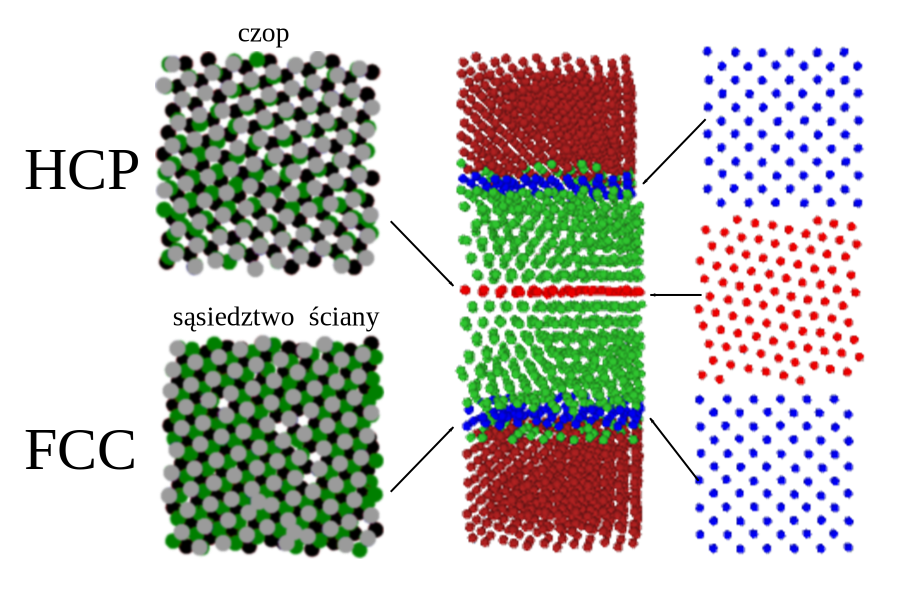
\includegraphics[width=160mm]{rysunki/PS-orientacja-czopu.pdf}
\caption{Chwilowe położenia cząsteczek układu w stanie PS oraz w sytuacji kontaktów suchych (interfejsy typu "D"). Po prawej stronie zamieszczono przekroje układu w warstwach odpowiadających sąsiedztwu ruchomych ścian (warstwy niebieskie) oraz w warstwie odpowiadającej środkowi nieruchomego czopu. Widać, że struktury powierzchni przekrojów są różne. Po lewej stronie przedstawiono warstwy układu (kolor zielony) otoczone sąsiadującą warstwą dolną (kolor czarny) i górną (kolor szary). Ułożenie kolejnych warstw wskazuje na obecność struktury HCP w czopie.}
\label{PS-orientacja-czopu}
\end{figure}
Identyfikacja struktury krystalicznej \linebreak oraz topografii czopu nie jest jednoznaczna. Rysunek \ref{PS-orientacja-czopu} przedstawia chwilowe położenia cząsteczek w układzie, widok przekroju układu w warstwach odpowiadających sąsiedztwu ścian (zaznaczone na niebiesko) oraz środkowej części nieruchomego czopu. Rysunek \ref{PS-orientacja-czopu} potwierdza, że geometrie powierzchni czopu i ruchomych ścian są różne. Dodatkowe testy struktury krystalicznej czopu i ścian oraz analiza diagramu fazowego układu cząsteczek Lennarda-Jonesa pozwalają wysunąć wniosek, że w rozważanym przypadku nieruchomy czop miał strukturę HCP. Za realizacją struktury HCP przemawia m. in. uporządkowanie kolejnych warstw atomowych w czopie. Na rysunku \ref{PS-orientacja-czopu} przedstawiono chwilowe położenia cząsteczek w warstwie czopu i w warstwie bliskiej ściany układu (kolor zielony) wraz ze spodnią i wierzchnią warstwą (oznaczone odpowiednio kolorami czarnym i szarym). Uporządkowanie warstw wskazuje na obecność struktury FCC w ścianach oraz HCP w czopie. Ruch ścian po powierzchni czopu odbywa się wzdłuż kierunków łatwego poślizgu. Współczynnik tarcia przyjmował ekstremalnie niskie wartości, niemal równe zeru. Pokrywa się to z ogólną wiedzą dotyczącą zjawiska nadśliskości, które zachodzi, kiedy przesuwane są po sobie dwie suche powierzchnie atomowe o niewspółmiernych stałych sieciowych. 
%
\section{Mapa siły tarcia w układzie (FF)}
%
%
Na podstawie rysunku \ref{mapa_stanow} wyznaczono mapę siły tarcia.
%
Rysunek \ref{mapa3DFF} przedstawia trójwymiarową mapę tarcia dla układu ograniczonego ścianami krystalicznymi.
Zauważalną cechą mapy tarcia jest nietrywialna natura tribologiczna stanu PS. 
%
\begin{figure}[h]
\centering
\includegraphics[width=120mm]{rysunki/PRE16_fig13.pdf}
\caption{Trójwymiarowa mapa siły tarcia $\langle F_f \rangle(v_0, P_N)$ dla układu FF. Czerwona przerywana linia w lewym górnym rogu wskazuje granicę nieregularności w zachowaniu siły tarcia. Czerwona, niebieska i czarna linia reprezentuje wybrane zachowania dla prędkości ścinania $v_0$ równej 20, 100 i 180~m/s.}
\label{mapa3DFF}
\end{figure}
%
%
Wartość siły tarcia w tym stanie zmienia się od umiarkowanych wartości (podobnych jak w stanie CL) do ekstremalnie małych, bliskich zeru (w przypadku czopu z suchym interfejsem). W układach makroskopowych, siła tarcia jest zwykle proporcjonalna do przyłożonego obciążenia (I prawo Amontona). W badanym układzie widać, że I prawo Amontona jest w przybliżeniu spełnione, poza obszarem odpowiadającym stanowi PS. Rysunek \ref{mapa3DFF} ilustruje jakościową różnicę zależności tarcia od zewnętrznego ciśnienia w obszarze PS (obszar zaznaczony czerwoną linią przerywaną). Na mapie naniesiono również linie odpowiadające jej przekrojom. Przekroje mapy siły tarcia potwierdzają zgodność zachowania układu z I prawem Amontona dla prędkości ścinania powyżej $75$~m/s (linia granatowa i czarna) oraz anomalne zachowanie dla mniejszych prędkości ścinania (linia czerwona). Na podstawie otrzymanych wyników można powiedzieć, że w stanie PS siła tarcia może maleć wraz ze wzrostem obciążenia, co jest niezwykłym zachowaniem. Współczynnik tarcia można definiować jako pochodną zależności siły tarcia od siły nacisku $\mu' = {dF_f}/{dF_N}$ (różniczkowy współczynnik tarcia, RWT). \\We fragmentach stanu PS tak zdefiniowany współczynnik tarcia ma znak ujemny. Zjawisko ujemnego RWT zostało niedawno zaobserwowane eksperymentalnie w układzie modyfikowanej chemicznie powierzchni grafitu badanej mikroskopem sił atomowych w trybie mikroskopii sił tarcia~\cite{Deng2012}. W przypadku wykonanych symulacji efekt ujemnego różniczkowego współczynnika tarcia zaobserwowano w relatywnie prostym układzie. Podstawowym procesem odpowiedzialnym za negatywną wartość pochodnej zależności $F_f(F_N)$ jest zmiana struktury czopu indukowana zmianą zewnętrznych warunków $(v_0, P_N)$. Negatywna wartość różniczkowego współczynnika tarcia jest zaskakującym wynikiem i może mieć praktyczne znaczenie w wyznaczaniu optymalnych ścieżek $(v_0, P_N)$ procesów technologicznych.\\
Mapa tarcia wskazuje również, że w układzie nie jest spełnione prawo Coulomba, chociaż można wyróżnić fragmenty w obszarach L i CL, gdzie ta zależność jest nieznaczna lub ma charakter liniowy. Powyższa obserwacja pokrywa się z wynikami innych badań tarcia w skali molekularnej \cite{Braun2006, Socoliuc2004}.   
%
%\clearpage
\section{Histereza w układzie (FF)}
%
%
W układzie ograniczonym ścianami FF zaobserwowano wpływ historii prowadzenia układu do danego punktu $(v_0, P_N)$ na otrzymywane wyniki. Obliczenia wykonano przy stałych wartościach ciśnienia $P_N$, zwiększając stopniowo prędkość ścinania od $v_0=0$ do $v_0=200$~m/s, z krokiem $\delta v_0 = 0.15$~m/s, co każde 10 kroków symulacji. Każda wartość $v_0$ została otrzymana z dokładnością do prędkości ruchu fluktuacji termicznych. Uzyskana mapa współczynnika tarcia jest przedstawiona na rysunku \ref{mapa_historia}. 
\begin{figure}[h]
\centering
\includegraphics[width=100mm]{rysunki/PRE16_fig11.pdf}
\caption{Mapa współczynnika tarcia dla układu (FF), analogiczna do mapy przedstawionej na rysunku \ref{mapa_stanow}(b), ale uzyskana przy wzroście prędkości ścinania od małych wartości, bliskich zeru, przy stałym, zadanym ciśnieniu zewnętrznym $P_N$. Niebieski prostokąt naniesiony przerywaną linią wskazuje przykładowy obszar, w którym uzyskana wartość współczynnika tarcia zależy od historii prowadzenia układu. Uzyskany wynik wyjaśnia rysunek \ref{historia_stany}.}
\label{mapa_historia}
\end{figure}
Mapa współczynnika tarcia uzyskana w trakcie analogicznego procesu, ale przy stopniowym zmniejszaniu prędkości od wartości $v_0=200$~m/s do $v_0=0$~m/s, przy zadanych wartościach $P_N$ jest~jakościowo podobna do mapy przedstawionej na rysunku \ref{mapa_stanow}. Wpływ historii układu na otrzymywane wyniki jest zaniedbywalny w obszarach odpowiadających stanom L, CL oraz SK-SL, natomiast może mieć znaczny wpływ na wyniki otrzymywane w obszarze PS.
%
Rysunek \ref{mapa_historia} pokazuje, że zwiększanie prędkości ścinania układu z punktu $(v_0, P_N)$ w obszarze PS, w kierunku obszaru CL, (np. dla $P_N \approx 1500$ MPa oraz prędkości ścinania w zakresie pomiędzy $25$ i $75$~m/s), \\daje w wyniku inne zachowanie tribologiczne niż te przedstawione na rysunku \ref{mapa_stanow}(b). 
Prostokątny obszar zaznaczony niebieską, przerywaną linią, odpowiada nowemu typowi zachowania, które wiąże się z bardzo niskim współczynnikiem tarcia, może być utrwalone i przeniesione daleko w obszar stanu CL. Chwilowe położenia atomów odpowiadające omawianej sytuacji (ciśnienie $P_N=1500$ MPa, $v_0 \in (25, 75)$~m/s), przedstawiono na rysunku \ref{historia_stany}. 
\begin{figure}[h]
\centering
\includegraphics[width=135mm]{rysunki/PRE16_fig12.pdf}
\caption{Chwilowe położenia cząsteczek dla ciśnienia $P_N=1500$ MPa. Podkreślony obszar (niebieski prostokąt) odpowiada ramce na rysunku \ref{mapa_historia}. Górny wiersz ramki odpowiada zwiększaniu prędkości ścinania, natomiast dolny zmniejszaniu prędkości ścinania.}
\label{historia_stany}
\end{figure}
Górny wiersz ramki odpowiada zwiększaniu prędkości ścinania, natomiast dolny - zmniejszaniu. W trakcie zwiększania prędkości ścinania, można zaobserwować, że w stanie odpowiadającym wartości $v_0 \approx 60$~m/s, nieruchomy czop w ograniczonej części ulega zmianie struktury, która w efekcie ułatwia proces poślizgu i jest bardzo stabilna - zwiększanie prędkości nie wywołuje jej zniszczenia. Dokładna analiza interfejsu pomiędzy ruchomymi ścianami a powstałym czopem wskazuje, że współpracujące powierzchnie są różne i prawdopodobnie niewspółmierne \cite{SpringerHandbook}. Obserwowana sytuacja może odpowiadać zjawisku "nadśliskości", w którym energia drgań sieci krystalicznej układu ułatwia przemieszczanie się po sobie współpracujących powierzchni i skutkuje niemal zerowym współczynnikiem tarcia. Uzyskane wyniki wskazują, że w badanym układzie mamy do czynienia z takim zjawiskiem. Dodatkowo, pokazano, że stan odpowiadający temu zjawisku, jest wyjątkowo trwały i odporny na zmiany prędkości ścinania. Z kolei w trakcie obniżania prędkości ścinania, efekt "nadśliskości" nie wystąpił. Wskazuje to, że układ może być wrażliwy na historię prowadzenia procesu, przechodząc od stanu PS. Jeżeli w stanie PS układ przeorganizuje orientację i strukturę czopu, do takiej, która obniży współczynnik tarcia, może ulec "utrwaleniu" w danym stanie i przeniesieniu w~jakościowo niezmienionej formie w obszar $(v_0, P_N)$ właściwy stanowi CL. Zaobserwowany efekt może mieć szczególne znaczenie z punktu widzenia zastosowań. W praktyce tribologicznej często pożądanym jest, aby kontrolować tarcie w trakcie prowadzenia procesu. Zależność współczynnika tarcia od historii, może pozwolić na znalezienie optymalnych ścieżek prowadzenia układu, który zapewni odpowiedni (najmniejszy bądź największy) współczynnik tarcia. 
%
%
%
%
%
%
%
\section{Wpływ postaci potencjału Lennarda-Jonesa na współczynnik tarcia}
\label{a1a2}
%
%
Ostatnim problemem, jaki został przebadany w układzie FF był wpływ oddziaływania między cząsteczkami w ścianach ($u_{AA}$, $u_{CC}$) oraz oddziaływania między ścianami a układem cząsteczek ($u_{AB}$, $u_{BC}$) na współczynnik tarcia.
\\
Potencjał LJ opisany równaniem (\ref{LJPOT}) był modyfikowany wartością czynników $a_1$ i $a_2$. 
Czynnik $a_1$ odpowiada sile wzajemnego oddziaływania cząsteczek. Dla par cząsteczek poza obszarem ścian, wartość $a_1$ była równa jedności. Dla par cząsteczek w ścianach wartość $a_1$ zmieniano w zakresie od $a_1=2.5$ do $a_1=10$. Wzrost wartości $a_1$ między cząsteczkami ścian zmniejsza prawdopodobieństwo wniknięcia cząsteczek ograniczonej części do obszaru ścian. Można powiedzieć, że w przypadku oddziaływania między cząsteczkami ścian $u_{AA}$, $u_{CC}$, wartość $a_1$ wiąże się z twardością ścian. Ważnym pytaniem jest czy oddziaływanie $u_{AA}$, $u_{CC}$ wpływa na własności fizyczne układu, w szczególności w jakim stopniu wpływa na wartość współczynnika tarcia $\langle \mu \rangle$. Aby odpowiedzieć na tak postawiony problem, wykonano serię symulacji dla układów w ustalonych warunkach $(v_0, P_N)$. Punkty $(v_0, P_N)$ w których przeprowadzono testy, zostały zaznaczone na rysunku \ref{mapa_stanow}(b) w postaci gwiazdek. Uzyskane wyniki (dla ciśnienia $P_N=1500$~MPa oraz prędkości $v_0=50,~60,~80,~100$~m/s) przedstawia rysunek \ref{twardosc} (a). 
%
\begin{figure}[h]
\centering
\includegraphics[width=160mm]{rysunki/PRE16_fig9.pdf}
\caption{Zależność współczynnika tarcia od dwóch parametrów potencjału Lennarda-Jonesa, $a_1$ i $a_2$ (równanie (\ref{LJPOT})). Obliczenia wykonano dla (a) ustalonej wartości $a_2=1$ oraz różnych wartości $a_1$, (b) ustalonej wartości $a_1=2.5$ oraz różnych wartości $a_2$ wykorzystanych w obliczaniu oddziaływania cząsteczek w układzie. Wartość $P_N$ oraz $v_0$ odpowiada przejściu od stanu CL do L przy ciśnieniu $P_N=500$ MPa. Kolejne kolory linii i znaczniki wskazują kolejne prędkości ścinania. Punkty w których wykonano wymienione testy zostały wskazane na mapie współczynnika tarcia, przedstawionej na rysunku \ref{mapa_stanow}(b) za pomocą gwiazdek.}
\label{twardosc}
\end{figure}
\\
Wynik pokazuje, że wzrost wartości $a_1$ powoduje spadek wartości współczynnika tarcia $\langle \mu \rangle$. Taki sam trend uzyskano dla wszystkich testowanych prędkości ścinania. Obserwowany spadek jest liniowy, natomiast jego wartość jest znacząca, zazwyczaj przekracza $2\%$ na zmianę $a_1$ o jedność. 

W tych samych punktach $(v_0, P_N)$ przebadano związek między współczynnikiem tarcia $\langle \mu \rangle$, a wartością $a_2$. Parametr $a_2$ był zmieniany tylko dla oddziaływań cząsteczek w~ograniczonej części z cząsteczkami ścian, a więc modyfikował oddziaływania $u_{AB}$, $u_{BC}$. W pozostałych przypadkach był równy 1. Czynnik $a_2$ nazywa się często parametrem zwilżania, ponieważ za jego pomocą można kontrolować przyleganie cząsteczek ograniczonej części do ścian układu. Wyniki wykonanych testów przedstawiono na rysunku \ref{twardosc} (b). Na jego podstawie, można powiedzieć, że wraz ze wzrostem wartości czynnika $a_2$ współczynnik tarcia $\langle \mu \rangle$ rośnie. Uzyskany trend jest liniowy, natomiast jego wartość nie przekracza $1\%$ na zmianę $a_2$ o jedność. Przedstawione wyniki wskazują, że wpływ wartości $a_1$ oraz $a_2$ na współczynnik tarcia nie jest zaniedbywalny. Porównując wyniki różnych symulacji, należy uwzględnić przedstawioną zależność.  

Czynniki $a_1$ i $a_2$ wpływają na statystykę zderzeń pomiędzy ograniczonymi cząsteczkami a ścianami układu. Zjawisko tarcia polega na rozpraszaniu energii kinetycznej ruchu postępowego w układzie na energię ruchu chaotycznego (tym samym produkując ciepło). W~związku z~tym, można spodziewać się, że zmiana dynamiki zderzeń będzie mieć wpływ na współczynnik tarcia w układzie, co potwierdza rysunek \ref{twardosc}. Ta zależność jest w szczególności widoczna w wysokich ciśnieniach (przykładowo w przedziale od $P_N = 500$ do $1000$ MPa) gdzie sprzężenie pomiędzy ograniczoną częścią a ścianami jest silne. Związku pomiędzy współczynnikiem tarcia a czynnikami $a_1$, $a_2$ nie zauważono w obszarze niskich ciśnień (np. $P_N=100$ MPa), odpowiadających stanowi ciekłemu, gdzie wpływ wartości $a_1$, $a_2$ jest rozproszony w całej objętości zajmowanej przez ograniczony płyn. Gdy wartość $a_1$ rośnie (a wraz z nią twardość ścian), zmniejsza się rozpraszanie energii kinetycznej cząsteczek obszaru B przez oddziaływanie ze ścianami - wówczas współczynnik tarcia maleje. Z kolei gdy wartość parametru zwilżania $a_2$ rośnie, przyciąganie, bądź adhezja cząsteczek ograniczonej części do ścian układu rośnie, co wywołuje wzrost współczynnika tarcia. Ciekawym faktem jest również charakter znalezionej zależności pomiędzy $a_1$, $a_2$ i $\langle \mu \rangle$, która zgodnie z wynikami przedstawionymi na rysunku \ref{twardosc} jest liniowa. Uzyskane wyniki wskazują, że arbitralny dobór stałych oddziaływania może mieć wpływ na wartość współczynnika tarcia w układzie. Otrzymane zależności wskazują, że wiązanie atomów ścian za pomocą sprężyn o arbitralnych wartościach $k$ ma wpływ na otrzymywane wyniki współczynnika tarcia.
%
\section{Mapa stanów stacjonarnych i współczynnika tarcia w układzie ścian amorficznych (RR)}
%
Wyniki przedstawione i omówione w poprzednich sekcjach, były prowadzone w układach ograniczonych ścianami krystalicznymi o strukturze regularnej powierzchniowo centrowanej. W tej części zostaną przedstawione wyniki dla układu o ścianach amorficznych.
Można się spodziewać, że struktura oraz chropowatość ścian, może mieć wpływ na właściwości tribologiczne układu \cite{Jab2006, Priez2007, sofos2009}. Związek między chropowatością ścian a tarciem, może mieć szczególne znaczenie z punktu widzenia zastosowań. 
%
%\cite{SpringerHandbook, Jab2006, Priez2007, sofos2009}. 
%
Chropowatość może wzmagać bądź zmniejszać przepływ i drogę poślizgu w zależności od właściwości ścian i warstwy smarującej (np. hydrofilowość i hydrofobowość oddziaływania). Celem tej sekcji jest określenie jakościowego wpływu chropowatości ścian na tworzące się struktury stacjonarne oraz tribologiczny diagram stanów stacjonarnych $(v_0, P_N)$. Rozważana będzie chropowatość o niskiej amplitudzie i periodyczności rzędu rozmiarów molekuł płynu.   
%
%
Amorficzne powierzchnie ścian uzyskano poprzez stopienie, a następnie gwałtowne ochłodzenie całego układu. Tak przygotowana struktura stanowiła punkt wyjścia do uzyskania kolejnych stanów $(v_0, P_N)$. Procedura prowadzenia układu do zadanej wartości prędkości ścinania i ciśnienia była identyczna jak w sekcji dotyczącej układu FF. Każdą wartość ciśnienia i prędkości ścinania otrzymano rozpoczynając obliczenia z tego samego punktu $(v_0, P_N)$, a następnie stopniowo zwiększając $P_N$ i $v_0$ do zadanej wartości o niewielkie przyrosty rzędu $\delta P=42$ Pa oraz $\delta v=0.15$~m/s co 10 kroków symulacji. Dokładne wartości zmiany ciśnienia i prędkości były przypadkowe celem uniknięcia problemów związanych z histerezą pomiędzy sąsiadującymi stanami.\\
%
\begin{figure}[h]
\centering
\includegraphics[width=100mm]{rysunki/stany_wsp_t.pdf}
\caption{Panel (a) - uzyskana mapa stanów stacjonarnych w przestrzeni $(v_0, P_N)$ dla układu (RR). Na rysunku zaznaczono obszary stabilności poszczególnych stanów za pomocą skrótów L, PS, i AM (stan ciekły - Liquid, stan nieruchomego czopu - Plug-Slip, głównie stan asymetrycznego topnienia - Asymmetric Melting). Obszar "Głównie AM" oznacza mieszaninę stanów AM (asymetrycznego topnienia), PS oraz innych, nieuporządkowanych struktur, w oparciu o analizę uśrednionych po czasie profili $\rho(z), v(z), T(z)$ oraz chwilowych położeń cząsteczek. Naniesiona siatka wskazuje przebadane punkty $(v_0, P_N)$. Panel (b) - mapa współczynnika tarcia $\langle \mu \rangle(v_0, P_N)$ dla układu (RR). Skalę współczynnika tarcia zamieszczono po prawej stronie w formie paska w skali szarości. Granice pomiędzy obserwowanymi stanami stacjonarnymi zostały naniesione w formie przerywanej czerwonej linii.}
\label{mapa_stanow_RR}
\end{figure}
\clearpage
Początkowa struktura całego układu  przedstawionego na rysunku \ref{szczelina} była amorficzna. Amorficzność i asymetria układu ma duży wpływ na rodzaj i naturę tworzących się stanów stacjonarnych. Oddziaływanie pomiędzy atomami ścian było stosunkowo duże, dzięki czemu nie obserwowano znaczącego mieszania się bądź wnikania w siebie cząsteczek z sąsiadujących obszarów układu. Struktura ścian (w szczególności jej chropowatość) mogła ulegać lokalnym zmianom pod wpływem zewnętrznego ciśnienia i ścinania. Nie~miało~to~jednak wpływu na obserwowane średnie, w tym mapy stanów stacjonarnych i tarcia.
\\
Rysunek \ref{mapa_stanow_RR} przedstawia mapę $(v_0, P_N)$ stanów stacjonarnych uzyskaną dla układu ograniczonego ścianami amorficznymi (układ RR). 
%
%
\noindent
Uzyskana mapa jest analogiem rysunku \ref{mapa_stanow} uzyskanego dla układu FF. Poszczególne stany stacjonarne były identyfikowane w oparciu o profile gęstości, prędkości, temperatury, współczynnik tarcia oraz chwilowe położenia cząsteczek, podobnie jak w części poświęconej wynikom uzyskanym w układzie FF. Rysunek \ref{mapa_stanow_RR} pokazuje, że wprowadzenie chropowatości w ścianach ma znaczący wpływ na postać mapy stanów stacjonarnych. Można zauważyć, że w porównaniu do mapy układu FF (rysunek \ref{mapa_stanow}(a)), stan L i częściowo stan PS występują w podobnych obszarach mapy. W pozostałych częściach mapy, różnice są znaczne. Nie zaobserwowano obecności stanu SK-SL jak również stanu CL. W układzie zaobserwowano realizację nowego stanu, który polega na asymetrycznym topnieniu ograniczonej części przy jednej ze ścian. Zaobserwowany stan zostanie szczegółowo omówiony poniżej.
%
%
\begin{figure}[h]
\centering
\includegraphics[width=60mm]{rysunki/PRE16_fig15.pdf}
\caption{Chwilowe położenia cząsteczek w płaszczyźnie $xz$ dla wartości $(v_0, P_N)$ odpowiadającej stanowi asymetrycznego topnienia (AM). Wartości zewnętrznego ciśnienia i prędkości ścinania wynoszą odpowiednio $700$ MPa i $70$~m/s. Amorficzne ściany ograniczające układ z góry i z dołu oznaczono kolorem czerwonym. Ograniczony układ cząsteczek oznaczono kolorem zielonym. Strzałki w ścianach oznaczają kierunek ścinania. Wzdłuż układów zamieszczono profile czasowej średniej gęstości $\rho(z)$, prędkości $v(z)$ i temperatury $T(z)$}
\label{AM}
\end{figure}
\noindent
\\
\\
\textbf{Stan asymetrycznego topnienia (Assymetric Melting)} - przykładową realizację tej struktury przedstawia rysunek \ref{AM}. 
Asymetryczne topnienie to stan, w którym układ z jednej strony jest ciągnięty przez ograniczającą ścianę, natomiast poślizg i topienie obszaru interfejsu pojawia się tylko przy jednej ze ścian. Cząsteczki ograniczonej części wypełniają nierówności ścian, tworząc zdefektowana strukturę krystaliczną, która może zostać nadbudowana kolejnymi warstwami. Ze względu na przypadkowość wytwarzanych chropowatości, wytrzymałość układu na ścinanie przy ścianach jest różna z jednej i~z~drugiej strony. W związku z tym, po przyłożeniu obciążenia ścinającego, układ ulega pęknięciu i częściowemu stopieniu z jednej strony. 
\begin{figure}[t]
\centering
\includegraphics[width=120mm]{rysunki/sila_t_RR.pdf}
\caption{Trójwymiarowa mapa siły tarcia $\langle F_f \rangle(v_0, P_N)$ dla układu (RR). Czerwona przerywana linia wskazuje granicę nieregularności w zachowaniu siły tarcia. Czerwona, niebieska i czarna linia reprezentuje wybrane zachowania dla prędkości ścinania $v_0$ równej 20, 100 i 180~m/s.}
\label{sila_tarcia_RR}
\end{figure}
Profil $v(z)$ pokazuje, że poślizg ma miejsce tylko przy jednej ze ścian, przy drugiej z kolei można zauważyć zbudowaną zdefektowaną strukturę krystaliczną (w oparciu o profil gęstości oraz chwilowe konfiguracje cząsteczek). Można powiedzieć, że w stanie AM obecny jest tylko jeden interfejs między współpracującymi obszarami. Na mapie stanów stacjonarnych stan AM miesza się ze stanem PS i stanami których nie można jednoznaczne przypisać do żadnej z ustalonych kategorii. Lokalizacja granic między stanami w tym obszarze nie jest jednoznaczna. Struktura układu ostatecznie zależy od przypadkowego procesu związanego z początkową organizacją cząsteczek w ograniczonej części w pobliżu ścian.\\
Rysunek \ref{sila_tarcia_RR} przedstawia trójwymiarową mapę średniej siły tarcia uzyskaną dla układu RR w zależności od przyłożonego ciśnienia i prędkości ścinania.
%
%
Rysunek odpowiada mapie przedstawionej dla układu FF na rysunku \ref{mapa3DFF}. Uzyskana mapa jest zdecydowanie bardziej gładka. Nie posiada obszarów o ekstremalnie wysokim lub niskim współczynniku i sile tarcia, w przeciwieństwie do wyników układu FF przedstawionych na~rysunkach \ref{mapa_stanow} i \ref{mapa3DFF}. W obszarach odpowiadających stanom L i PS obserwowane właściwości są podobne jak w układzie FF. Pierwsze prawo Amontona jest tylko częściowo spełnione w obszarze L. W częściach Głownie-AM i PS widać anomalne zachowanie tribologiczne, polegające na tym, że wzrost obciążenia może wiązać się z obniżeniem wartości siły (bądź współczynnika) tarcia. Podobne wyniki obserwowano dla stanu PS w układzie FF. 
\\
\\
\\
Rysunek \ref{sila_tarcia_RR} przedstawia przykłady zależności $\langle F_f \rangle(F_N)$ dla trzech różnych wartości $v_0$, gdzie prawo Amontona nie wszędzie jest spełnione. Przerywana czerwona linia rozdziela obszar nieregularności w zachowaniu siły tarcia.
%
\chapter{Podsumowanie i wnioski}
W rozprawie doktorskiej zaproponowano metodę modelowania układów oddziałujących cząsteczek w geometrii szczeliny oraz zbadano związek pomiędzy mikroskopowym tarciem a realizującymi się stanami stacjonarnymi, w warunkach kontrolowanego ciśnienia, ścinania i temperatury. 

W części metodologicznej rozprawy omówione zostały zastosowane równania ruchu, warunki budowy ograniczających ścian, schemat kontroli temperatury, ciśnienia i ścinania. Omówiono wpływ stosowania "sprężyn" do lokalizacji cząsteczek ścian. Badane układy ograniczano fizycznymi ścianami, 
których atomy oddziaływały wyłącznie siłami dwucząsteczkowymi. Wprowadzono schematy kontroli temperatury oparte na skalowaniu prędkości i termostacie Nos\'{e}go-Hoovera, które zachowują całkowity pęd w układzie mikroszczeliny. Omówiono problem obliczania ciśnienia w geometrii szczeliny i przedstawiono trudności związane z obliczaniem kinetycznej części ciśnienia w metodzie płaszczyzn. Przeanalizowano barostaty globalne i zaproponowano barostat mikroskopowy. Wprowadzono schemat ścinania układu oparty na sile działającej na cząsteczki ścian, proporcjonalnej do różnicy pomiędzy względną prędkością ścian, a zadaną prędkością ścinania. Zastosowanie względnych prędkości jest spójne z modelem Petravic, natomiast fizyczną interpretację stałej $\gamma$ uzyskano, wykorzystując jednowymiarowy model Prandtla. Na podstawie wprowadzonych równań ruchu sformułowano nowe wyrażenie na współczynnik tarcia w układzie.

Korzystając z wprowadzonych równań ruchu wykonano program i symulacje NEMD, za pomocą których zbadano generyczny model mikroszczeliny w warunkach $(T, v, P)$. Właściwości fizyczne układu zostały przebadane \begin{samepage} w ponad 400 punktach $(v_0, P_N)$ \end{samepage}. Stany stacjonarne identyfikowano w oparciu o profile prędkości $v(z)$, temperatury $T(z)$, gęstości $\rho(z)$, współczynnik tarcia $\langle \mu \rangle$ oraz chwilowe konfiguracje cząsteczek. Badano układy ograniczone ścianami krystalicznymi (FF) oraz amorficznymi (RR). 

Zestawienie szczegółowych map stanów stacjonarnych z mapami współczynnika i siły tarcia dla układu cząsteczek w geometrii szczeliny w warunkach $(T, v, P)$, ograniczonych ścianami krystalicznymi i amorficznymi stanowi oryginalny wkład do współczesnej wiedzy na temat tarcia.  
Pokazano związek pomiędzy mapą stanów stacjonarnych a mapą współczynnika tarcia. Ponieważ część stanów stacjonarnych wykazuje charakterystyczne wartości współczynnika tarcia może być on indykatorem tworzenia się tych stanów. 
Otrzymane mapy współczynnika i siły tarcia potwierdzają istnienie ścieżek optymalnego tarcia w~procesach opartych na kontroli ciśnienia i prędkości ścinania. Potwierdzają również istnienie obszarów $(v_0, P_N)$, w których klasyczne prawa tarcia mogą być w przybliżeniu spełnione.

W układzie FF zaobserwowano stan drgań ciernych (SK-SL) oraz pokazano, że polega on na cyklicznym topnieniu i krystalizacji układu w warstwach, a~nie w~całej objętości układu, co stanowi nową interpretację mechanizmu tego efektu. W stanie nieruchomego czopu (PS) zauważono, że czop może przyjąć orientację sprzyjającą poślizgowi, w której współczynnik tarcia jest bliski zeru. Pokazano, że niski współczynnik tarcia wiąże się z odmienną topografią powierzchni czopu i ruchomych ścian. Zaobserwowano zależność powstających stanów stacjonarnych w układzie od warunków $(v, P)$ w których układ znajdował się wcześniej. Nieruchomy czop rozdzielający ruchome ściany, o orientacji ułatwiającej poślizg, wpływa na realizację kolejnych stanów na drodze zwiększania prędkości. Badania pokazały, że czop może pozostać stabilny, mimo wzrostu prędkości do wartości $(v_0, P_N)$ odpowiadających stanowi centralnej lokalizacji. 

Badania układu RR ujawniły znaczący wpływ chropowatości na właściwości tribologiczne układu (m. in. na mapy stanów stacjonarnych i współczynnika tarcia). W układzie RR nie zauważono realizacji stanów drgań ciernych i centralnej lokalizacji. Wskazuje to, że stany SK-SL oraz CL wymagają ograniczenia układu za pomocą ścian krystalicznych. W układzie RR obserwowano natomiast nowy typ uporządkowania cząsteczek - stan asymetrycznego topnienia. Polega on na jednostronnym topnieniu obszaru kontaktu ograniczonej części ze ścianą oraz wykazuje asymetrię profilu prędkości i temperatury. Ponadto, w układzie RR granice obszarów tworzenia się stanów stacjonarnych na mapie $(v_0, P_N)$ są mniej jednoznaczne niż w przypadku układu FF.

Porównując właściwości tribologiczne zauważono, że współczynnik tarcia w układzie~RR ma średnio mniejszą wartość w całym zakresie $(v_0, P_N)$ niż w układzie FF. W~obydwu przypadkach obserwowano zakresy $(v_0, P_N)$, w których zarówno I~prawo~Amontona jak i prawo Coulomba można uznać w przybliżeniu za spełnione. Co~ważne, pokazano, że na mapie siły tarcia istnieją obszary $(v_0 ,P_N)$ w których układ wykazuje nieintuicyjne zachowanie - różniczkowy współczynnik tarcia (RWT) $\mu' = {d F_f}/{d F_N}$ przyjmuje wartości ujemne. 
%
Możliwość istnienia ujemnej wartości RWT pierwszy raz zaobserwowano niedawno \cite{Deng2012}.
%
W ramach rozprawy doktorskiej zaobserwowano ten anomalny efekt w relatywnie prostym układzie. Możliwym wyjaśnieniem RWT są zmiany strukturalne stałego czopu, rozdzielającego powierzchnie we względnym ruchu. \\
Podsumowując, najważniejsze wyniki rozprawy to
\begin{itemize}
\item zaproponowanie równań ruchu NEMD dla symulacji układów w geometrii szczeliny w warunkach $(T, v, P)$,
\item określenie szczegółowych map $(v_0, P_N)$ tworzących się stanów stacjonarnych, \linebreak siły~tarcia i~współczynnika~tarcia dla układów ograniczonych ścianami krystalicznymi i amorficznymi,
\item obserwacja i dyskusja złożonych procesów, takich jak drgania cierne, nadśliskość, negatywny różniczkowy współczynnik tarcia oraz zależność współczynnika tarcia od wcześniejszych warunków w których znajdował się układ. 
\end{itemize} 

Wkład przeprowadzonych badań do aktualnego stanu wiedzy na temat zjawiska tarcia w skali molekularnej ma charakter metodologiczny i poznawczy. Zaproponowana metoda symulowania układów w geometrii szczeliny eliminuje część niedoskonałości poprzednich rozwiązań, natomiast wykonane symulacje rzucają nowe światło na mechanizmy procesów tribologicznych takich jak drgania cierne, nadsliskość w stanie nieruchomego czopu czy negatywność różniczkowego współczynnika tarcia. 
%
\appendix

\chapter{Metoda Dynamiki Molekularnej}
\label{dodatekA}
\begin{samepage}
Symulacje komputerowe są szeroko stosowane w wielu współczesnych dziedzinach nauki i techniki. Jedną z najważniejszych metod symulacji jest metoda Dynamiki Molekularnej (MD). Metoda ta była podstawową techniką badawczą wykorzystywaną w rozprawie. 
W ogólności Dynamika Molekularna polega na iteracyjnym rozwiązywaniu układów sprzężonych równań różniczkowych pierwszego lub drugiego rzędu. Wielkości fizyczne oblicza się jako średnie czasowe po trajektorii w przestrzeni fazowej, generowanej przez równania ruchu. Celem tego dodatku jest wprowadzenie najważniejszych pojęć, na których oparta jest zastosowana w rozprawie metoda MD.
\section{Ewolucja układu}
Stan układu definiuje zestaw uogólnionych położeń i prędkości cząsteczek ($\underline{q}_1$, $\underline{q}_2$,$...$,$\underline{q}_N$, $\underline{\dot{q}}_1$, $\underline{\dot{q}}_2$,$...$,$\underline{\dot{q}}_N$). Ewolucję układu $N$ oddziałujących cząsteczek opisuje układ równań Newtona,
\begin{equation}
m_i \underline{\ddot{q}}_i=-\frac{\partial U}{\partial \underline{q}_i},
\label{rownania_newtona}
\end{equation}
gdzie $-{\partial U}/{\partial \underline{q}_i} = \underline{F}_i$ to siła działająca na $i$-tą cząsteczkę, a $U$ jest energią potencjalną układu.
\end{samepage}
%
\newpage
\noindent
%
\begin{samepage}
Ewolucję cząsteczek można również definiować za pomocą uogólnionych położeń i pędów ($\underline{q}_1$, $\underline{q}_2$,$...$,$\underline{q}_N$, $\underline{p}_1$, $\underline{p}_2$,$...$,$\underline{p}_N$), i układu $2 N$ równań pierwszego rzędu Hamiltona, 
\begin{equation}
\dot{\underline{q}}_i = \frac{\partial H}{\partial \underline{p}_i} = \frac{\underline{p}_i}{m_i},
\label{eq:RownHam3}
\end{equation}
\begin{equation}
\dot{\underline{p}}_i=-\frac{\partial H}{\partial \underline{q}_i} = -\frac{\partial U}{\partial \underline{q}_i},
\label{eq:RownHam4}
\end{equation}
gdzie $H=K+U$, natomiast $K=\sum_i \underline{p}^2_i/2m_i$ to energia kinetyczna układu.
\end{samepage}
\section{Twierdzenie Liouville'a}
Twierdzenie Liouville'a wiąże się z pojęciem przestrzeni fazowej $\Gamma$, z której korzysta się w geometrycznej analizie zjawisk mechanicznych. Dla układów hamiltonowskich jest to przestrzeń $6N$ wymiarowa, $\Gamma(\underline{q}_1, \underline{q}_2,...,\underline{q}_N, \underline{p}_1, \underline{p}_2,...,\underline{p}_N)$ wszystkich możliwych stanów w jakich może znajdować się układ. Każdy punkt fazowy w chwili czasu $t$ zajmuje objętość $dq_x dq_y dq_z dp_x dp_y dp_z= d\Gamma$. Twierdzenie Liouville'a mówi, że objętość fazowa całego układu pozostaje stała w czasie jego ewolucji, $ \int d \Gamma = const.$ \cite{Landau}.

Do opisu mechaniki statystycznej $N$ punktów materialnych korzysta się z pojęcia zespołu statystycznego, przez które należy rozumieć zbiór wielkiej liczby (w granicy nieskończonej) mikroskopowych kopii układu, realizujących identyczny stan makroskopowy. Każdej kopii odpowiada punkt w przestrzeni fazowej $(\underline{q}_1, \underline{q}_2,...,\underline{q}_N, \underline{p}_1, \underline{p}_2,...,\underline{p}_N)$. Zespół statystyczny jest zadany przez funkcję rozkładu $\rho(\underline{q}_1, \underline{q}_2,...,\underline{q}_N, \underline{p}_1, \underline{p}_2,...,\underline{p}_N, t)$, która posiada sens gęstości prawdopodobieństwa rozkładu stanów w przestrzeni fazowej. Twierdzenie Liouville'a mówi, że funkcja rozkładu jest stała wzdłuż trajektorii fazowych~\cite{Zubariew}.

W rozprawie zaproponowano modyfikację równań Nos\'{e}go-Hoovera \cite{Nose1984, Hoover1985}. Aby sprawdzić, czy zaproponowane równania również generują rozkład kanoniczny należy skorzystać z twierdzenia Liouville'a. Równania ruchu generują rozkład kanoniczny, gdy dla założonej funkcji rozkładu, spełnione jest równanie $\dot{\rho}(\Gamma, t)=0$, \cite{Hoover1985}.
%
\section{Oddziaływania}
\label{oddzialywania}
Fizyczne własności układu zależą przede wszystkim od oddziaływania międzycząsteczkowego. Całkowita energia cząsteczek może być wyrażona jako
%
\begin{equation}
U(i,j,k,...)=\sum \limits_{i} u(i) + \sum \limits_{i} \sum \limits_{j>j} u(ij) + \sum \limits_{i} \sum \limits_{j>i} \sum \limits_{k>j>i} u(ijk)+ ...~~.
\end{equation}
Powyższe wyrażenie stanowi sumę kolejnych wyrazów jednocząsteczkowych, dwucząsteczkowych, trójkowych itd. Oddziaływania wyższych rzędów (powyżej rzędu drugiego) mają w ogólności mały wkład dlatego w przypadku braku sił zewnętrznych, dobrym przybliżeniem oddziaływania między cząsteczkami jest przybliżenie dwucząsteczkowe. Wówczas energię całkowitą układu można wyrazić jako
\begin{equation}
U \cong \sum \limits_{i} \sum \limits_{j>i} u(ij).
\end{equation}
Potencjały oddziaływań zastosowane w rozprawie to potencjał Lennarda-Jonesa (LJ), potencjał Weeks – Chandler – Andersen (WCA), potencjał harmoniczny stosowany przez Todda-Evansa-Daivisa (TED) w pracy \cite{Todd} oraz potencjał stosowany przez Pertavic-Harrowella (PH) w pracach \cite{Petravic2005, PetravicHarrowell2006}. 
\begin{figure}[h]
\centering
\includegraphics[width=100mm]{rysunki/potencjaly.pdf}
\caption{Porównanie potencjałów LJ, WCA, PH oraz TED.}
\label{potencjaly}
\end{figure}
\\
{Potencjał Lennarda-Jonesa} ma postać,
\begin{equation}
\phi_{LJ}(\underline{r}_{ij})=4 \epsilon \left[ \left( \sigma \over \underline{r}_{ij} \right)^{12} - \left( \sigma \over \underline{r}_{ij} \right)^{6} \right],
\end{equation}
gdzie $\underline{r}_{ij}$ to odległość pomiędzy dwiema cząsteczkami $i, j$, $\sigma$ to średnica jednej cząsteczki, natomiast $\epsilon$ stanowi parametr skalowania energii. Potencjał Lennarda-Jonesa może dobrze modelować oddziaływania między atomami gazów szlachetnych. W pracy zazwyczaj wartości $\sigma$ oraz $\epsilon$ były dobrane zgodnie z wynikami badań eksperymentalnych dla atomów argonu, czyli $\sigma = 3.405 A$ oraz $\epsilon=120 K$ \cite{Rahman}. Oddziaływanie typu LJ szybko zbiega do zera wraz z rosnącą odległością między cząsteczkami. Celem przyspieszenia numerycznych obliczeń, można wykorzystać ten fakt i dokonać tak zwanego odcięcia potencjału, tzn. przyjąć, że dla odległości między cząsteczkami większymi niż dystans odcięcia, wartość oddziaływania jest równa zeru. Potencjał {Weeks - Chandler - Andersen} definiuje się w oparciu o potencjał LJ. Ma on następującą postać,
\begin{equation}
\phi_{WCA}(r_{ij})= \begin{cases} 4 \epsilon \left[ \left( \sigma \over r_{ij} \right)^{12} - \left( \sigma \over r_{ij} \right)^{6} \right]+1 & \mbox{dla } r_{ij}<2^{1/6},  \\ 0 & \mbox{dla } r_{ij}>2^{1/6}. \end{cases}
\end{equation}
Potencjał WCA jest konstruowany z potencjału Lennarda-Jonesa poprzez odcięcie w~minimum $r_{cut}=r_{min}=2^{1/6}\sigma$ i przesunięcie o $\epsilon$. Posiada tylko część odpychającą. Jest~potencjałem krótkozasięgowym o ciągłej pochodnej w punkcie odcięcia $r_{cut}$. Z tego powodu potencjał WCA jest często wykorzystywany do obliczeń testowych. Dodatkowo, jest on referencyjnym potencjałem w zaburzeniowej teorii cieczy. 
Potencjałem służącym wiązaniu cząsteczek ścian do punktów wirtualnej sieci krystalicznej może być anharmoniczny potencjał stosowany przez Pertavic i Harowella {PH} w pracach \cite{Petravic2005, PetravicHarrowell2006}. Ma on postać,
\begin{equation}
\phi_{T}(\underline{r}_i)=k_4 [\underline{r}_i - \underline{r}_{0,i}]^4 + k_6 [\underline{r}_i - \underline{r}_{0,i}]^6,
\end{equation}
gdzie $\underline{r}_i$ jest chwilowym wektorem położenia $i$-tej cząsteczki ściany, natomiast $\underline{r}_{0,i}$ jest położeniem $i$-tego węzła wirtualnej sieci krystalicznej. Stałe $k_4$ oraz $k_6$ wynoszą odpowiednio $k_4=5 \times 10^3$ i $k_6=5 \times 10^6$. Celem powyższego potencjału jednocząsteczkowego jest utrzymanie atomów sieci w ramach jednego bloku oraz zapobieżenie dyfuzji cząsteczek ograniczonej części do wnętrza ścian. Dobrane współczynniki zapewniają anharmoniczne wahania cząsteczek ścian wokół węzłów wirtualnej sieci na dystans nie większy niż $10\%$ stałej sieciowej. Atomy mogą być wiązane do punktów sieci krystalicznej również za pomocą potencjału harmonicznego. Przykładem może być potencjał zastosowany w~pracy \cite{Todd} przez Todda, Evansa i Daivisa {TED}, którego postać,
\begin{equation}
\phi_{T}(\underline{r}_i)=k_2 [\underline{r}_i - \underline{r}_{0,i}]^2,
\end{equation}
gdzie $k_2=57.15$.
Omówione potencjały przedstawia rysunek \ref{potencjaly}. 
%
\section{Konwencja jednostek zredukowanych}
\label{redunit}
%
Obliczenia zawarte w rozprawie przedstawiono korzystając z układu jednostek SI oraz w formie jednostek zredukowanych. Konwencja jednostek zredukowanych polega na wyrażaniu wielkości fizycznych w jednostkach charakterystycznych dla oddziaływania w~układzie. W odniesieniu do oddziaływań typu LJ są to średnica atomu $\sigma$ oraz głębokość studni oddziaływania $\epsilon$. Jednostki zastosowane w rozprawie odpowiadają oddziaływaniu pomiędzy atomami argonu. Związek zastosowanych jednostek z układem jednostek SI przedstawiono poniżej: \\
\\
{a) jednostka energii:} $\epsilon/k_B = 120$ [K], $\epsilon = 1.656 \cdot 10^{-21}$ [J],\\
{b) jednostka masy:} $m=39.95$ [u]$=66.317 \cdot 10^{-27}$ [kg], \\
{c) jednostka odległości:} $\sigma=0.34$ [nm]$ = 0.34 \cdot 10^{-9}$ [m],\\
{d) jednostka czasu:} $\tau = \sigma \sqrt{m/\epsilon} = 2.15$ [ps]$ = 2.5 \cdot 10^{-12}$ [s], \\
{e) jednostka prędkości:} $v=v^{*} \cdot {\sigma / \tau} = v^{*} \cdot 158$ [m/s], \\
{f) jednostka ciśnienia:} $P=P^{*} \cdot \epsilon / \sigma^{3} = P^{*} \cdot 42.133$ [MPa].
%
\section{Algorytmy numerycznego całkowania \\ równań różniczkowych}
\label{algolnum}
Rozwiązywanie układów równań różniczkowych zwyczajnych (do których należą stosowane w rozprawie równania ruchu) polega na zastosowaniu numerycznych metod małych kroków czasowych. Idea numerycznego rozwiązywania równań ruchu polega na zamianie równań różniczkowych na równania różnicowe. W praktyce symulacji MD szczególną rolę odgrywają algorytmy z rodziny algorytmów Verleta \cite{Verlet1, Verlet2} i Rungego-Kutty \cite{AllenTildesley}. Algorytm Verleta w swojej podstawowej formie opiera się na rozwinięciu równania ruchu w szereg Taylora wokół chwili początkowej $t$ do chwili $t+\Delta t$ oraz chwili $t-\Delta t$. Następnie uzyskane rozwinięcia odejmuje się stronami, redukując tym sposobem kolejne parzyste człony. W praktyce uzyskane równanie ogranicza się do członów czwartego rzędu. Można powiedzieć, że Algorytm Verleta opiera się na ekstrapolacji - nowe położenie wyznacza się w oparciu o znajomość położenia aktualnego i przeszłego. Ważną cechą algorytmu Verleta jest to, że wymaga on obliczania siły między cząsteczkami tylko raz w~danym cyklu, dzięki czemu jest stosunkowo szybkim algorytmem (obliczanie sił między cząsteczkami wymaga zastosowania podwójnej pętli, która często pochłania $80-90 \%$ czasu trwania cyklu obliczeń). Poniżej przedstawione zostały najważniejsze warianty algorytmu Verleta, a więc wersja "podstawowa", "prędkościowa" oraz "skaczącej żaby".\\
\textbf{Wariant podstawowy:}\\
rozwijając równanie ruchu postaci $\underline{F}=m \cdot d^2 \underline{r} / dt^2$ w szereg Taylora, otrzymujemy
\begin{equation}
\underline{r}(t+\Delta t) = \underline{r}(t)+ \frac{d \underline{r}(t)}{dt} \Delta t + \frac{1}{2} \frac{d^2 \underline{r}(t)}{dt^2} (\Delta t)^2 + \frac{1}{6} \frac{d^3 \underline{r}(t)}{dt^3} (\Delta t)^3 + O(\Delta t)^4,
\end{equation}
\begin{equation}
\underline{r}(t-\Delta t) = \underline{r}(t) - \frac{d \underline{r}(t)}{dt} \Delta t + \frac{1}{2} \frac{d^2 \underline{r}(t)}{dt^2} (\Delta t)^2 - \frac{1}{6} \frac{d^3 \underline{r}(t)}{dt^3} (\Delta t)^3 + O(\Delta t)^4.
\end{equation}
Dodając powyższe równania stronami otrzymujemy wyrażenie na położenie cząsteczki w czasie $t+\Delta t$
\begin{equation}
\underline{r}(t+\Delta t)= 2 \underline{r}(t) - \underline{r}(t-\Delta t) + \frac{\underline{F}(t)}{m}(\Delta t)^2.
\end{equation}
Prędkość można obliczyć jako
\begin{equation}
\underline{v}(t)=\frac{\underline{r}(t+\Delta t)-\underline{r}(t-\Delta t)}{2 \Delta t}.
\end{equation}
\textbf{Wariant prędkościowy:} \\
ta zmodyfikowana wersja algorytmu Verleta jest wyrażona poprzez następujący zestaw równań
\begin{equation}
\underline{r}(t+\Delta t)=\underline{r}(t)+\underline{v}(t)\Delta t + \frac{1}{2} \frac{\underline{F}(t)}{m}(\Delta t)^2,
\end{equation}
\begin{equation}
\underline{v}(t+\Delta t/2)=\underline{v}(t) + \frac{1}{2} \frac{\underline{F}(t)}{m}(\Delta t),
\end{equation}
\begin{equation}
\underline{F}(t+\Delta t)=-\nabla U (\underline{r}(t+\Delta t)),
\end{equation}
\begin{equation}
\underline{v}(t+\Delta)=\underline{v}(t+\Delta t/2) + \frac{1}{2} \frac{\underline{F}(t+\Delta t)}{m}(\Delta t).
\end{equation}
Ważną cechą tego algorytmu jest fakt, że położenia i prędkości są wyliczane dokładnie w~tym samym kroku czasowym (co może być istotne z punktu widzenia równań termostatu Nos\'{e}go-Hoovera).
\\
\textbf{Wariant skaczącej żaby:}\\
algorytmem najczęściej stosowanym w trakcie prowadzonych badań był wariant "skaczącej żaby"(\textit{ang.} leap frog). Wyraża go następujący układ równań
\begin{equation}
\underline{r}(t+\Delta t) = \underline{r} (t) + \underline{v}(t+\Delta t/2)\Delta t,
\end{equation}
\begin{equation}
\underline{v}(t+\Delta t/2)=\underline{v}(t-\Delta t/2)+\frac{\underline{F}(t)}{m}(\Delta t),
\end{equation}
\begin{equation}
\underline{v}(t)=\frac{1}{2} \left( \underline{v}(t-\Delta t/2) + \underline{v}(t+\Delta t/2) \right).
\end{equation}
Wszystkie warianty algorytmu Verleta są równoważne sobie, ale różnią się propagacją błędów zaokrągleń. Są zaliczane do algorytmów o dokładności globalnej rzędu drugiego.
\\
Drugą rodziną algorytmów stosowanych w badaniach przedstawionych w pracy jest rodzina algorytmów Rungego-Kutty (RK). W rozprawie stosowano algorytm czwartego rzędu (RK4). W porównaniu do algorytmów Verleta, algorytm RK4 cechuje większa dokładność. Zastosowanie algorytmu RK4 wymaga znajomości początkowych położeń i prędkości oraz pozwala wyznaczać je w tym samym kroku czasowym $t+\Delta t$. Jego wadą jest konieczność czterokrotnego obliczania sił między cząsteczkami w każdym cyklu, co znacznie spowalnia symulację. Schemat wyznaczania kolejnej wartości rozwiązania równania różniczkowego postaci $\dot{y}=f(x,y)$, przy znajomości wartości początkowej $y(x_0)=y_0$ przedstawia poniższy zestaw równań.
\begin{equation}
y_{n+1} = y_n + 1/6 (k_1 + 2k_2 + 2k_3 + k_4),
\end{equation}
gdzie
\begin{equation}
\begin{gathered}
k_1=f(x_n, y_n)\Delta t,\\
%
k_2=f(x_n+\Delta t/2,y_n+1/2 k_1 \Delta t)\Delta t,\\
%
k_3=f(x_n+\Delta t/2,y_n+1/2 k_2 \Delta t)\Delta t,\\
%
k_4=f(x_n+\Delta t,y_n+ k_3 \Delta t)\Delta t.
\end{gathered}
\end{equation}
 
%
\section{Warunki brzegowe}
\label{warbrzeg}
%
W metodzie MD wielkości fizyczne są otrzymywane jako średnie po czasie z trajektorii fazowej układu. Liczba cząsteczek w symulacjach MD jest stosunkowo niewielka w~odniesieniu do liczby Avogadra $N_A=6.022140857 \cdot 10^{23}$. Aby zmniejszyć wpływ ograniczonej liczby cząsteczek oraz brzegów układu wprowadza się tzw. periodyczne warunki brzegowe. Dzięki zastosowaniu periodycznych warunków brzegowych obliczane wielkości średnie są bliskie wartościom termodynamicznym już dla stosunkowo małej liczby $N$, ponieważ dla wielu wielkości fizycznych $A_{\infty} = A_N + \frac{a}{N^\alpha}$, gdzie $A$ to wartość pewnej wielkości fizycznej, $A_{\infty}$ to jej wartość w granicy termodynamicznej, $N$ oznacza liczbę cząsteczek w układzie, $A_{N}$ wartość wielkości fizycznej w układzie złożonym z $N$ cząsteczek, natomiast $a$ i $\alpha$ to pewne stałe. 
\\
\\
W pracy periodyczne warunki brzegowe zastosowano w kierunkach planarnych $x$ i $y$. W tych kierunkach zastosowano również konwencję najbliższego obrazu. W kierunku $z$ nie zastosowano periodycznych warunków brzegowych - układ był ograniczony przez ściany. W związku z tym, periodyczne warunki brzegowe zastosowane w układzie, można zapisać jako,
\begin{equation}
\begin{gathered}
x_i=x_i-L \cdot round (x_i / L), \\
y_i=y_i-L \cdot round (y_i / L),
\end{gathered}
\end{equation}
gdzie $L$ oznacza rozmiar krawędzi komórki symulacyjnej zarówno w kierunku $x$ i $y$. Zastosowane periodyczne warunki brzegowe w płaszczyźnie $xy$ ilustruje rysunek \ref{period_war_brz}.
\begin{figure}[h]
\centering
\includegraphics[width=80mm]{rysunki/PBC.pdf}
\caption{Ilustracja periodycznych warunków brzegowych 2D.}
\label{period_war_brz}
\end{figure}
Środkowa część przedstawia komórkę symulacyjną. Jest~ona~otoczona przez układ wirtualnych komórek, zawierających dokładnie te same cząsteczki (ich kopie), w tych samych położeniach (względem własnego układu współrzędnych wirtualnej komórki). Cząsteczka przekraczając granicę obszaru symulacji pojawia się po jego przeciwległej stronie, ponieważ zastępuje ją jej wchodząca kopia.
%
\section{Nierównowagowa dynamika molekularna (NEMD)}
%
Klasycznym przykładem schematu NEMD jest stosowany w układach objętościowych dla przepływu Couette algorytm SLLOD \cite{EvansMoris1990} z warunkami brzegowymi Lees-Edwards (rysunek \ref{period_war_brz_LE}). Algorytm pozwala wytworzyć stan stacjonarny o liniowym profilu prędkości. Oryginalny wariant algorytmu SLLOD ma postać,
\begin{equation}
\begin{gathered}
\underline{\dot{r}}_i=\frac{\underline{p}_i}{m_i}+\gamma r_{yi} \underline{\hat{x}}, \\
\underline{\dot{p}}_i=\underline{F}_i -\gamma p_{yi} \underline{\hat{x}} - \alpha\underline{p}_i, \\
\alpha=\frac{\sum_i^N \underline{F}_i \cdot \underline{p}_i}{\sum_i^N \underline{p}_i^2},
\end{gathered}
\end{equation}   
%
gdzie wyrazy $+\gamma r_{yi} \underline{\hat{x}}$, $-\gamma p_{yi} \underline{\hat{x}}$ wprowadzają liniowy profil prędkości cząsteczek w układzie, $\gamma$ jest prędkością ścinania, a $\alpha$ jest zmienną związaną z zastosowanym termostatem (w przypadku powyższych równań zastosowano termostat gaussowski).
\begin{figure}[h]
\centering
\includegraphics[width=90mm]{rysunki/PBC_LE.pdf}
\caption{Ilustracja periodycznych warunków brzegowych Lee-Edwards w przestrzeni dwuwymiarowej oraz przepływu Couette. Środkowy kwadrat reprezentuje komórkę symulacyjną. Dolna część płynu przemieszcza się w przeciwnym kierunku niż górna (zgodnie z czarnymi strzałkami). Repliki komórki symulacyjnej przemieszczają się w kierunkach zgodnych z przepływem.}
\label{period_war_brz_LE}
\end{figure}
W pracy przedstawiono algorytm, którego działanie jest podobne do schematu SLLOD. Podstawowa różnica dotyczy zastosowanych ograniczeń. Układ był ograniczony fizycznymi ścianami, które zastępują periodyczne warunki brzegowe Lees-Edwards. W takim wypadku ścinanie i ciśnienie w układzie można wywołać przykładając do ścian odpowiednie siły. Opracowane równania ruchu (opisane w sekcji \ref{shearostat}) generują zadane warunki $(T, v, P)$ poprzez oddziaływanie układu z ograniczającymi ścianami. 

\section{Schemat blokowy programu}
%
Elementy typowego programu MD przedstawiono w postaci schematu blokowego na rysunku \ref{schemat_blokowy}. 
\begin{figure}[h]
\centering
\includegraphics[width=80mm]{rysunki/schemat_blokowy.pdf}
\caption{Schemat blokowy programu symulacji MD.}
\label{schemat_blokowy}
\end{figure}
\\
W bloku startowym inicjowane są zmienne opisujące stan układu oraz początkowe położenia i prędkości cząsteczek. W bloku oddziaływań obliczane są siły działające na poszczególne cząsteczki. Ta część programu pochłania najwięcej czasu, ponieważ w jednym cyklu należy wykonać $N^2$ operacji związanych z dwucząsteczkowymi oddziaływaniami w układzie. Aby przyspieszyć obliczenia stosuje się określone rozwiązania:
\begin{itemize}
\item{odcięcie potencjału - oddziaływanie między cząsteczkami jest obliczane tylko wówczas, gdy odległość między nimi nie przekracza dystansu odcięcia,}
\item{lista Verleta - każdej cząsteczce przyporządkowana jest lista najbliższych sąsiadów i tylko z tymi cząsteczkami są obliczane oddziaływania. Sama lista jest aktualizowana co stałą liczbę kroków lub gdy którakolwiek cząsteczka pokona zadany dystans, }
\item{struktura komórkowa - komórka symulacyjna jest dzielona na podobszary i oddziaływania w każdym z nich są liczone oddzielnie i tylko dla cząsteczek zawartych w danej podkomórce i sąsiadujących podkomórkach \cite{AllenTildesley}. }
\end{itemize}
Po wyliczeniu sił działających na cząsteczki, odbywa się wyznaczenie nowych położeń i~prędkości (dla czasu $t+\Delta t$) korzystając z algorytmów numerycznego całkowania równań różniczkowych. Ponieważ nowe położenie cząsteczki może znajdować się poza obszarem komórki symulacyjnej, należy po ich uzyskaniu zastosować warunki brzegowe, tzn. wykonać procedurę opisaną w części \ref{warbrzeg}. Następnie wykonywane są obliczenia wielkości fizycznych takich jak temperatura, ciśnienie, współczynnik tarcia, itd. Jeżeli aktualny krok ma w kolejności indeks mniejszy niż liczba założonych kroków symulacji $n_{max}$ dochodzi do powtórzenia cyklu od ponownego wykonania pętli siłowej. Po wykonaniu wszystkich cykli, uzyskane wyniki są zapisywane do pliku.
%
\chapter{Obliczenia uzupełniające}
%
W tym dodatku zostaną przedstawione szczegóły obliczeń, których wyniki przedstawiono w rozdziale \ref{metody}.
\section{Przestrzenne ograniczenie układu}
\label{d_budowa_scian}
Hamiltonian układu cząsteczek, oddziałujących sferycznie symetrycznym potencjałem dwucząsteczkowym (np. Lennarda-Jonesa), których część (np. atomy ścian) została połączona z punktami wirtualnej sieci za pomocą potencjału jednocząsteczkowego (harmonicznego lub anharmonicznego) można przedstawić w następujący sposób.
\begin{equation}
H=U^{AA}+U^{AB}+U^{A}+U^{BB}+U^{BA}+U^{BC}+U^{CC}+U^{CB}+U^{C}+K^{A}+K^{B}+K^{C},
\label{ham_spr}
\end{equation}
gdzie $U^A$, $U^C$ to energetyczny wkład od jednocząsteczkowego oddziaływania atomów ścian z wiążącymi sprężynami. Ich wartość zależy tylko od przemieszczenia cząsteczki względem punktów wirtualnej sieci. Równania ruchu dla (\ref{ham_spr}),
\newline
w obszarze A:
%
\begin{equation}
\begin{gathered}
\underline{\dot{r}}_i^A=\frac{\underline{p}_i^A}{m_i},
%
\\
\underline{\dot{p}}_i^A=\sum_j^{N_A} \underline{F}_{ij}^{AA}
+\sum_j^{N_A} \underline{F}_{ij}^{AB}+\underline{F}_i^{A}(\delta
\underline{r}_i),
\end{gathered}
\end{equation}
%
w obszarze B:
\begin{equation}
\begin{gathered}
\underline{\dot{r}}_i^B=\frac{\underline{p}_i^B}{m_i},
\\
\underline{\dot{p}}_i^B=\sum_j^{N_B} \underline{F}_{ij}^{BB}
+\sum_j^{N_B} \underline{F}_{ij}^{BA}+\sum_j^{N_B}
\underline{F}_{ij}^{BC},
\end{gathered}
\end{equation}
%
w obszarze C:
\begin{equation}
\begin{gathered}
\underline{\dot{r}}_i^C=\frac{\underline{p}_i^C}{m_i},\\
\underline{\dot{p}}_i^C=\sum_j^{N_C} \underline{F}_{ij}^{CC}
+\sum_j^{N_C} \underline{F}_{ij}^{CB}+\underline{F}_i^{C}(\delta
\underline{r}_i),
\end{gathered}
\end{equation}
gdzie $\underline{F}_{ij}^{\alpha\beta}$ jest dwucząsteczkowym oddziaływaniem pomiędzy cząsteczkami w obszarach (A, B, C), natomiast
$\underline{F}_i^{\alpha}$ jest jednocząsteczkową siłą pochodzącą od wiążących sprężyn, działających na atomy ścian. Przemieszczenie cząsteczki z położenia równowagi oznaczono jako $\delta \underline{r}_i$. Bezpośredni rachunek pokazuje, że ${dH}/{dt}=0$, zatem całkowita energia układu jest zachowana.
%
\subsection{Zachowanie pędu całkowitego}
\label{ped1}
Pęd całkowity układu jest sumą pędów poszczególnych cząsteczek tworzących układ. 
\begin{equation}
\underline{\mathbb{P}}=\sum_{i}^{N_A}\underline{p}_{i}^{A}+\sum_{i}^{N_B}\underline{p}_{i}^{B}+\sum_{i}^{N_C}\underline{p}_{i}^{C}.
\end{equation}
%
Jeżeli pęd całkowity ma być zachowany, to znaczy, że jego pochodna po czasie musi być równa zeru, $d \underline{\mathbb{P}}/dt = 0$. Pochodna pędu całkowitego w rozważanym układzie ma postać,
\begin{equation}
\begin{gathered}
\underline{\mathbb{\dot{P}}}=\frac{d\underline{\mathbb{P}}}{dt}=\frac{d}{dt}\sum_i \underline{p}_i =
\frac{d}{dt} \sum_{i=1}^{N_A} \underline{p}_i^A + \frac{d}{dt}
\sum_{i=1}^{N_B} \underline{p}_i^B + \frac{d}{dt}
\sum_{i=1}^{N_C} \underline{p}_i^C =
\\
=\sum_{i=1}^{N_A} \frac{d}{dt}\underline{p}_i^A + 
\sum_{i=1}^{N_B} \frac{d}{dt}\underline{p}_i^B + 
\sum_{i=1}^{N_C} \frac{d}{dt}\underline{p}_i^C.
\end{gathered}
\end{equation}
%
Dla uproszczenia rachunku, wypadkowe pędy poszczególnych części układu oznaczmy jako $\underline{\mathbb{P}}_A$, $\underline{\mathbb{P}}_B$, $\underline{\mathbb{P}}_C$. Wówczas pochodne poszczególnych składników całkowitego pędu mają postać,
\begin{equation}
\begin{gathered}
\underline{\dot{\mathbb{P}}}_A=\sum_{i=1}^{N_A}\sum_{j=1}^{N_A}\underline{F}_{ij}^{AA}
+ \sum_{i=1}^{N_A}\sum_{j=1}^{N_B}\underline{F}_{ij}^{AB} +
\sum_{i=1}^{N_A}\underline{F}_i^{A},
%
\\
%
\underline{\dot{\mathbb{P}}}_B=\sum_{i=1}^{N_B}\sum_{j=1}^{N_B}\underline{F}_{ij}^{BB}
+ \sum_{i=1}^{N_B}\sum_{j=1}^{N_A}\underline{F}_{ij}^{BA} +
\sum_{i=1}^{N_B} \sum_{i=1}^{N_C} \underline{F}_{ij}^{BC},
%
\\
%
\underline{\dot{\mathbb{P}}}_C=\sum_{i=1}^{N_C}\sum_{j=1}^{N_C}\underline{F}_{ij}^{CC}
+ \sum_{i=1}^{N_C}\sum_{j=1}^{N_B}\underline{F}_{ij}^{CB} +
\sum_{i=1}^{N_C}\underline{F}_i^{C}.
\end{gathered}
\end{equation}
%
Dodając składniki całkowitego pędu, otrzymujemy
\begin{equation}
\underline{\dot{\mathbb{P}}}=\underline{\dot{\mathbb{P}}}_A+\underline{\dot{\mathbb{P}}}_B+\underline{\dot{\mathbb{P}}}_C=\sum_{i=1}^{N_A}\underline{F}_{i}^{A}+\sum_{i=1}^{N_C}\underline{F}_{i}^{C} \ne 0.
\end{equation}
%
Powyższy wynik pokazuje, że pęd całkowity w układzie nie jest stały w czasie. Zastosowanie wiążących sprężyn skutkuje zatem niezachowaniem pędu całkowitego, co jest następstwem tego, że sprężyny działają na układ tak jak siły zewnętrzne.
%
%\newline
\subsection{Zachowanie momentu pędu i środka masy}
\label{zachMomPed}
Całkowity moment pędu układu jest sumą momentów pędu poszczególnych cząsteczek. Obliczając pochodną po czasie całkowitego momentu pędu,
\begin{equation}
\begin{gathered}
\underline{\mathbb{\dot{L}}}=\frac{d \underline{\mathbb{L}}}{dt}=
\sum_{i=1}^{N_A} \underline{\dot{r}}_i \times \underline{p}_i +
\sum_{i=1}^{N_A} \underline{r}_i \times \underline{\dot{p}}_i + \\
+ \sum_{i=1}^{N_B} \underline{\dot{r}}_i \times \underline{p}_i + 
\sum_{i=1}^{N_B} \underline{r}_i \times \underline{\dot{p}}_i + \\
+ \sum_{i=1}^{N_C} \underline{\dot{r}}_i \times \underline{p}_i +
\sum_{i=1}^{N_C} \underline{r}_i \times \underline{\dot{p}}_i = \\
=\sum_{i=1}^{N_A}\left( \frac{\underline{p}_i}{m_i} \times
\underline{p}_i \right) + \sum_{i=1}^{N_A} \left(
\underline{r}_i \times \left( \sum_{j=1}^{N_A}
\underline{F}_{ij}^{AA} + \sum_{j=1}^{N_B}
\underline{F}_{ij}^{AB} + \underline{F}_i^A \right) \right)+ \\
%
+\sum_{i=1}^{N_B}\left( \frac{\underline{p}_i}{m_i} \times
\underline{p}_i \right) + \sum_{i=1}^{N_B} \left(
\underline{r}_i \times \left( \sum_{j=1}^{N_B}
\underline{F}_{ij}^{BB} + \sum_{j=1}^{N_B}
\underline{F}_{ij}^{BA} + \sum_{j=1}^{N_B}
\underline{F}_{ij}^{BC} \right) \right)+ \\
%
+\sum_{i=1}^{N_C}\left( \frac{\underline{p}_i}{m_i} \times
\underline{p}_i \right) + \sum_{i=1}^{N_C} \left(
\underline{r}_i \times \left( \sum_{j=1}^{N_C}
\underline{F}_{ij}^{CC} + \sum_{j=1}^{N_B}
\underline{F}_{ij}^{BC} + \underline{F}_{i}^{C} \right) \right),
\\
%
\end{gathered}
\end{equation}
%
otrzymujemy
\begin{equation}
\underline{\mathbb{\dot{L}}}=\sum_{i=1}^{N_A} \left(
\underline{r}_i \times \underline{F}_i^A \right) +
\sum_{i=1}^{N_C} \left( \underline{r}_i \times \underline{F}_i^C \right)\ne 0.
\end{equation}
%
Oznacza to, że podobnie jak w przypadku pędu całkowitego, że wprowadzenie do układu sił pochodzących od wiążących sprężyn powoduje niezachowanie całkowitego momentu pędu.
\newline
%
\newline
Dodatkowo, można pokazać, że środek masy w takim układzie również nie jest zachowany,
\begin{equation}
\underline{\mathbb{R}}_0=\frac{\sum_{i=1}^{N} m_i \underline{r}_i}{\sum_{i=1}^{N} m_i},
\end{equation}
%
\begin{equation}
\underline{\mathbb{\dot{R}}}_0=\frac{d \underline{\mathbb{R}}_0}{dt}=\frac{d}{dt} \frac{\sum_{i=1}^{N} m_i \underline{r}_i }{\sum_{i=1}^{N} m_i}=\frac{\sum_{i=1}^{N}
m_i {d \underline{r}_i}/{dt} }{\sum_{i=1}^{N} m_i}=\frac{\sum_{i=1}^{N} \underline{p}_i }{\sum_{i=1}^{N} m_i}=\frac{\underline{\mathbb{P}}}{M} \neq const.
\label{ZachSrodkaM-BT}
\end{equation}
\section{Termostat Nos\'{e}go-Hoovera \\ w geometrii szczeliny}
\label{confNH}
W tej części zostaną przedstawione szczegóły obliczeń dotyczące zachowania wielkości fizycznych w układzie o geometrii szczeliny, termalizowanym przez ściany za pomocą równań Nos\'{e}go-Hoovera \cite{Nose1984, Hoover1985}. 
\subsection{Równania ruchu}
W ogólnym przypadku do układu dołączone są dwa termostaty - jeden do ściany A, drugi do ściany C. Równania ruchu mają postać,
\\
\\
dla obszaru $A$, $i = 1,..., N_A$:
%
\begin{equation}
\begin{gathered}
\underline{\dot{r}}_i=\frac{\underline{p}_i}{m_i},\\
\underline{\dot{p}}_i=-\frac{\partial U_{LJ}}{\partial \underline{r}_i} - \zeta_{A}\underline{p}_i,\\
\dot{\zeta}_A=\frac{1}{Q_A} \left[ \sum_{i=1}^{N_A} \frac{{(\underline{p}^A_i)^2}}{m_i} -g_A k_B T_0 \right], \\
\dot{s}_A=s_A \zeta_A,
\end{gathered}
\end{equation}
%
dla obszaru $B$, $i = 1,..., N_B$:
%
\begin{equation}
\begin{gathered}
\underline{\dot{r}}_i=\frac{\underline{p}_i}{m_i},\\
\underline{\dot{p}}_i=-\frac{\partial U_{LJ}}{\partial \underline{r}_i},
\end{gathered}
\end{equation}
%
dla obszaru $C$, $i = 1,..., N_C$:
%
\begin{equation}
\begin{gathered}
\underline{\dot{r}}_i=\frac{\underline{p}_i}{m_i},\\
\underline{\dot{p}}_i=-\frac{\partial U_{LJ}}{\partial \underline{r}_i} - \zeta_{C}\underline{p}_i,\\
\dot{\zeta}_C=\frac{1}{Q_C} \left[ \sum_{i=1}^{N_C} \frac{{(\underline{p}^C_i)^2}}{m_i} -g_C k_B T_0 \right], \\
\dot{s}_C=s_C \zeta_C,
\end{gathered}
\end{equation}
%
gdzie $g_A, g_C$ to mechaniczne stopnie swobody danej części układu, natomiast $Q_A, Q_C$ to stałe sprzężenia termostatu z układem (masa termostatu).
Powyższy układ posiada całkę ruchu postaci,
\begin{equation}
\begin{gathered}
H=H^A+H^B+H^C=\sum_{i=1}^{N_A} {\underline{p}^A_i}^2/2m_i^A+U_{AA}+U_{AB}+U_A + \\ 
+ \frac{1}{2} Q_A \zeta^2_A+ g_A k_B T ln(s_A)+ \sum_{i=1}^{N_B}{\underline{p}^B_i}^2/2m_i^B+ \sum_{i=1}^{N_A} {\underline{p}^A_i}^2/2m_i^A+ 
\\ U_{AA}+U_{AB}+U_A + \frac{1}{2} Q_A \zeta^2_A + g_C k_B T ln(s_C).
\end{gathered}
\end{equation}
%
To znaczy, że w trakcie ewolucji układu, wielkość $H$ nie zmienia się w czasie, $dH/dt = 0$. 
%
\subsection{Zachowanie pędu}
\label{ped2}
\noindent
Stosując te same oznaczenia, oraz wykonując podobne obliczenia jak w sekcji \ref{ped1} otrzymujemy ostatecznie wynik
\begin{equation}
\underline{\dot{\mathbb{P}}}=\underline{\dot{\mathbb{P}}}_A+\underline{\dot{\mathbb{P}}}_B+\underline{\dot{\mathbb{P}}}_C=-\zeta_A
\underline{\mathbb{P}}_A-\zeta_C \underline{\mathbb{P}}_C \ne 0.
\end{equation}
Całkowity pęd układu termalizowanego równaniami NH przez ściany nie jest zachowany.
\subsection{Zachowanie momentu pędu i środka masy}
%
\label{zachMomPed2}
\noindent
Wykonując obliczenia całkowitego momentu pędu, podobnie jak w sekcji \ref{zachMomPed}, otrzymujemy
%
\begin{equation}
\underline{\mathbb{\dot{L}}}= \underline{\mathbb{L}}_A  +  \underline{\mathbb{L}}_B +  \underline{\mathbb{L}}_C = -\zeta_{A} \underline{\mathbb{L}}_A -\zeta_{C} \underline{\mathbb{L}}_C \ne 0.
\end{equation}
%
W związku z powyższym całkowity moment pędu nie jest zachowany.
%
\\
\\
Niezachowanie pędu całkowitego daje w konsekwencji niezachowanie stałej prędkości środka masy, tzn. nie można znaleźć układu odniesienia w którym układ byłby nieruchomy. Wykonując obliczenia podobne jak w przypadku analizowanym w \ref{zachMomPed}
\begin{equation}
{\underline{\mathbb{\dot{R}}}_0}=\frac{d}{dt} \frac{\sum_{i=1}^{N} m_i \underline{r}_i }{\sum_{i=1}^{N} m_i}=\frac{\sum_{i=1}^{N}
m_i { \underline{r}_i}/{dt} }{\sum_{i=1}^{N} m_i}=\frac{\sum_{i=1}^{N} \underline{p}_i }{\sum_{i=1}^{N} m_i}=\frac{\underline{\mathbb{P}}}{M} \neq const.
\label{ZachSrodkaM-ZT}
\end{equation}
Środek masy układu nie jest zachowany. 
%
\section{Zmodyfikowany termostat Nos\'{e}go-Hoovera}
\label{modNH}
%
Bezpośrednie zastosowanie równań NH do termalizacji ścian układu wiąże się z niezachowaniem całkowitego pędu, momentu pędu i środka masy (co pokazano w sekcji \ref{confNH}). Zastosowanie termostatu Nos\'{e}go-Hoovera wymaga zachowania $\underline{\mathbb{P}}$ w układzie. Aby rozwiązać tę trudność zaproponowano modyfikację równań NH, która zapewnia zachowanie całkowitego pędu w układzie termalizowanym przez ściany.
\subsection{Równania ruchu}
Uwzględniając dodatkowy warunek zachowania całkowitego pędu oraz rozkładu kanonicznego w całym układzie wprowadzamy następującą modyfikację równań NH.
\\
Dla obszaru A:
\begin{equation}
\begin{gathered}
\underline{\dot{r}}^A_i=\underline{p}^A_i/m_i^A, \\
\underline{\dot{p}}^A_i=- \frac{\partial (U_{AA} + U_{AB} +U_{A})}{\partial \underline{r}^A_i}-\zeta_A (\underline{p}^A_i-\frac{1}{N_A}\sum_{j=1}^{N_A} \underline{p}^A_j), \\
\dot{\zeta}_A=\frac{1}{Q_A} \left[ \sum_{i=1}^{N_A} \frac{{\underline{p}^A_i}}{m_i} \left( \underline{p}^A_i-\frac{1}{N_A}\sum_{j=1}^{N_A} \underline{p}^A_j \right) -g_A k_B T_0 \right], \\
\frac{d s_A}{d t}=s_A \zeta_A,
\end{gathered}
\label{b24}
\end{equation}
%
dla obszaru B:
\begin{equation}
\begin{gathered}
\underline{\dot{r}}^B_k=\underline{p}^B_k/m_k^B,\\
\underline{\dot{p}}^B_k=- \frac{\partial (U_{BB} + U_{BA} +U_{BC})}{\partial \underline{r}^B_i},
\end{gathered}
\label{b25}
\end{equation}
%
dla obszaru C:
\begin{equation}
\begin{gathered}
\underline{\dot{r}}^C_l=\underline{p}^C_l/m_l^C,\\
\underline{\dot{p}}^C_l=- \frac{\partial (U_{CC} + U_{BC} +U_{C})}{\partial \underline{r}^C_i}-\zeta_C (\underline{p}^C_i-\frac{1}{N_C}\sum_{j=1}^{N_C} \underline{p}^C_j),\\
\dot{\zeta}_A=\frac{1}{Q_A} \left[ \sum_{i=1}^{N_A} \frac{{\underline{p}^A_i}}{m_i} \left( \underline{p}^A_i-\frac{1}{N_A}\sum_{j=1}^{N_A} \underline{p}^A_j \right) -g_A k_B T_0 \right], \\
\frac{d s_C}{d t}=s_C \zeta_C,
\end{gathered}
\label{b26}
\end{equation}
%
gdzie $(\underline{p}^A_i-\frac{1}{N_A}\sum_{j=1}^{N_A} \underline{p}^A_j)$ oraz $(\underline{p}^C_i-\frac{1}{N_C}\sum_{j=1}^{N_C} \underline{p}^C_j)$ jest odpowiednikiem względnego pędu cząsteczek (względem danej ściany, której pęd wynosi ${\underline{\mathbb{P}}}/{N}$).\\
%
%
\subsection{Zachowanie całki ruchu}
%
Dla równań (\ref{b24}) - (\ref{b26}), można zdefiniować następującą funkcję $H$,
\begin{equation}
\begin{gathered}
H=H^A+H^B+H^C=\sum_{i=1}^{N_A} {\underline{p}^A_i}^2/2m_i^A+U_{AA}+U_{AB}+U_A + \\
+ \frac{1}{2} Q_A \zeta^2_A+ g_A k_B T_0 ln(s_A) + \sum_{i=1}^{N_B}{\underline{p}^B_i}^2/2m_i^B+ \sum_{i=1}^{N_A} {\underline{p}^A_i}^2/2m_i^A+\\
+ U_{AA}+U_{AB}+U_A + \frac{1}{2} Q_A \zeta^2_A + g_C k_B T_0 ln(s_C).
\end{gathered}
\label{calka_mod_NH}
\end{equation}
Można pokazać, że tak zdefiniowana funkcja $H$ jest całką ruchu układu równań \\(\ref{b24}) - (\ref{b26}). 
\\
Wykonując obliczenia otrzymujemy,
\begin{equation}
\begin{gathered}
\dot{H}=\frac{dH}{dt}=\sum_{i=i}^{N_A} \frac{{\underline{p}^A_i}}{m_i} {\underline{\dot{p}}^A_i}+ \sum_{i=1}^{N_A} \frac{\partial (U_{AA} + U_{AB} +U_{A})}{\partial \underline{r}^A_i} \underline{\dot{r}}^A_i + Q_A \zeta_A \dot{\zeta}_A + 
\\
+ g_A k_B T_0 \frac{\dot{s}_A}{s} + \sum_{i=i}^{N_B} \frac{{\underline{p}^B_i}}{m_i} {\underline{\dot{p}}^B_i}+ \sum_{i=1}^{N_B} \frac{\partial (U_{BB} + U_{BA} +U_{BC})}{\partial \underline{r}^B_i} \underline{\dot{r}}^B_i + 
\\
+\sum_{i=i}^{N_C} \frac{{\underline{p}^C_i}}{m_i} {\underline{\dot{p}}^C_i}+ \sum_{i=1}^{N_C} \frac{\partial (U_{CC} + U_{CB} +U_{C})}{\partial \underline{r}^C_i} \underline{\dot{r}}^C_i + Q_C \zeta_C \dot{\zeta}_C + g_C k_B T_0 \frac{\dot{s}_C}{s} = 
\\
=\sum_{i=i}^{N_A} \frac{{\underline{p}^A_i}}{m_i} \left[ - \frac{\partial (U_{AA} + U_{AB} +U_{A})}{\partial \underline{r}^A_i} - \zeta_A \left( \underline{p}^A_i - \frac{1}{N_A} \sum_{j=1}^{N_A} \underline{p}^A_j \right) \right] + 
\\
+ \sum_{i=1}^{N_A} \frac{\partial (U_{AA} + U_{AB} +U_{A})}{\partial \underline{r}^A_i} \frac{{\underline{p}^A_i}}{m_i} + Q_A \zeta_A \dot{\zeta}_A +g_A k_B T_0 \frac{\dot{s}_A}{s} - 
\\
- \sum_{i}^{N_A}\zeta_A (\underline{p}^A_i-\frac{1}{N_A}\sum_{j=1}^{N_A} \underline{p}^A_j)+
\sum_{i=1}^{N_B} \frac{\underline{p}^B_i}{m_i} \left( - \frac{\partial (U_{BB} + U_{BA} +U_{BC})}{\partial \underline{r}^B_i} \right) + 
\\
+ \sum_{i=1}^{N_B} \frac{\partial (U_{BB} + U_{BA} +U_{BC})}{\partial \underline{r}^B_i} \frac{\underline{p}^B_i}{m_i}+ 
\\
+\sum_{i=i}^{N_C} \frac{{\underline{p}^C_i}}{m_i} \left[ - \frac{\partial (U_{CC} + U_{BC} +U_{C})}{\partial \underline{r}^C_i} -\zeta_C \left( \underline{p}^C_i - \frac{1}{N_C} \sum_{j=1}^{N_C} \underline{p}^C_j \right) \right] + 
\\
+ \sum_{i=1}^{N_C} \frac{\partial (U_{CC} + U_{BC} +U_{C})}{\partial \underline{r}^C_i} \frac{{\underline{p}^C_i}}{m_i} + Q_C \zeta_C \dot{\zeta}_C + g_C k_B T_0 \frac{\dot{s}_C}{s} - 
\\
-\sum_{i}^{N_C}\zeta_C (\underline{p}^C_i-\frac{1}{N_C}\sum_{j=1}^{N_C} \underline{p}^C_j)= 
\\
= Q_A \zeta_A \dot{\zeta}_A + g_A k_B T_0 \frac{\dot{s}_A}{s} - \sum_{i}^{N_A}\zeta_A (\underline{p}^A_i-\frac{1}{N_A}\sum_{j=1}^{N_A} \underline{p}^A_j) + \\
+ Q_C \zeta_C \dot{\zeta}_C + g_C k_B T_0 \frac{\dot{s}_C}{s} - \sum_{i}^{N_C}\zeta_C (\underline{p}^C_i-\frac{1}{N_C}\sum_{j=1}^{N_C} \underline{p}^C_j)=0.
\end{gathered}
\end{equation}
%
%
Wielkość $H$ jest zachowana w czasie.
%
\subsection{Zachowanie pędu całkowitego}
Wykonując podobne obliczenia jak w sekcjach \ref{ped1} oraz \ref{ped2} otrzymujemy,
\begin{equation}
\begin{gathered}
\underline{\dot{\mathbb{P}}}=-\zeta_A \left( \sum_{i=1}^{N_A} \underline{p}^A_i - \frac{1}{N_A} \sum_{i=1}^{N_A} \sum_{j=1}^{N_A} \underline{p}^A_j \right) -\zeta_C \left( \sum_{i=1}^{N_C} \underline{p}^C_i - \frac{1}{N_C} \sum_{i=1}^{N_C} \sum_{j=1}^{N_C} \underline{p}^C_j \right)=\\
=\zeta_A \left( \underline{\mathbb{P}}_A - \frac{1}{N_A} N_A \underline{\mathbb{P}}_A \right) - \zeta_C \left( \underline{\mathbb{P}}_C - \frac{1}{N_C} N_C \underline{\mathbb{P}}_C \right) = 0.
\end{gathered}
\end{equation}
Zastosowanie zmodyfikowanych równań NH pozwala na zachowanie pędu w układzie.
\subsection{Zachowanie momentu pędu}
%
Obliczając moment pędu układu podobnie jak w \ref{zachMomPed}, \ref{zachMomPed2} otrzymujemy,
%
\begin{equation}
\underline{\mathbb{\dot{L}}}=-\zeta_{A} \left( \underline{\mathbb{L}}_A - \sum_{i=1}^{N_A} \underline{r}^A_i \times \frac{1}{N_A} \sum_{j=1}^{N_A} \underline{p}^A_j \right) -\zeta_{C} \left( \underline{\mathbb{L}}_C - \sum_{i=1}^{N_C} \underline{r}^C_i \times \frac{1}{N_C} \sum_{j=1}^{N_C} \underline{p}^C_j \right).
\label{wynikNHMP}
\end{equation}
%
Korzystając z własności iloczynu wektorowego, \\ $\sum_{i=1}^{N} \underline{r}_i \times \frac{1}{N} \sum_{j=1}^{N} \underline{p}_j = \frac{1}{N} \sum_{i=1}^{N} \sum_{j=1}^{N} \underline{r}_j \times \underline{p}_j = \underline{\mathbb{L}}$,\\ oraz wstawiając do równania (\ref{wynikNHMP}) odpowiednią postać $\underline{\mathbb{L}}_A$, $\underline{\mathbb{L}}_C$, otrzymujemy $\underline{\mathbb{\dot{L}}}=0$.

Konsekwencją zachowania całkowitego pędu jest stała prędkość środka masy. Jeżeli pęd całkowity układu jest zachowany, to wielkość ${d \underline{\mathbb{R}}_0}/{dt}$ jest stała w czasie.
\begin{equation}
\underline{\mathbb{\dot{R}}}=\frac{d \underline{\mathbb{R}}_0}{dt}=\frac{d}{dt} \frac{\sum_{i=1}^{N} m_i \underline{r}_i }{\sum_{i=1}^{N} m_i}=\frac{\sum_{i=1}^{N}
m_i {d \underline{r}_i}/{dt} }{\sum_{i=1}^{N} m_i}=\frac{\sum_{i=1}^{N} \underline{p}_i }{\sum_{i=1}^{N} m_i}=\frac{\underline{\mathbb{P}}}{M} = const.
\label{ZachSrodkaM-ZT2}
\end{equation} 
W świetle powyższych rachunków można powiedzieć, że zaproponowany układ równań (\ref{b24}) - (\ref{b26}) posiada dziesięć całek ruchu (całka energetyczna, trzy całki składowych pędu, trzy całki składowych momentu pędu oraz trzy całki składowych środka masy).
\subsection{Równanie Liouville'a}
\label{rowlowNH}
Można pokazać, że układ, opisany równaniami (\ref{b24}) - (\ref{b26}) generuje rozkład kanoniczny NVT.
Zgodnie z twierdzeniem Liouville'a, funkcja rozkładu jest stała wzdłuż trajektorii fazowych układu, tzn. $\dot{\rho}(t)=0$. Postulując funkcję rozkładu dla rozważanego układu, 
\begin{equation}
\rho = e^{-\beta H} \rho(\zeta)=e^{-\beta U}e^{-\beta K}\rho(\zeta)=e^{-\beta U}e^{-\beta K} e^{\beta Q_A \zeta_A^2} e^{\beta Q_C \zeta_C^2},
\end{equation}
można pokazać, że $\rho$ spełnia równanie Liouville'a. 
Różniczkując powyższą funkcję otrzymujemy,
\begin{equation}
\begin{gathered}
\dot{\rho}(t)=\sum_{i}^{N_A}\left( \underline{\dot{r}}_i \frac{\partial \rho }{\partial \underline{r}_i } + \underline{\dot{p}}_i \frac{\partial \rho }{\partial \underline{p}_i }\right) + \dot{\zeta_A}\frac{\partial \rho}{\partial \zeta_A} + \rho \left( \sum_{i}^{N_A} \frac{\partial}{\partial \underline{r}_i} \underline{\dot{r}}_i + \sum_{i}^{N_A} \frac{\partial}{\partial \underline{p}_i} \underline{\dot{p}}_i +  \frac{\partial}{\partial \zeta_A} \dot{\zeta_A} \right)+ \\
%
%
%
+ \sum_{j}^{N_B}\left( \underline{\dot{r}}_j \frac{\partial \rho }{\partial \underline{r}_j } + \underline{\dot{p}}_j \frac{\partial \rho }{\partial \underline{p}_j }\right) + \rho \left( \sum_{j}^{N_B} \frac{\partial}{\partial \underline{r}_j} \underline{\dot{r}}_j + \sum_{j}^{N_B} \frac{\partial}{\partial \underline{p}_j} \underline{\dot{p}}_j \right)+\\
%
%
%
+\sum_{k}^{N_C}\left( \underline{\dot{r}}_k \frac{\partial \rho }{\partial \underline{r}_k } + \underline{\dot{p}}_k \frac{\partial \rho }{\partial \underline{p}_k }\right) + \dot{\zeta_C}\frac{\partial \rho}{\partial \zeta_C} + \rho \left( \sum_{k}^{N_C} \frac{\partial}{\partial \underline{r}_k} \underline{\dot{r}}_k + \sum_{k}^{N_C} \frac{\partial}{\partial \underline{p}_k} \underline{\dot{p}}_k +  \frac{\partial}{\partial \zeta_C} \dot{\zeta_C} \right).
\end{gathered}
\end{equation}
Podstawiając do powyższego równania równania (\ref{b24}), (\ref{b25}), (\ref{b26}), oraz uwzględniając $\partial \rho / \partial \underline{r}_i = \beta \rho \underline{F}_i$, $\partial \rho / \partial \underline{p}_i = -\beta \rho \underline{p}_i /m_i$, $\partial \rho / \partial \zeta_A = -\rho \beta \zeta_A Q_A$, $\partial \rho / \partial \zeta_C = -\rho \beta \zeta_C Q_C$, i wprowadzając dodatkowe oznaczenie 
$\underline{p}^{*}_i=\underline{p}_i - \frac{1}{N_{A/C}} \sum_{i}^{N_{A/C}} \underline{p}_i$,
%- \frac{1}{N_{A/C}} \sum\limits_i^N_{A/C} \underline{p}_i$, 
otrzymujemy dla całego układu wynik postaci, 
\begin{equation}
\begin{gathered}
\dot{\rho}(t)=\sum_{i}^{N_{A/C}}\left ( \frac{\underline{p}_i}{m_i} \beta \rho \underline{F}_i + \underline{F}_i \left ( -\beta \rho \frac{\underline{p}_i}{m_i} \right)  -\zeta_{A/C} \underline{p}^{*}_i \left ( -\beta\rho\frac{\underline{p}_i}{m_i} \right ) \right) - \\ \left ( \sum_{i}^{N_{A/C}} \frac{\underline{p}_i \underline{p}^{*}_i}{m_i} -g k_B T \right ) \rho \beta \zeta_{A/C} - \rho \left ( \sum_{i}^{N_{A/C}} \zeta_{A/C} \left ( 1-1/N_{A/C} \right ) \right ) \\
= \zeta_{A/C} \beta \rho \sum_{i}^{N_{A/C}} \frac{\underline{p}_i \underline{p}^{*}_i}{m_i} - \zeta_{A/C} \beta \rho \sum_{i}^{N_{A/C}} \frac{\underline{p}_i \underline{p}^{*}_i}{m_i} = 0.
\end{gathered}
\end{equation}
Powyższe rachunki pokazują, że zmodyfikowane równania NH zapewniają realizację rozkładu kanonicznego NVT w całym układzie.
%
%
%BIBLIOGRAFIA-------------------------------------------------
%

\chapter{Dorobek naukowy autora}
\noindent
\textbf{PUBLIKACJE}
\begin{enumerate}
\item B. Strzelczyk, W. Kempiński, M. Wróblewski, B. Susła, J. Piekoszewski, Z. Werner, M. Barlak, J. Martinek, M. Błaszyk, \underline{Sz. Maćkowiak}, Z. Trybuła, Sz. Łoś, M. Kempiński, \textit{“Low Temperature STM/STS, Standard AFM and XPS of Local MgBx Phases.”} Acta Phys. Polon. A, \textbf{118}, 417, (2010).
%
\item A. Halbritter, P. Makk, \underline{Sz. Maćkowiak}, Sz. Csonka, M. Wawrzyniak, J. Martinek, \textit{“Atom by atom narrowing of transition metal nanowires resolved by 2D correlation analysis.”} Phys. Rev. Lett. \textbf{105}, 266805, (2010). 
%
\item A. C. Brańka, D. M. Heyes, \underline{Sz. Maćkowiak}, S. Pieprzyk, K.W. Wojciechowski, \textit{„Cubic materials in different auxetic regions: linking microscopic to macroscopic formulations”}, Phys. Status Solidi B \textbf{249}, No. 7, 1373–1378 (2012).
%
\item \underline{Sz. Maćkowiak}, D. M. Heyes, D. Dini, A. C. Brańka, \textit{„Method of Planes Normal Pressure for Slit Geometries in Molecular Dynamics Simulations”}, CMST, \textbf{19} (3), 167-173, (2013).
%
\item \underline{Sz. Maćkowiak}, C. Gattinoni, D. M. Heyes, A. C. Brańka, D. Dini, \textit{"Boundary-controlled barostats for slab geometries in molecular dynamics simulations"}, 5th World Tribology Congress, WTC 2013, (2013), \textbf{3}, pp. 2712-2715.
%
\item C. Gattinoni, \underline{Sz. Maćkowiak}, D.M. Heyes, A.C. Brańka, and D. Dini, \textit{„Boundary-controlled Barostats for slab geometries in Molecular Dynamics Simulations”}, Phys. Rev. E (2014), \textbf{90} (4), 043302.
%
\item S. Pieprzyk, D.M. Heyes, \underline{Sz. Maćkowiak}, A.C. Brańka,  \textit{"Galilean-invariant Nos\'{e}go-Hoovera-type thermostats"}, Phys. Rev. E (2015), \textbf{91}, 033312.
%
\item \underline{Sz. Maćkowiak}, D. M. Heyes, D. Dini, A. C. Brańka, \textit{"Non-equilibrium phase behavior and friction of confined molecular
films under shear: A Non-equilibrium Molecular Dynamics study"}, manuskrypt przygotowany do recenzji.

\end{enumerate}
%
\textbf{KONFERENCJE NAUKOWE}
\begin{enumerate}
\item Udział oraz wystąpienie ustne na „XIV Krajowej Szkole Nadprzewodnictwa” w Ostrowie wielkopolskim, 13-17. 10. 2009.
\item Współautor plakatu prezentowanego na konferencji „Physics of magnetism 2011 (PM’11)”, Poznań, 27. 06. –  01. 07.  2011.
\item Współautor plakatu prezentowanego na konferencji  „Conferences of Advanced Materials: FNMA’11 - 8th Functional and Nanonstructured Materials, IMIM’11 - 11th Intermolecular and Magnetic Interactions in Matter, AUXETICS’11 - 8th International Workshop on Auxetics and Related Systems, Szczecin, 6-9.09.2011.
\item Udział oraz wystąpienie ustne na konferencji "I Ogólnopolska Konferencja Naukowa Studentów i Doktorantów - Kryształki Molekularne 2011" we Wrocławiu, 21 - 23 września 2011.
\item Udział oraz prezentacja posteru na konferencji "Materiały i Biomateriały" organizowanej przez Wielkopolskie Centrum Zaawansowanych Technologii w Poznaniu, 28-29 listopad 2011.
\item Udział oraz prezentacja posteru na konferencji „World Tribology Congress 2013” w Turynie we Włoszech, 8-13 września 2013.
\item Udział oraz prezentacja posteru na konferencji „AUXETICS 2014” w Poznaniu, 15-19 września 2014.
\item Udział oraz prezentacja ustna na konferencji „TriboUK 2015” w Loughborough, w Wielkiej Brytanii, 16-17 kwietnia 2015.
\item Udział oraz prezentacja posteru na konferencji „AUXETICS 2015” na Malcie, 14-18 września 2015.
\end{enumerate}
\textbf{STAŻE KRAJOWE I ZAGRANICZNE}
\begin{enumerate}
\item Udział w warsztatach naukowych „LATO Z HELEM 2008” w Odolanowie, organizowanych przez Instytut Fizyki Molekularnej PAN.
\item Udział w polsko-niemieckiej szkole letniej „Microsystems Technology” w Brandenburgu i Poznaniu, organizowanych przez Fahchochschule Brandenburg \\i Politechnikę Poznańską, 06.-20. 09. 2008.   
\item Udział w warsztatach naukowych „LATO Z HELEM 2009” w Odolanowie, \\organizowanych przez Instytut Fizyki Molekularnej PAN.
\item Tygodniowy staż naukowy w Uniwersytecie Technologii i Ekonomii w Budapeszcie, 31. 01. 2010 – 7. 02. 2010.
\item Trzymiesięczny staż naukowy w ramach projektu „Era Inżyniera” \\w Imperial College London, 27. 08. 2012. – 25. 11. 2012.
\item Tygodniowy pobyt naukowy w Imperial College London, \\25. 02. 2014. – 02. 03. 2014.
\item Tygodniowy pobyt naukowy w Royal Holloway University of London, w ramach projektu „Inżynier Przyszłości”,  6. 04. 2015. – 12. 04. 2015.
\item Tygodniowy pobyt naukowy w mperial College London, w ramach projektu \\„Inżynier Przyszłości”, 13. 04. 2015. – 18. 0.4. 2015.
\item Tygodniowy pobyt naukowy w University of Malta, w ramach projektu \\„Inżynier Przyszłości”, 19. 04. 2015. – 25. 04. 2015.
\end{enumerate}
\textbf{PROJEKTY NAUKOWE I STYPENDIA}
\begin{enumerate}
\item Badanie termostatu konfiguracyjnego. Projekt prowadzony w ramach konkursu dla Młodej Kadry Wydziału Fizyki Technicznej Politechniki Poznańskiej, \\DS 62-184/12 DS-MK, (kierownik).
\item “Era inżyniera. Rozbudowa potencjału rozwojowego Politechniki Poznańskiej“ - stypendium zagraniczne zrealizowane w Imperial College London, (stypendysta).
\item Stany stacjonarne w przestrzennie ograniczonych układach mikroskopowych: mikroszczeliny akustyczne i stymulowane cząsteczki mikrożelowe w mikrokanałach. Grant badawczy NCN 2012/05/B/ST3/03255, Opus-3, (wykonawca).
\item “Wybrane aspekty teoretyczne, techniczne i aplikacyjne druku 3D”. Stypendium przyznane w ramach projektu “Inżynier Przyszłości. Wzmocnienie potencjału dydaktycznego Politechniki Poznańskiej”, POKL.04.03.00-00-259/12, (stypendysta, wykonawca).
\end{enumerate}
\begin{center}
\textit{Składam podziękowania organizatorom wymienionych powyżej projektów,\\za częściowe finansowanie mojej dotychczasowej pracy naukowej.}
\end{center}
\listoffigures
\begin{thebibliography}{3}
%
\begin{spacing}{1.0}
\bibitem{Hebda} M. Hebda, A. Wachal, {\it Trybologia}, (WNT, Warszawa, 1980).
\bibitem{Persson2000} B. N. J. Persson, {\it Sliding Friction, Physical Properties, and Applications}, \\(Springer, Berlin, 2000).

\bibitem{SpringerHandbook} B. Bhushan, {\it Springer Handbook of Nanotechnology}, \\(Springer, Berlin, 2004).
\bibitem{Krim2002} J. Krim, Surface Science, {\bf 500}, 741, (2002).
\bibitem{Janecki} J. Janecki, M. Hebda, {\it Tarcie, smarowanie i zużycie części maszyn}, \\(WNT, Warszawa, 1972).
\bibitem{Dieriagin} B. W. Dieriagin, {\it Co to jest tarcie}, (PWN, Warszawa, 1956). 
\bibitem{Szlufarska} Y. Mo, K. T. Turner, I. Szlufarska, Nature, {\bf 457}, 1116 (2009).
\bibitem{Bowden} F. P. Bowden, D. Tabor, {\it Wprowadzenie do trybologii}, (WNT, Warszawa, 1980).
\bibitem{Bergli} E. Bergli, {\it A simple model for the physics of surface contact and adhesion}, \\(rozprawa doktorska, Wydział Fizyki, Uniwersytet w Oslo, 2001).
\bibitem{Borys} P. Borys, FOTON {\bf 106}, 4 (2009).
\bibitem{Thompson} P. A. Thompson, M. O. Robbins, Phys. Rev. A {\bf 41}, 6830 (1990).
\bibitem{DMH1} D. M. Heyes, E. R. Smith, D. Dini, H. A. Spikes, T. A. Zaki, J. Chem. Phys. {\bf 136}, 134705 (2012).
\bibitem{Gattinoni2013} C. Gattinoni, D. M. Heyes, C. D. Lorenz, D. Dini, Phys. Rev. E {\bf 88}, 052406 (2013).
\bibitem{CuiCummings2001} S.T. Cui, P.T. Cummings, H.D. Cochran J. Chem. Phys. {\bf 114}, 7189 (2001).
\bibitem{AllenTildesley} M.P. Allen, D.J. Tildesley, {\it Computer Simulation of Liquids}, \\(Oxford University Press, New York, 1989).
\bibitem{Martini2013} Y. Dong, Q. Li i A. Martini, J. Vac. Sci. Technol. A {\bf 31}(3), 030801, (2013).
\bibitem{Vanossi2013} A. Vanossi, N. Manini, M. Urbakh, S. Zapperi, E. Tosatti, Rev. Mod. Phys.  {\bf 85}, \\529 (2013).
\bibitem{mems_photo} http://www.sandia.gov/mstc/mems\_info/movie\_gallery.html \\ (dostęp~z~dnia~02.06.2016).
\bibitem{hartkamp} R.Hartkamp, A. Ghosh, T. Weinhart, S. Luding, J. Chem. Phys. {\bf 137}, 044711 (2012).
\bibitem{LiemBrownClarke} S. Y. Liem, D. Brown, J. H. R. Clarke, Phys. Rev. A, {\bf 45}, 3706 (1992).
\bibitem{Todd} B. D. Todd, D. J. Evans, P. J. Daivis, Phys. Rev. E {\bf 52}, 1627 (1995).
\bibitem{ButlerHarrowell2003} S. Butler, P. Harrowell, J. Chem. Phys. {\bf 118}, 4115 (2003).
\bibitem{PetravicHarrowell2006} J. Petravic, P. Harrowell, J. Chem. Phys. {\bf 124}, 014103 (2006).
%
%TERMOSTATY
\bibitem{Nose1984} S. Nos\'{e}, Mol. Phys. {\bf 52}, 255 (1984).
\bibitem{Hoover1985} W. G. Hoover, Phys. Rev. A {\bf 31}, 1695 (1985).
\bibitem{Martyna1992} G. J. Martyna, M.L. Klein, M.Tuckerman, J. Chem. Phys. {\bf 97}, 2635 (1992).
\bibitem{Branka2003} A. C. Bra\'nka, M. Kowalik, K.W. Wojciechowski, J. Chem. Phys. {\bf 119}, 1929 (2003).
\bibitem{Branka2000} A. C. Bra\'nka, K.W. Wojciechowski, Phys. Rev. E {\bf 62}, 3281 (2000).
\bibitem{Braga2005} C. Braga, K.P. Travis, J. Chem. Phys. {\bf 123}, 134101 (2005).

\bibitem{Andersen1980} H. C. Andersen, J. Chem. Phys. {\bf 72}, 2384 (1980).
\bibitem{Evans1983} D. J. Evans, G. P. Morriss, Phys. Rev. Lett. {\bf 51}, 1776 (1983).
%
\bibitem{Berendsen1984} H. J. C Berendsen, J.P.M. Postma, W.F. van Gunsteren, A. DiNola, J. R. Haak, \\J. Chem. Phys. {\bf 81}, 3684 (1984).
\bibitem{Pieprzyk2015} S. Pieprzyk, D. M. Heyes, Sz. Ma\'{c}kowiak, A. C. Bra\'nka, Phys. Rev. E {\bf 91}, \\033312 (2015).
\bibitem{DeLuca2014} S. De Luca, B. D. Todd, J. S. Hansen, P. J. Daivis, J. Chem. Phys. {\bf 140}, \\054502 (2014).
\bibitem{Woodcock1971} L. V. Woodcock, Chem. Phys. Lett. {\bf 10}, 257 (1971).

\bibitem{andersen1980} H. C. Andersen, J. Chem. Phys. {\bf 72}, 2384 (1980).
\bibitem{ray82} J. R. Ray, Am. J. Phys., {\bf 50}, 1035 (1982).
\bibitem{Hoover86} W. G. Hoover, Phys. Rev. A {\bf 34}, 2499 (1986).
\bibitem{ParrinelloRahman1980} M. Parrinello, A. Rahman, Phys. Rev. Lett. {\bf 45}, 1196 (1980).
\bibitem{ParrinelloRahman1981} M. Parrinello, A. Rahman, J. Appl. Phys. {\bf 52}, 7182 (1981).
\bibitem{QuigleyProbert2004} D. Quigley, M. I. J. Probert, J. Chem. Phys. {\bf 120}, 11432 (2004).
\bibitem{FallerdePablo02} R. Faller and J. J. de Pablo, J. Chem. Phys. , {\bf 116}, 55 (2002).
\bibitem{UlineCortiI} M. J. Uline, D. S. Corti, J. Chem. Phys. {\bf 123}, 164101 (2005).
\bibitem{EvansMorriss86} D. J. Evans, G. P. Morriss, Chem. Phys.  {\bf 77}, 63 (1983).
\bibitem{heyes1982} D. M. Heyes, Chem. Phys. {\bf 82}, 1285 (1983).

\bibitem{LupowskivanSwoll91a} M. Lupkowski, F. van Swol, J. Chem. Phys. {\bf 93}, 737 (1990).
\bibitem{LupowskivanSwoll91b} M. Lupkowski, F. van Swol, J. Chem. Phys. {\bf 95}, 1995 (1991).
%
%
%
%
%KONIEC TERMOSTATOW


\bibitem{Pastewka2010} L.Pastewka, S. Moser, M. Moseler, Tribol. Lett., {\bf 39}, 49 (2010).
\bibitem{Gattinoni2014} C. Gattinoni,  Sz. Ma\'{c}kowiak, D. M. Heyes, A. C. Bra\'{n}ka, D. Dini, Phys. Rev. E {\bf 90}, 043302 (2014).
\bibitem{Mackowiak2013} Sz. Ma\'{c}kowiak, D. M. Heyes, D. Dini, A. C. Bra\'nka, CMST {\bf 19(3)}, 167, (2013).

\bibitem{Coulomb} C. A. Coulomb, "Th\'{e}orie des machines simples en ayant \'{e}gard au frottement
de leurs parties et \`{a} la roideur des cordages", M\'{e}moires des math\'{e}matique et de physique pr\'{e}sent\'{e}s \`{a} l’Acad\'{e}mie des Sciences (1781).

\bibitem{Bartels} G. Bartels, "Mesoscopic Aspects of Solid Friction", (rozprawa doktorska, Uniwersytet Duisburg-Essen, Essen, 2005).
\bibitem{Bowden1980} F. P. Bowden, D. Tabor, {\it Wprowadzenie do trybologii}, (WNT, Warszawa, 1980).

\bibitem{GreenWood} C. M. Mate, {\it Tribology on the small scale}, (Oxford University Press, 2008).

\bibitem{Tomlinson1929} G. A. Tomlinson, Phil. Mag. {\bf 7(46)}, 905 (1929).
\bibitem{Prandtl1928} L. Prandtl, Z. Angew. Math. Mech. {\bf 8}, 85 (1928).
\bibitem{Popov2014} V. L. Popov, J. A. T. Gray, {\it Lecture Notes in Applied Mathematics and Mechanics}, (Springer, Berlin, 2014), Vol. 1, p. 153.
\bibitem{Frenkel1938} Y.I. Frenkel, T. Kontorova, Zh. Eksp. Teor. Fiz. {\bf 8}, 1340 (1938).
%
\bibitem{Petravic2} J. Petravic, J. Chem. Phys. {\bf 129}, 094503 (2008).
\bibitem{Petravic2006-2} J. Petravic, P. Harrowell JCP {\bf 124}, 044512 (2006).
\bibitem{Petravic2005} J. Petravic, P. Harrowell PRE {\bf 71}, 061201 (2005).
\bibitem{EvansMoris1990} D. J. Evans, G. Morriss, {\it Statistical Mechanics of Nonequilibrium Liquids}, \\(Cambridge University Press, Cambridge, 2008).
\bibitem{Bernardi2010} S. Bernardi, B. D. Todd, J. Searles, J. Chem. Phys. , {\bf 132}, 244706, (2010). 
\bibitem{Hoover1983} W. G. Hoover, A. J. C. Ladd, B. Moran, Phys. Rev. Lett., {\bf 48}, 1818 (1983).
\bibitem{Travis2006} K. P. Travis, C. Braga, Mol. Phys. {\bf 104}, 3735 (2006).
\bibitem{Travis2008} K. P. Travis, C. Braga, J. Chem. Phys. {\bf 128}, 014111 (2008).
\bibitem{Schneider1978} T. Schneider, E. Stoll, Phys. Rev. B {\bf 17}, 1302 (1978).
\bibitem{CormierVA} J. Cormier, J. M. Rickman, T. J. Delph, J. App. Phys. {\bf 89}, 99 (2001).
\bibitem{HeyesSmithDini2011} D. M. Heyes, E. R. Smith, D. Dini, T.A. Zaki, J. Chem. Phys. {\bf 135}, 24512 (2011).
\bibitem{IK1950} J. H. Irving, J. G. Kirkwood, J. Chem. Phys. {\bf 18}, 817 (1950).
\bibitem{ponjavic14} A. Ponjavic, M. Chennaoui, J. S. S. Wong, Tribol. Lett. {\bf 50}, 261 (2013)
\bibitem{spikes06} H. A. Spikes, Lubric. Sci. {\bf 18}, 265 (2006).
\bibitem{Muser2003} M. H. M{\"u}ser, M. Urbakh, M. O. Robbins, Adv. Chem. Phys. {\bf 126}, 187 (2003).
\bibitem{Ladd1977} A. J. C. Ladd, L. V. Woodcock, Chem. Phys. Lett. {\bf 51}, 155 (1977).
\bibitem{Cape1982} J. N. Cape, J. Chem. Soc. Faraday Trans. II, {\bf 78}, 317 (1982).
\bibitem{Israelachvili1988} J. N. Israelachvili, P. M. McGuiggan, A. M. Homola, Science {\bf 240}, 189 (1988).
\bibitem{Homola1989} A. M. Homola, J. N. Israelachvili, M. L. Gee, P. M. McGuiggan, J. Tribol. {\bf 3}, 675 (1989).
\bibitem{McGuiggan1989} P. M. McGuiggan, J. N. Israelachvili, M. L. Gee, A. M. Homola, Mater. Res. Soc. Symp. Proc. {\bf 140}, 79 (1989).
\bibitem{Gee1990} M. L. Gee, P. M. McGuiggan, J. N. Israelachvili, A. M. Homola, J. Chem. Phys. {\bf 93}, 1895 (1990).
\bibitem{Deng2012} Z. Deng, A. Smolyanitsky, Q. Li, X. Q Feng, R. J. Cannara, Nature Materials, {\bf 11}, 1032 (2012).
\bibitem{Braun2006} O. M. Braun, A. G. Naumovets, Surf. Sci. Rep. {\bf 60}, 79 (2006).
\bibitem{Socoliuc2004} A. Socoliuc, R. Bennewitz, E. Gnecco, E. Meyer, Phys. Rev. Lett. {\bf 92}, 134301 (2004).
\bibitem{Jab2006} A. Jabbarzadeh, P. Harrowell, R. I Tanner, J. Chem. Phys. {\bf 125}, 034703 (2006).
\bibitem{Priez2007} N. V. Priezjev, J. Chem. Phys. {\bf 127}, 144708 (2007).
\bibitem{sofos2009} F. D. Sofos, T. E. Karakasidis A. Liakopoulos, Phys. Rev. E. {\bf 79}, 026305 (2009).
\bibitem{Landau} L. Landau, E. Lifszyc, {\it Mechanika}, (PWN, Warszawa, 1965).
\bibitem{Zubariew} D. N. Zubariew, {\it Termodynamika Statystyczna}, (PWN, Warszawa, 1974).
\bibitem{Rahman} A. Rahman, Physical Review {\bf 136}, A405 (1964).
\bibitem{Verlet1} L. Verlet, Phys. Rev. {\bf 159}, 98 (1967).
\bibitem{Verlet2} L. Verlet, Phys. Rev. {\bf 165}, 201 (1967).



\end{spacing}
%
%
%KONIEC REFERENCJI ZE WSTEPU



\end{thebibliography}


%
%-------------------------------------------------------------
\end{document}

